
The primer vector meta-algorithm was applied to some scenarios that represent generic maneuvers that may be of interest in LEO\@. These scenarios will be presented, together with an explanation of why they were chosen, and then solutions for each of them, under different orbital models, will be presented.

TODO redo tables include N?


\section{Scenarios}

\subsection{Circle to Circle rendez-vous}

A maneuver scenario corresponding to a Hohmann transfer (under a two body model) was chosen. Firstly, because in the two body model, there is an analytical solution for the transfer, given in Section~\ref{sssec:hohmann}. And secondly, this is a simple scenario that highlights the difference between the different orbital models used in the work. The orbital parameters are given in Table~\ref{tab:hohmann_orb_elems}, as well as a 3D rendering of the scenario in Figure~\ref{fig:hohmann_scenario}. The transfer time was calculated analytically to correspond to the Hohmann transfer time.

% C2C SETUP
\begin{table}[htbp]
    \centering
    \begin{tabular}{ccc} \toprule
        Element & Initial & Final \\ \midrule
        \(a\)      & \(7000.0\) km         & \(9000.0\) km   \\
        \(e\)      & \(0.0\)            & \(0.0\)        \\
        \(i\)      & \(51.0^\circ\)      & \(51.0^\circ\) \\
        \(\Omega\) & \(0.0^\circ\)   & \(0.0^\circ\)  \\
        \(\omega\) & \(0.0^\circ\)  & \(0.0^\circ\)  \\
        \(\theta\) & \(0.0^\circ\)  & \(180.0^\circ\)  \\ 
        Transfer time & \multicolumn{2}{c}{\(3560.541\)} \\\bottomrule
    \end{tabular}
    \caption{Orbital elements used for the Hohmann transfer case analysis}
    \label{tab:hohmann_orb_elems}
\end{table}
% C2C SETUP


\begin{figure}[htbp]
    \centering
    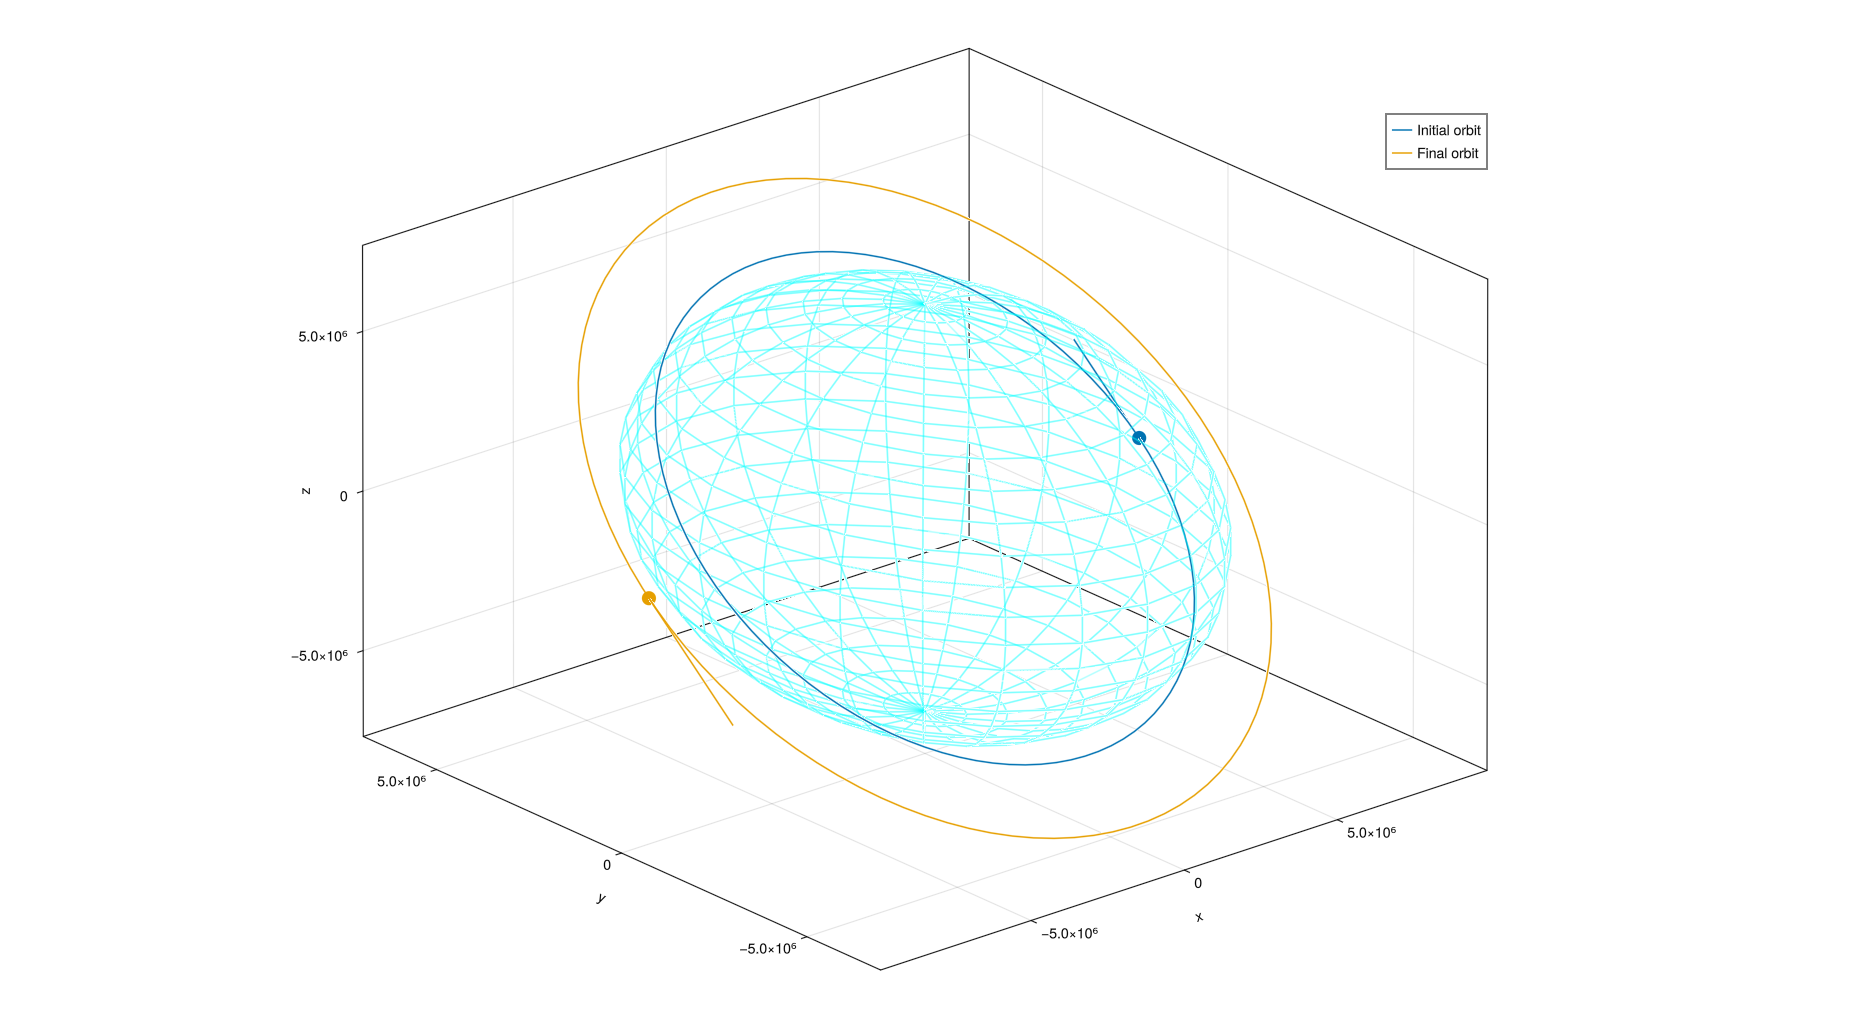
\includegraphics{../results/two_body/hohmann/scenario.png}
    \caption{Circle to Circle transfer scenario.}
    \label{fig:hohmann_scenario}
\end{figure}

\subsection{Noncoplanar rendez-vous}

A second, more challenging scenario is taken from \citeonline{interactive_primer_vector}, where a noncoplanar rendez-vous scenario is proposed and solved under the two body model. Again, the goal is validating the code against a published result under the two body model, and exploring how the optimal trajectory may be different under other more realistic models. The orbital parameters are given in Table~\ref{tab:noncop_rdv_orb_elems}, and multiple views of the scenario are shown in Figure~\ref{fig:noncop_rdv_scenario}. The transfer time is equal to two orbital periods of the target orbit.

% NCOP SCENARIO
\begin{table}[htbp]
    \centering
    \begin{tabular}{ccc} \toprule
        Element & Initial & Final \\ \midrule
        \(a\)      & \(6748.1\) km         & \(6778.1\) km   \\
        \(e\)      & \(0.0\)            & \(0.0\)        \\
        \(i\)      & \(42.1^\circ\)      & \(42.0^\circ\) \\
        \(\Omega\) & \(120.2^\circ\)   & \(120.0^\circ\)  \\
        \(\omega\) & \(0.0^\circ\)  & \(0.0^\circ\)  \\
        \(\theta\) & \(175.0^\circ\)  & \(180.0^\circ\)  \\ 
        Transfer time & \multicolumn{2}{c}{\(11107.158\)} \\\bottomrule
    \end{tabular}
    \caption{Orbital elements used for the noncoplanar rendez-vous case analysis}
    \label{tab:noncop_rdv_orb_elems}
\end{table}
% NCOP SCENARIO


\begin{figure}[htbp]
    \centering
    \begin{subfigure}{0.49\linewidth}
        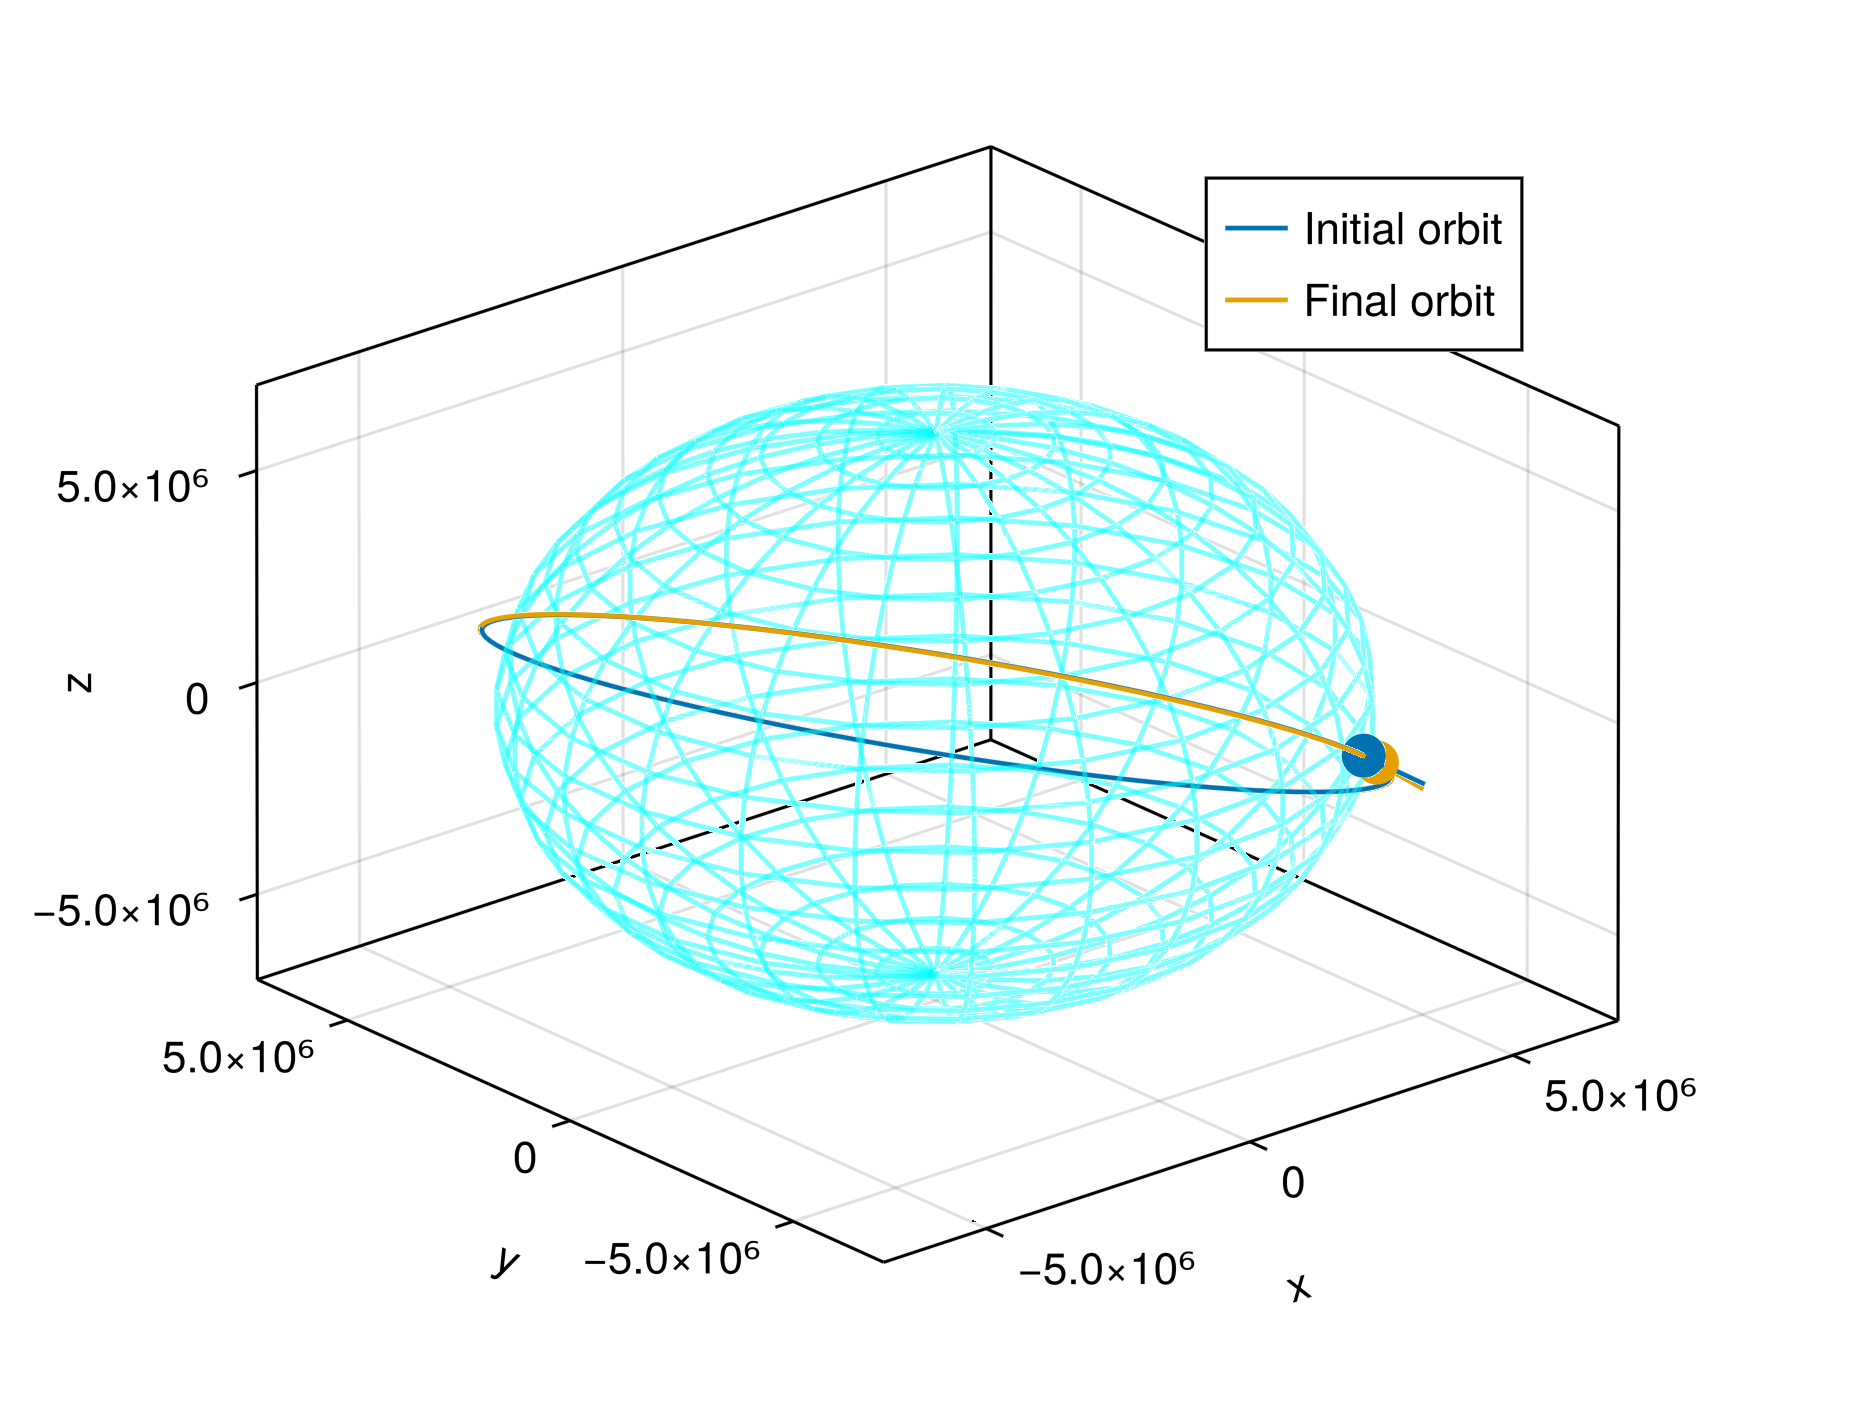
\includegraphics[width=\linewidth]{../results/two_body/ipv_noncop/scenario_3d.png}
        \caption{3D view.}
    \end{subfigure}
    \begin{subfigure}{0.49\linewidth}
        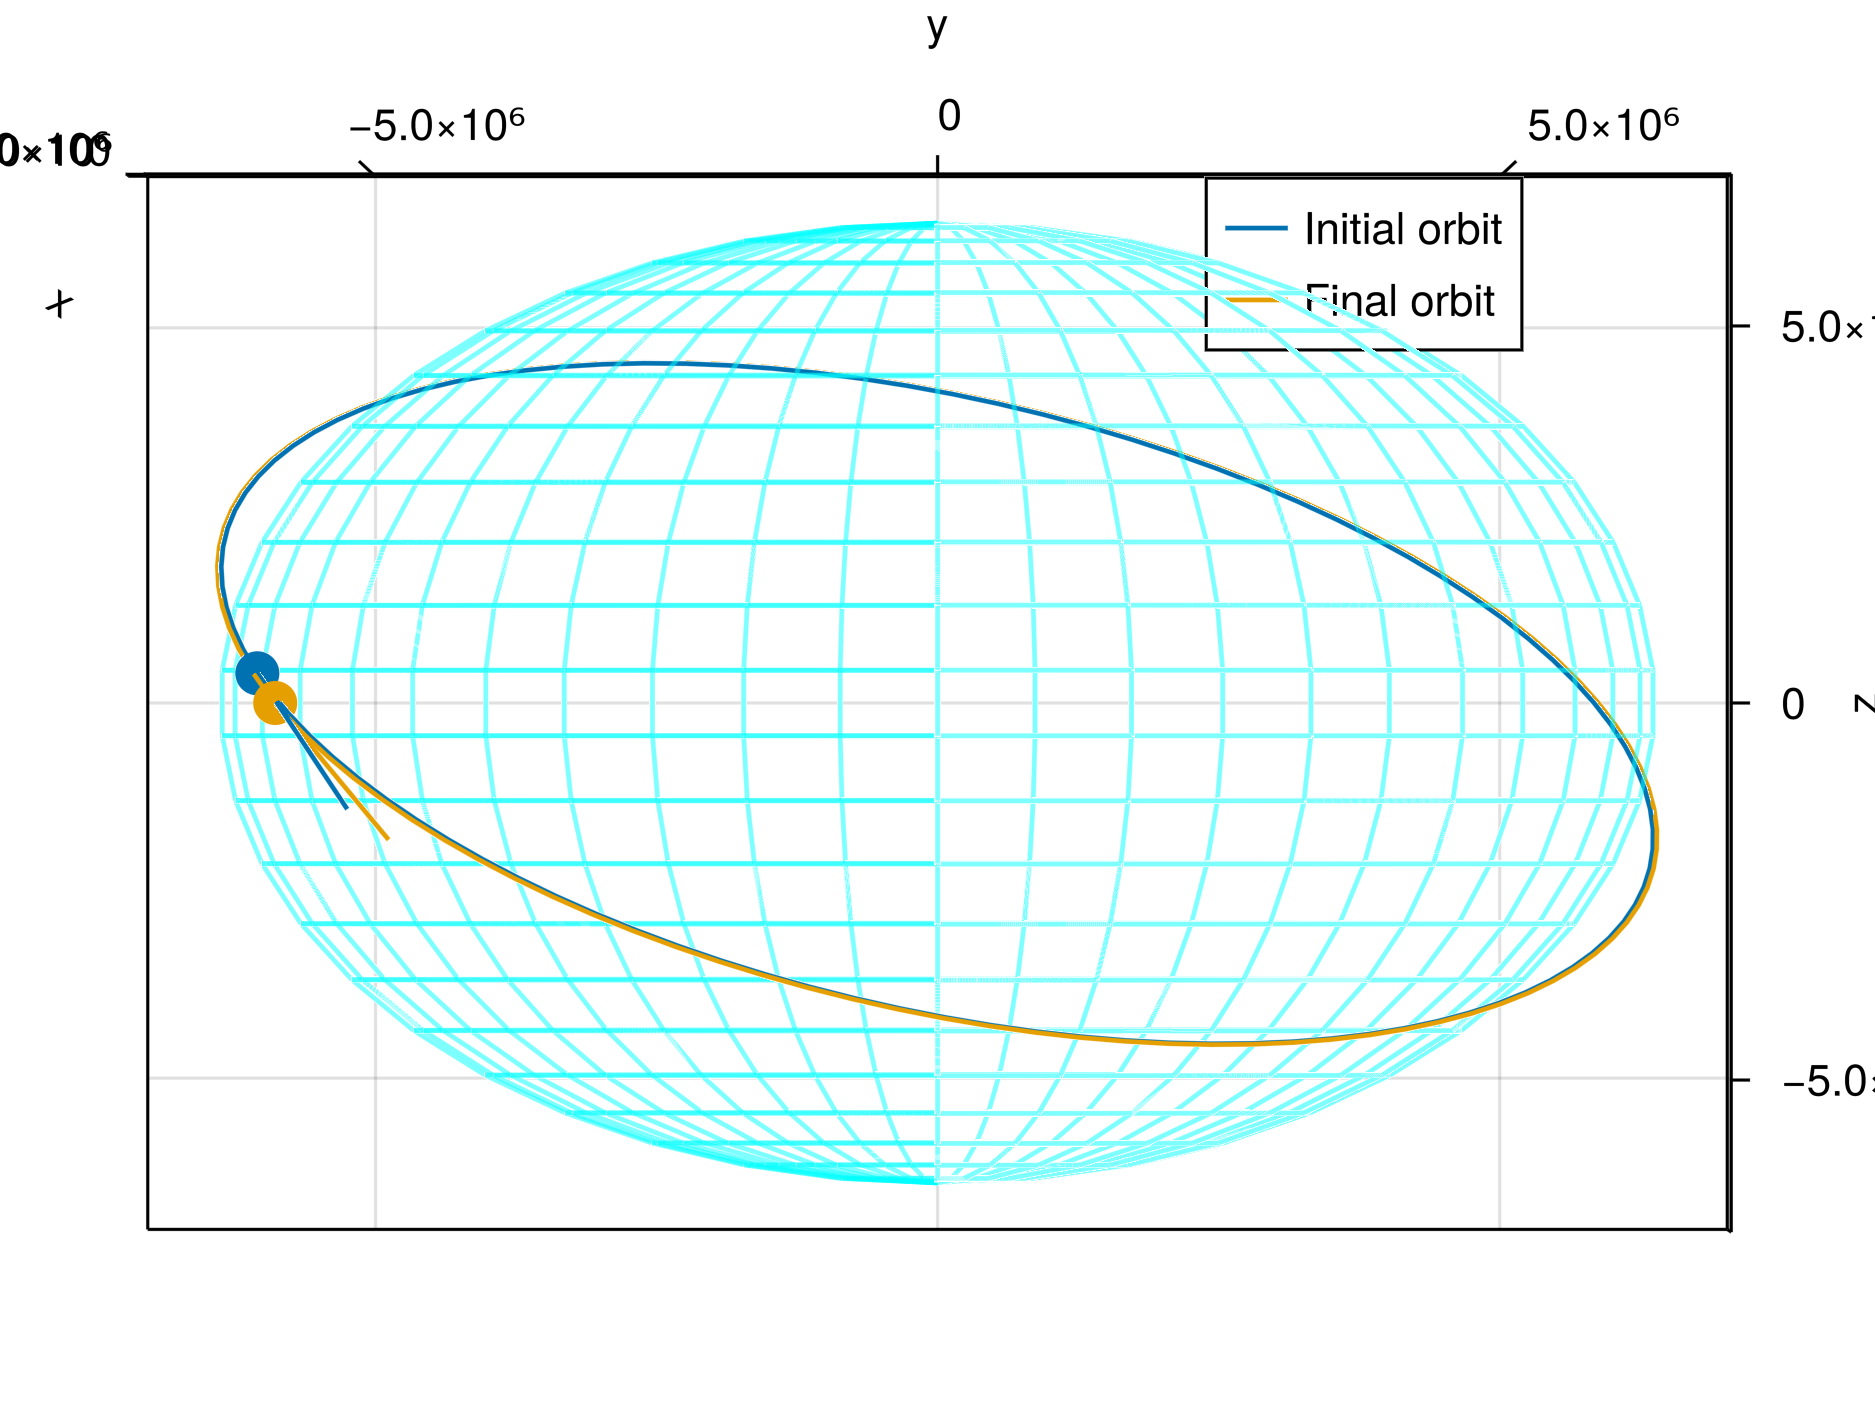
\includegraphics[width=\linewidth]{../results/two_body/ipv_noncop/scenario_x+.png}
        \caption{View from x+ axis.}
    \end{subfigure}
    \begin{subfigure}{0.49\linewidth}
        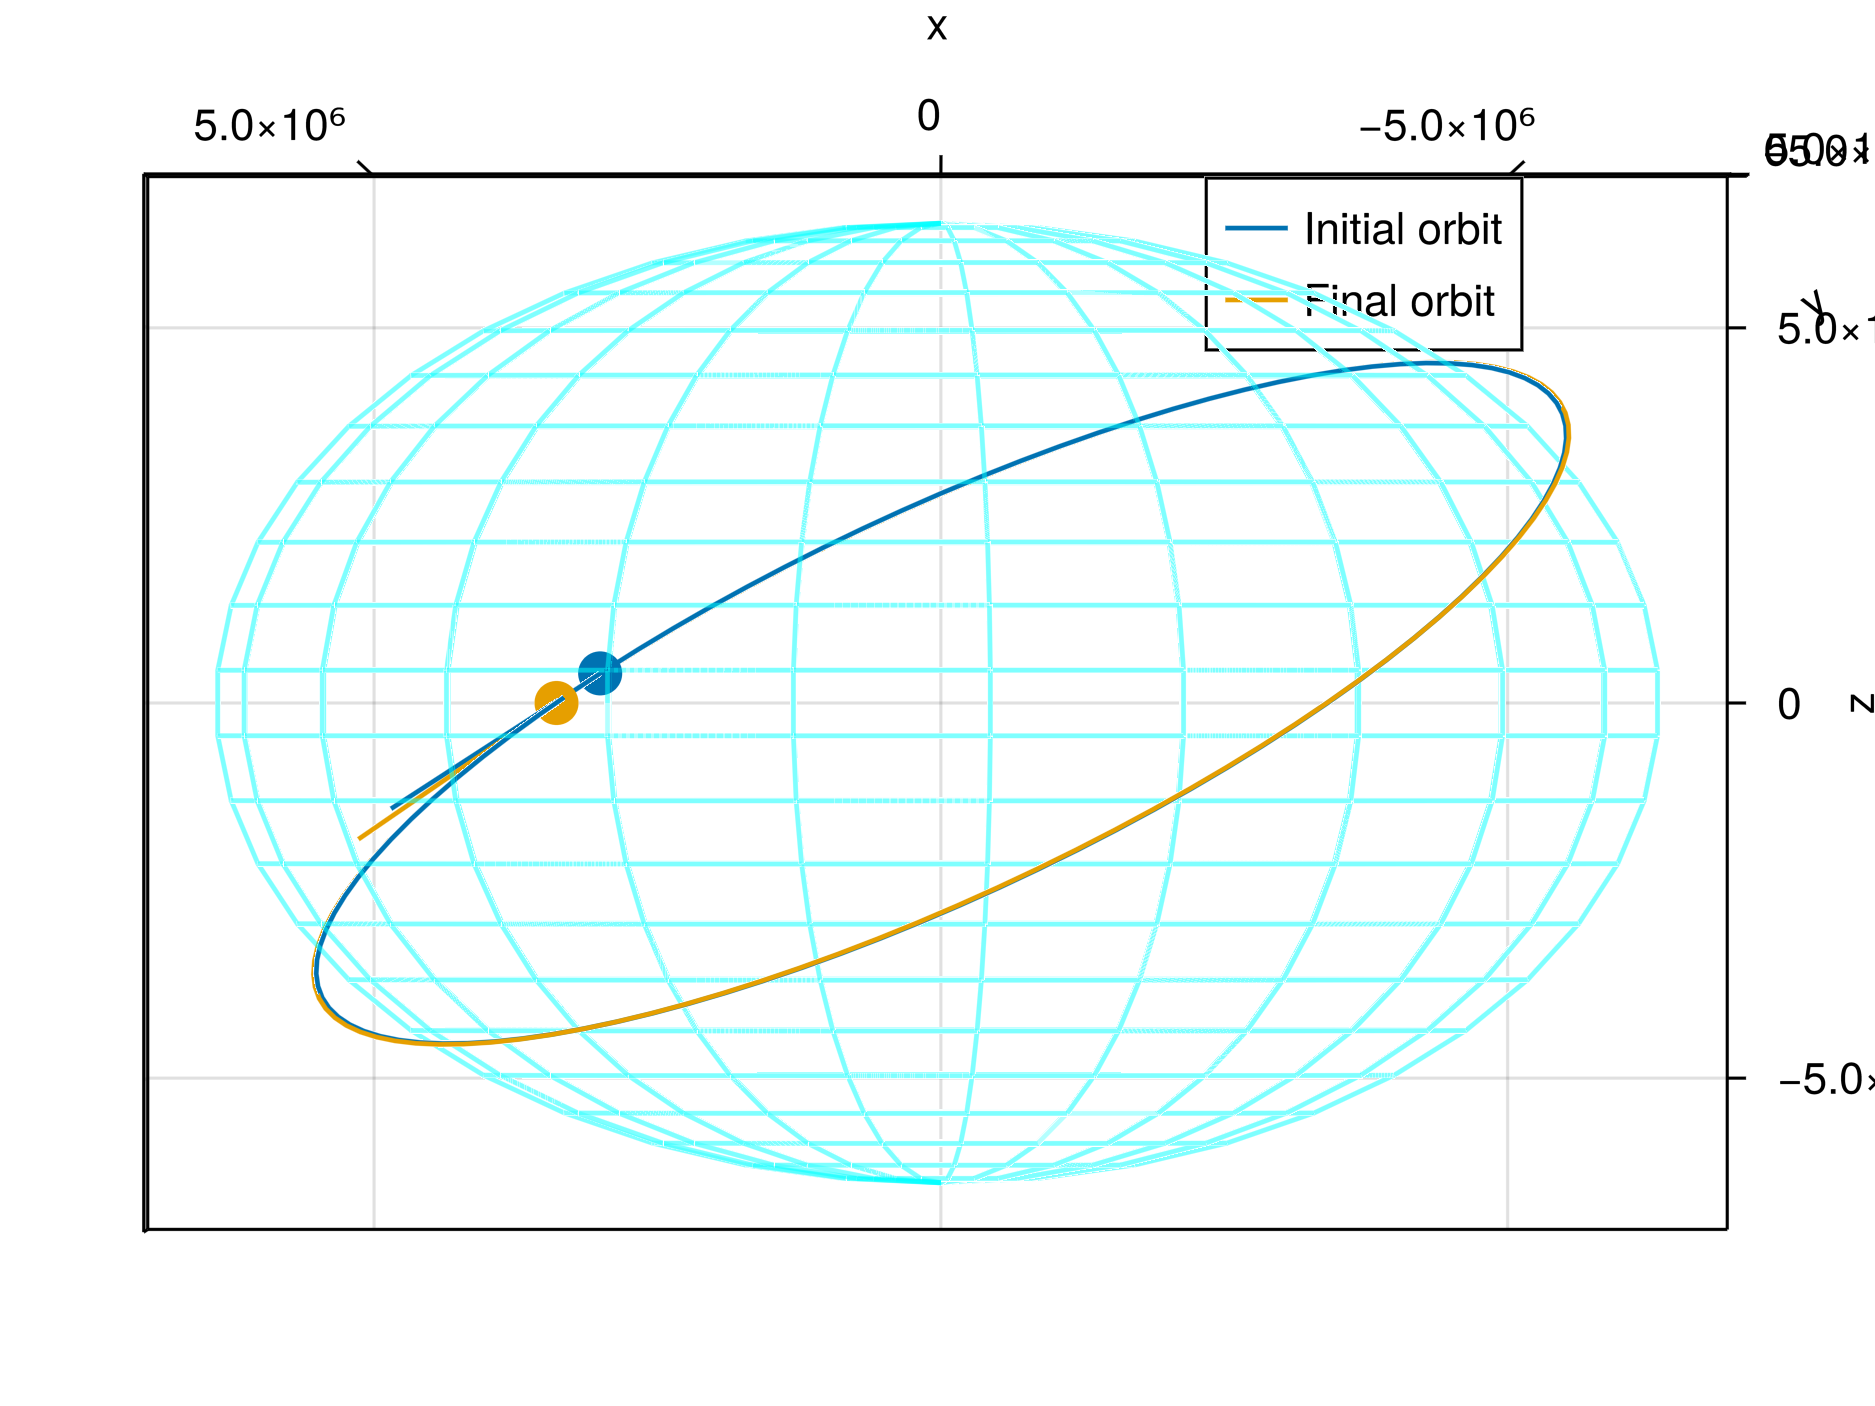
\includegraphics[width=\linewidth]{../results/two_body/ipv_noncop/scenario_y+.png}
        \caption{View from y+ axis.}
    \end{subfigure}
    \begin{subfigure}{0.49\linewidth}
        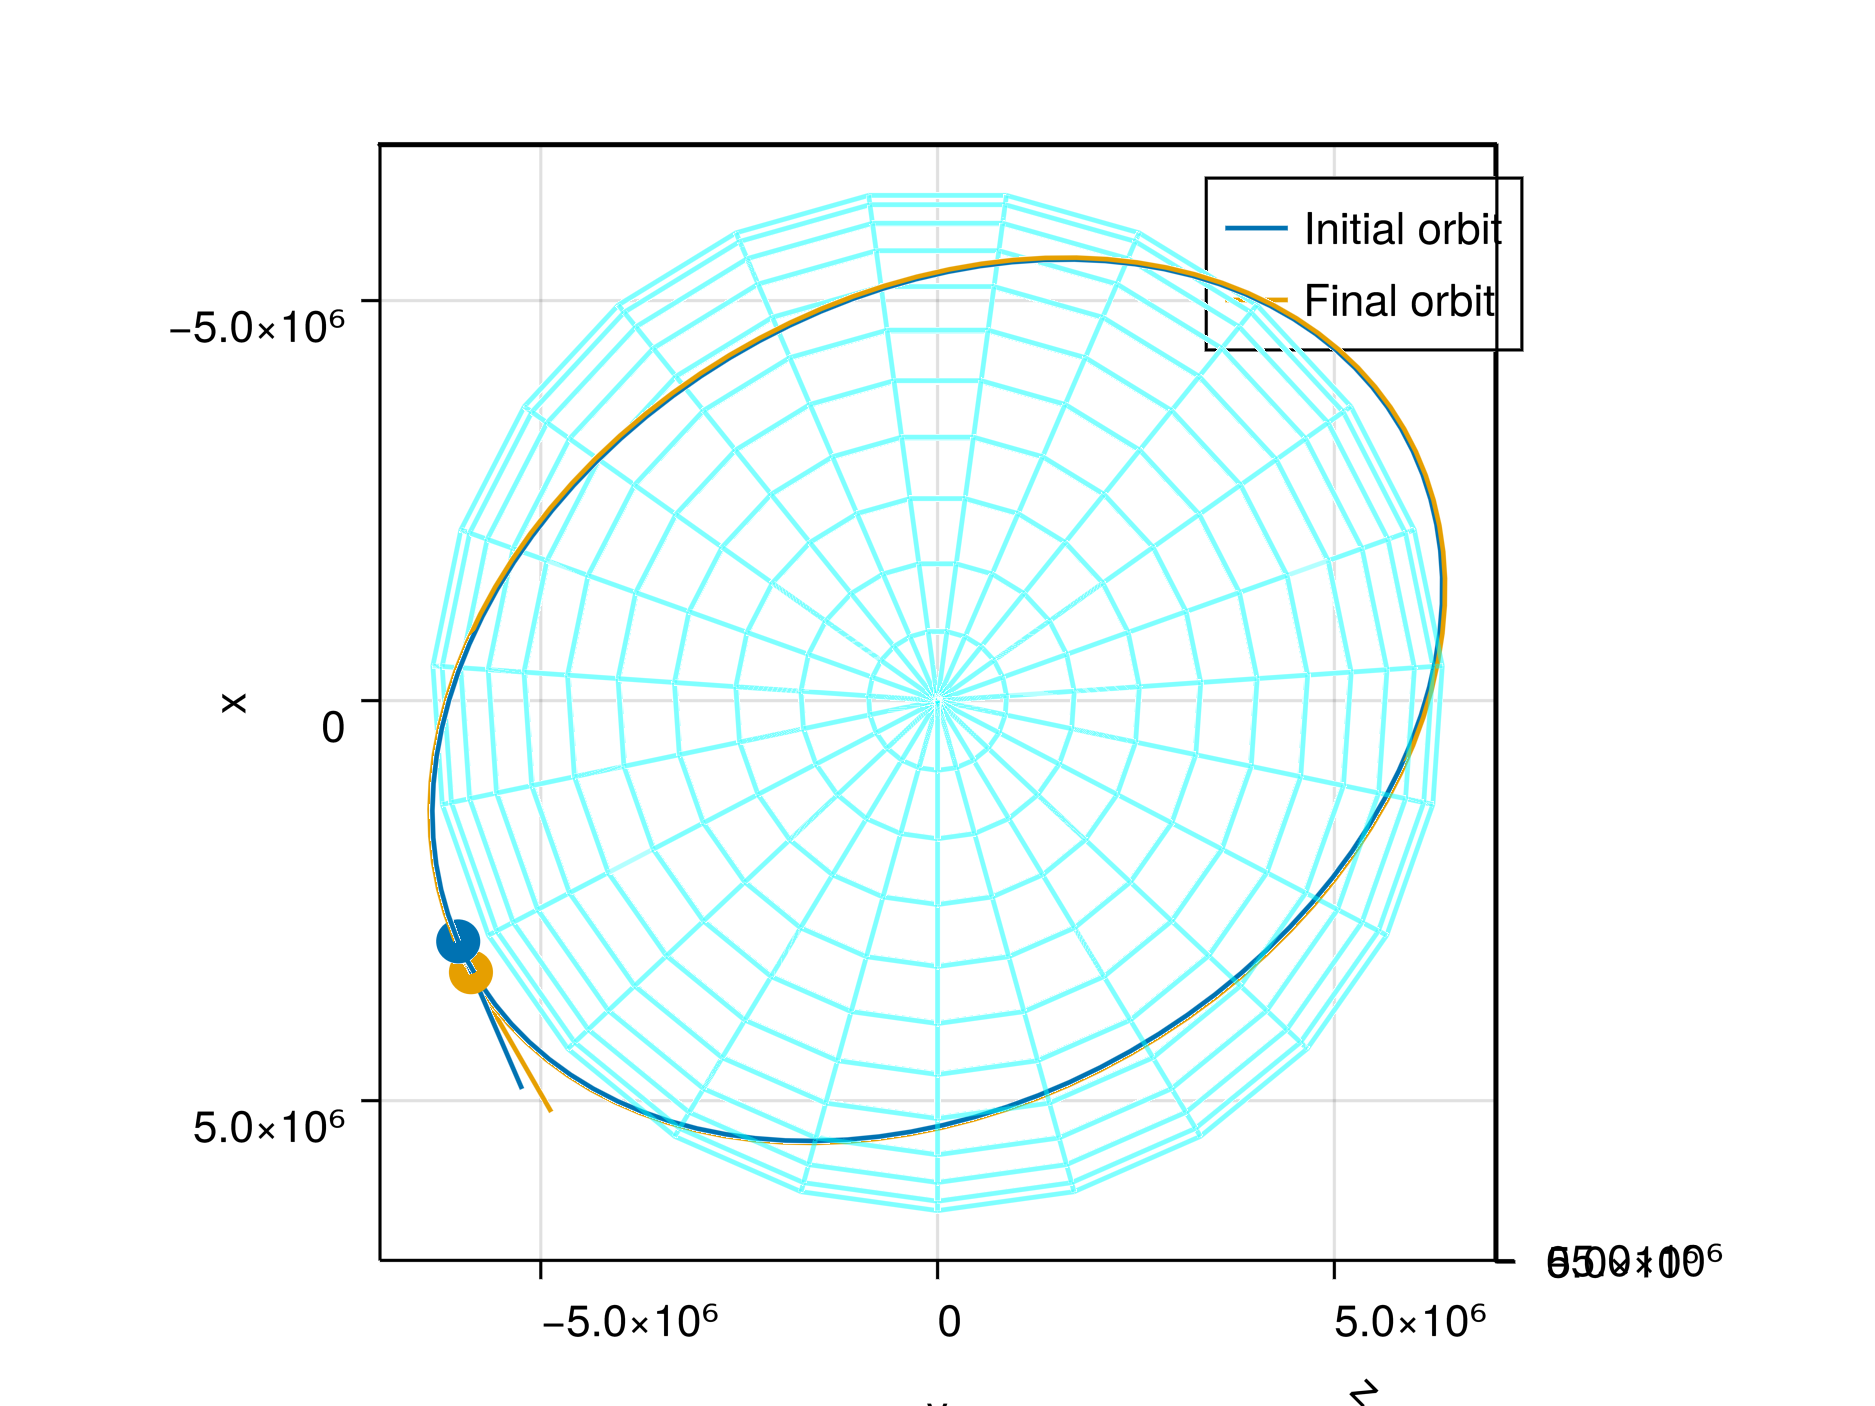
\includegraphics[width=\linewidth]{../results/two_body/ipv_noncop/scenario_z+.png}
        \caption{View from z+ axis.}
    \end{subfigure}
    \caption{Noncoplanar rendez-vous scenario 3D view and projections}
    \label{fig:noncop_rdv_scenario}
\end{figure}

\FloatBarrier
\section{Two Body}

The results for all scenarios under the two body model are presented in the following. All primer vector histories in this section were calculated with the Glandorf, STM and ODE methods, to numerically show they are equivalent. In all primer vector plots, vertical dashed lines indicate impulse times.

\subsection{Circle to Circle}

The circle to circle transfer scenario was first optimized for an \texttt{ICI} maneuver sequence. The results can be seen in Table~\ref{tab:tb_c2c_ICI_tab}, the primer vector trajectory can be seen in Figure~\ref{fig:tb_c2c_ICI_pv}, and the views of the optimized trajectory, in Figure~\ref{fig:tb_c2c_ICI_figs}. It can be seen that impulses at the starting and ending condition are capable of satisfying the necessary optimality conditions, and the analytical Hohmann of \(\Delta v_H = 887.56199 m/s\), computed from Equation~\eqref{eq:hohmann_deltav}, has been attained.

TODO try CICIC???

% TB C2C ICI
\begin{table}[htpb]
    \centering
    \begin{tabular}{cccc} \toprule
    \multicolumn{2}{c}{\textbf{Maneuver type}} & \multicolumn{2}{c}{\texttt{ICI}} \\ \midrule
    \(L\) (m) & \(T\) (s) & \(\varepsilon\) & \(\lVert \Delta \pos_{f} \rVert\) (m)    \\ \midrule
    8.0e6          & 1.0          & 1.00e-05                & 2.11019e-08                        \\ \midrule
    \(\max \lVert p \rVert\) & 1.0     & \textbf{Diagnostic}   & Local optimum        \\ \midrule
    \textbf{Impulse} & \(t\) (s) & \(\Delta v\) (m/s) & \(1 - p \cdot \hat{u}\) \\ \midrule
    1                 & 0.0          & 457.74489             & 0.0                    \\
    2                 & 3560.54079          & 429.8171             & 0.0                    \\\midrule
    \textbf{Total}   & 3560.54079          & 887.56199             &                     \\ \bottomrule   
    \end{tabular}
    \caption{Summary of optimization for Keplerian circle to circle \texttt{ICI} rendez-vous.}
    \label{tab:tb_ctc_ICI_tab}
\end{table}
% TB C2C ICI

\begin{figure}[htbp]
    \centering
    \begin{subfigure}{0.49\linewidth}
        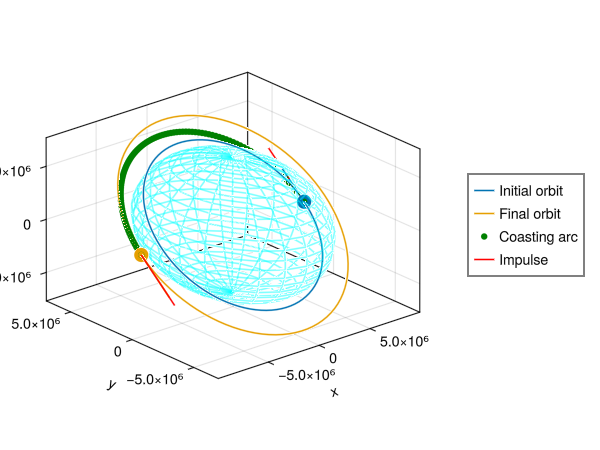
\includegraphics[width=\linewidth]{../results/two_body/hohmann/ICI_3d.png}
        \caption{3D view.}
    \end{subfigure}
    \begin{subfigure}{0.49\linewidth}
        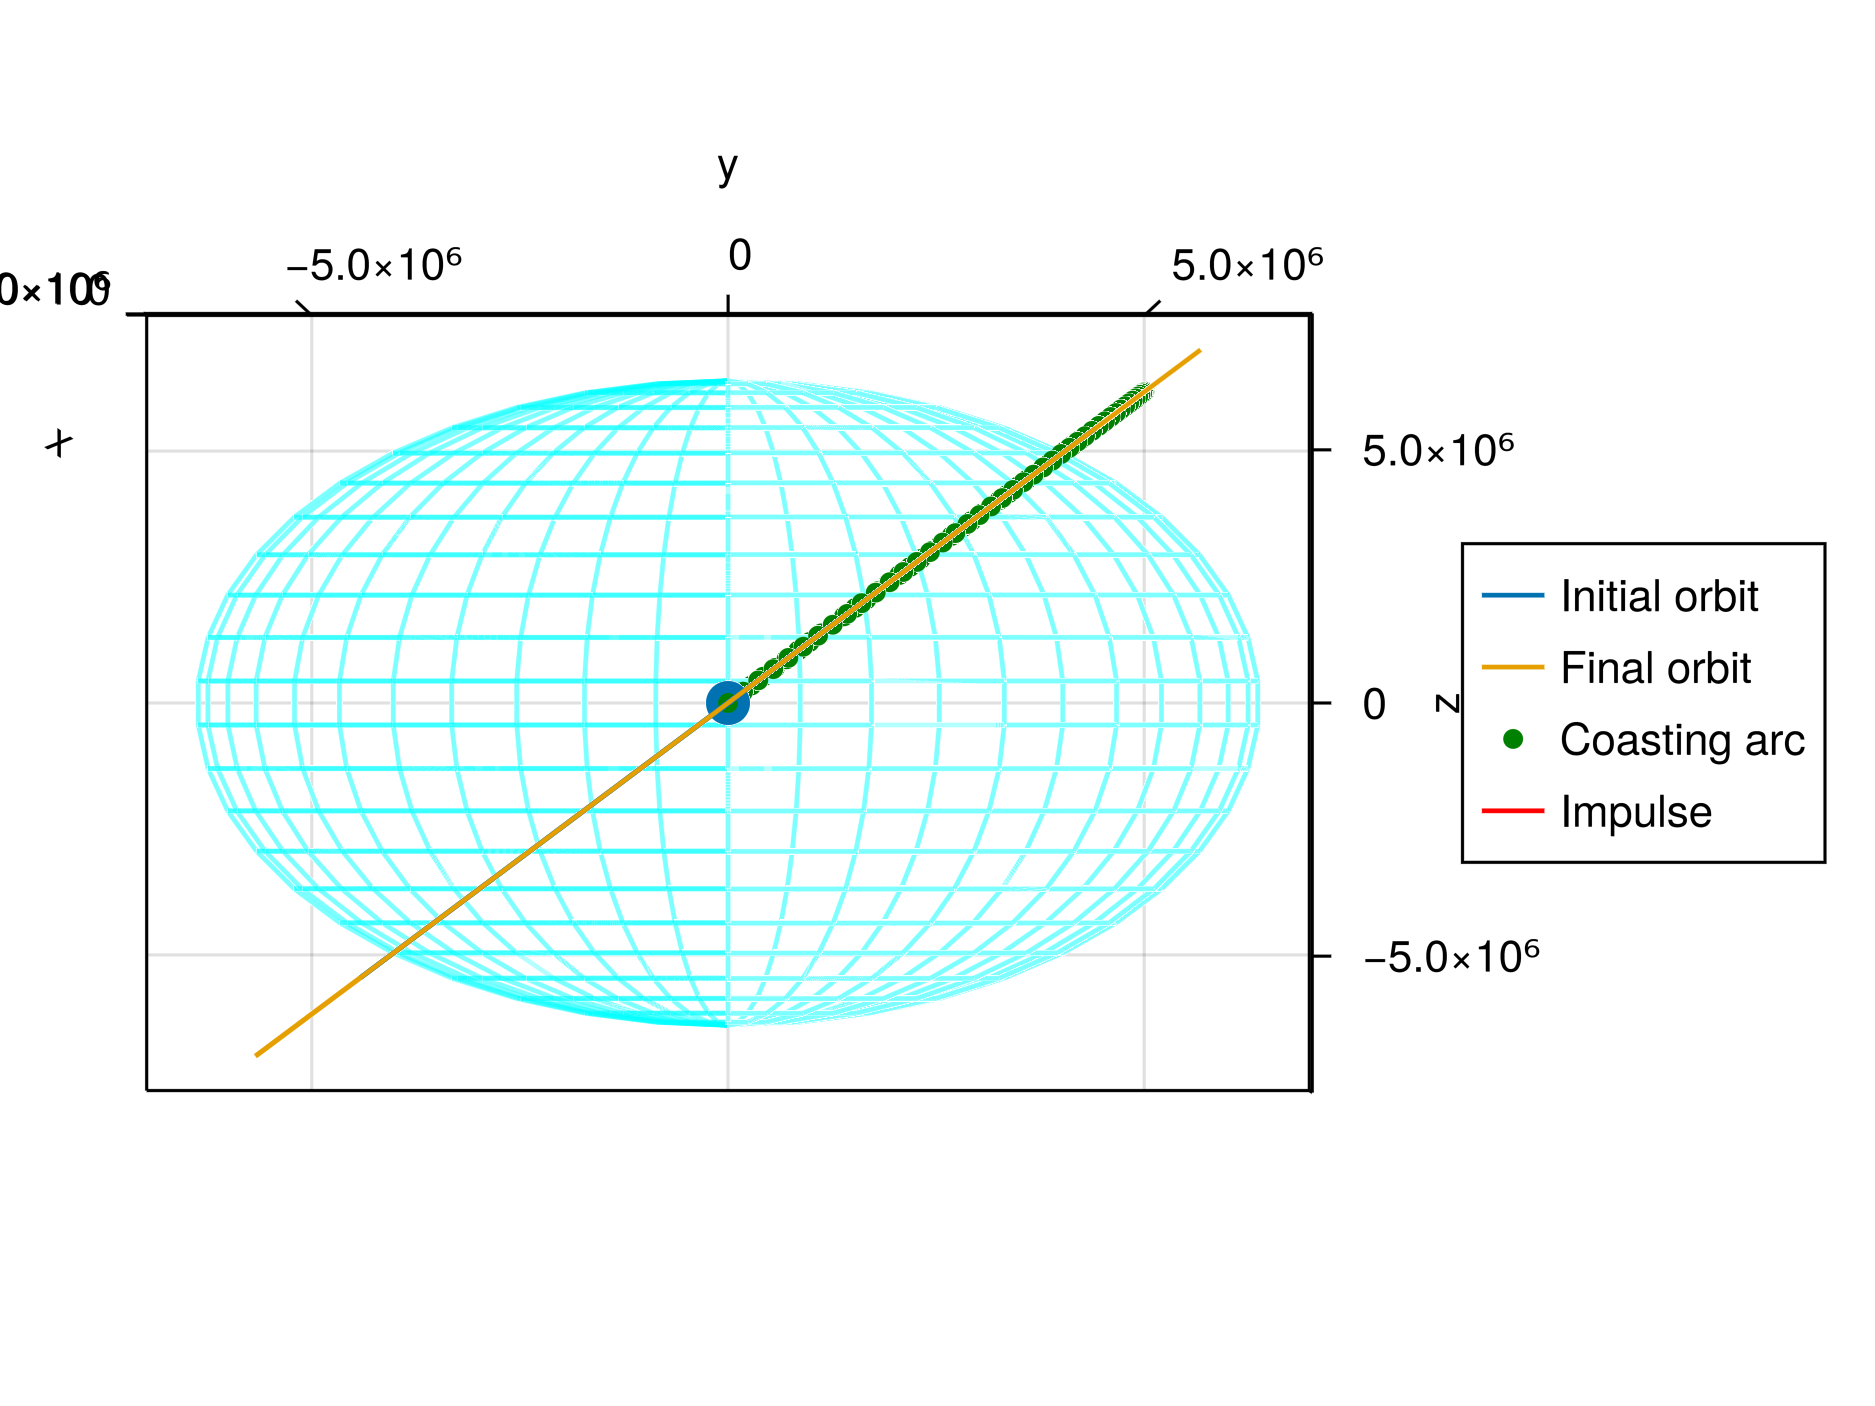
\includegraphics[width=\linewidth]{../results/two_body/hohmann/ICI_x+.png}
        \caption{View from x+ axis.}
    \end{subfigure}
    \begin{subfigure}{0.49\linewidth}
        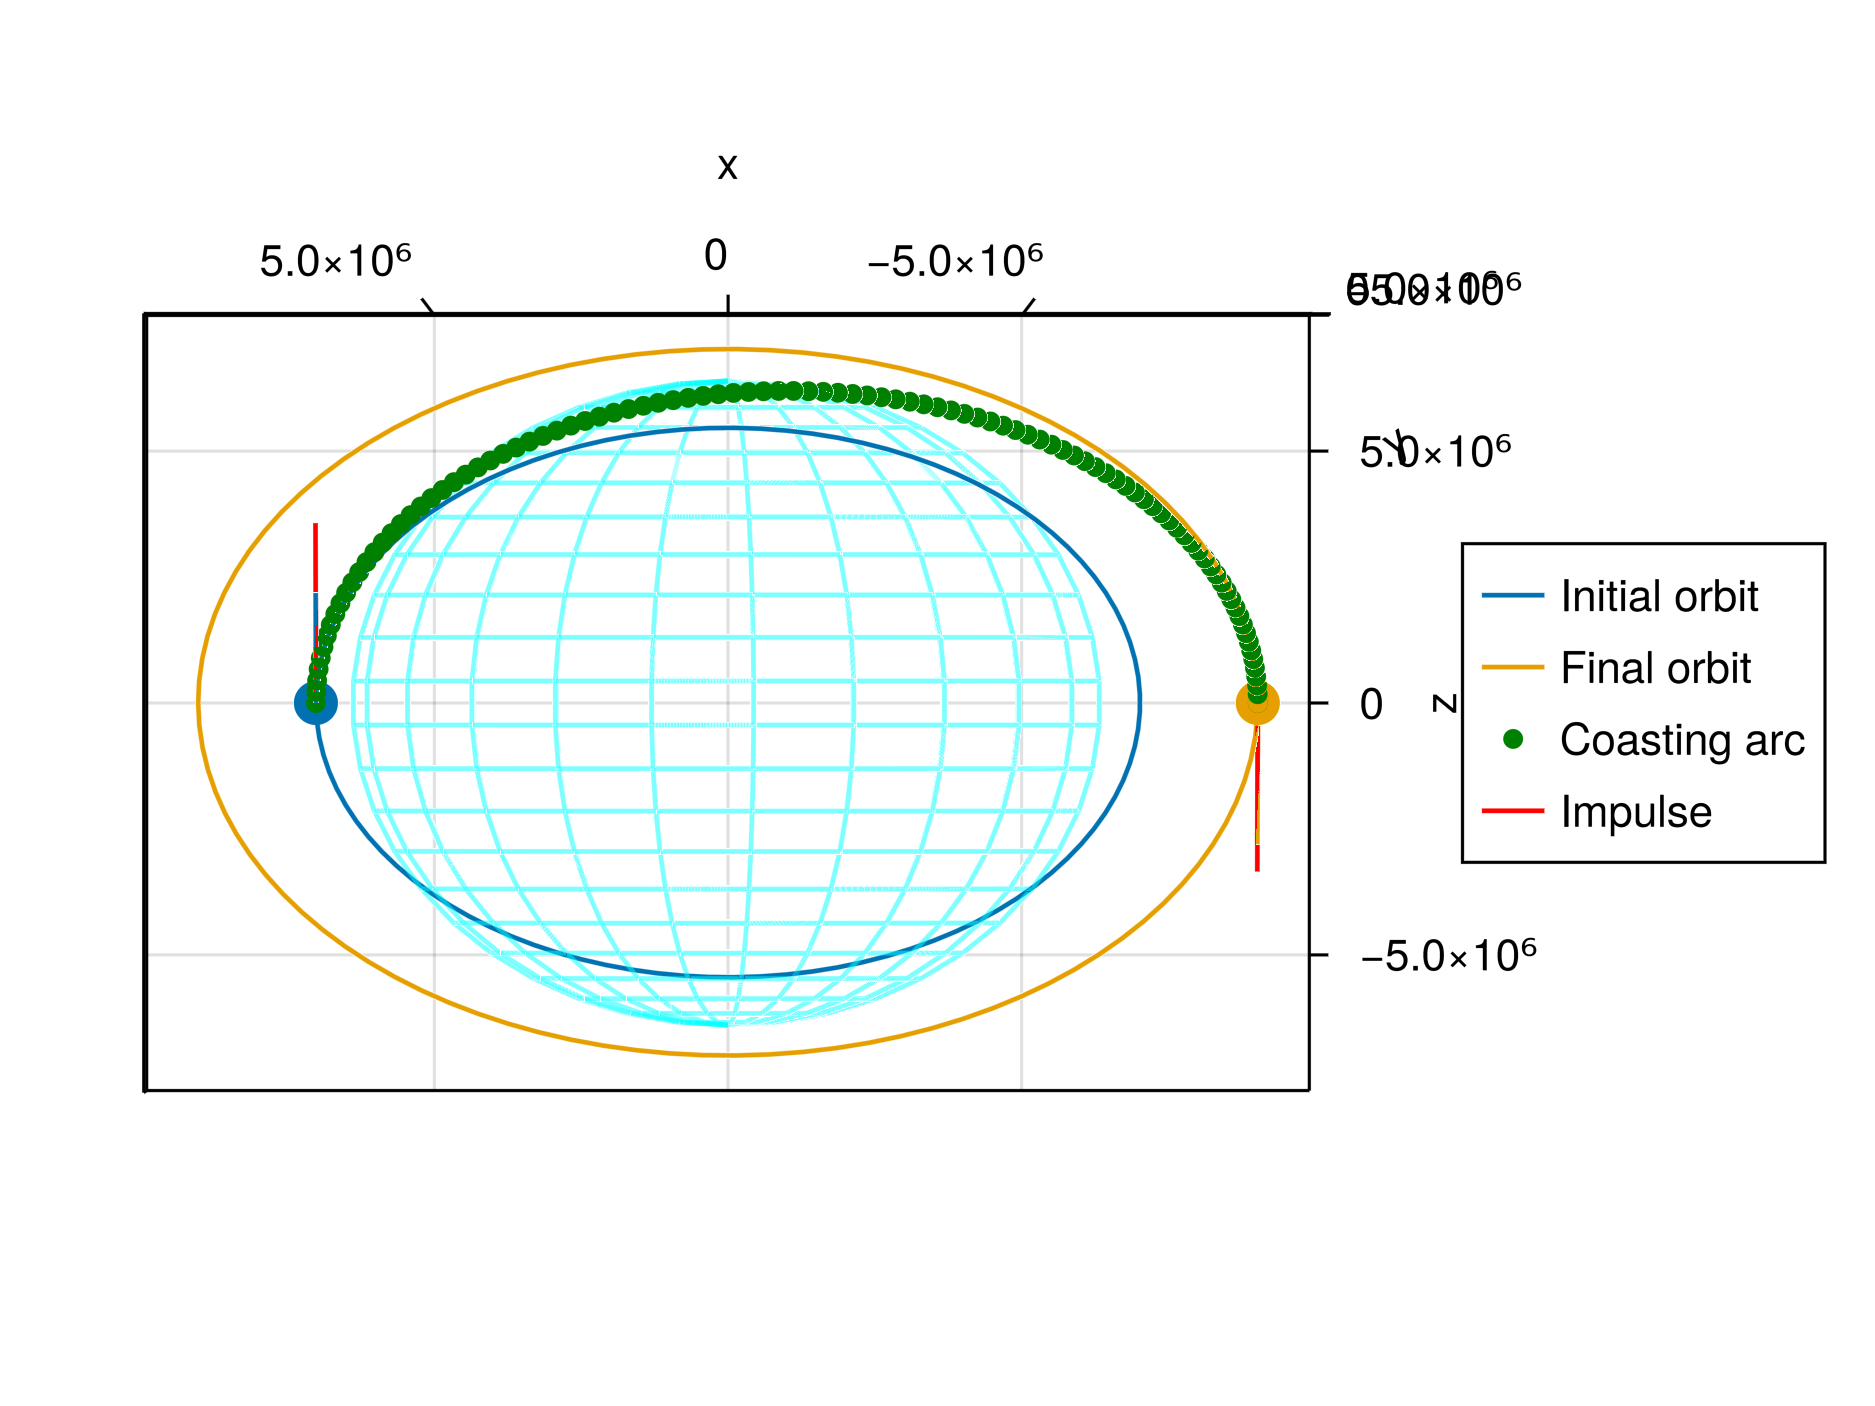
\includegraphics[width=\linewidth]{../results/two_body/hohmann/ICI_y+.png}
        \caption{View from y+ axis.}
    \end{subfigure}
    \begin{subfigure}{0.49\linewidth}
        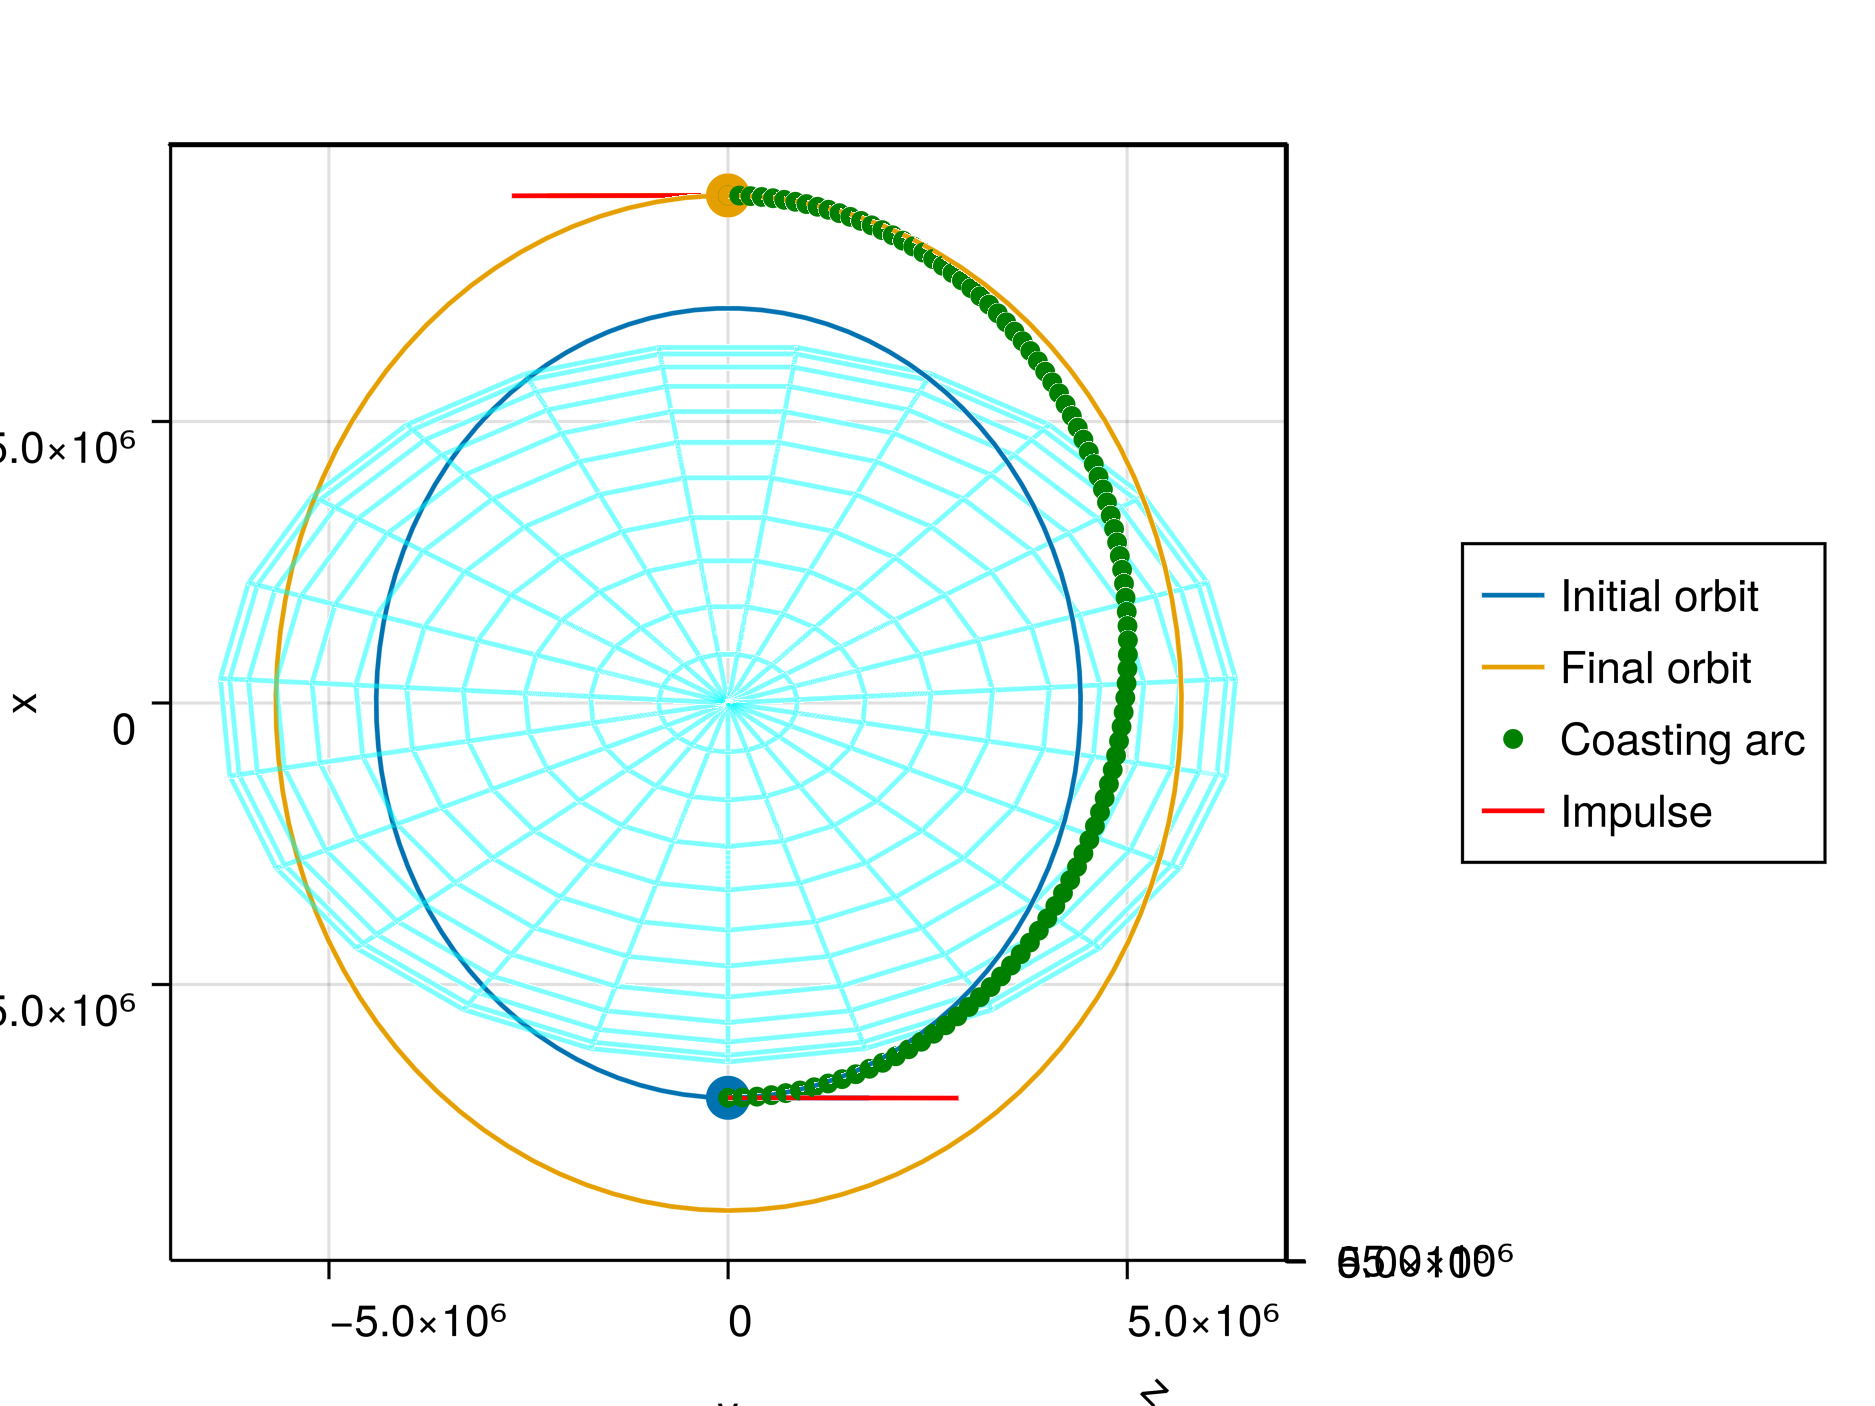
\includegraphics[width=\linewidth]{../results/two_body/hohmann/ICI_z+.png}
        \caption{View from z+ axis.}
    \end{subfigure}
    \caption{Circle to circle \texttt{ICI} maneuver 3D view and projections}
    \label{fig:tb_c2c_ICI_figs}
\end{figure}

\begin{figure}[htbp]
    \centering
    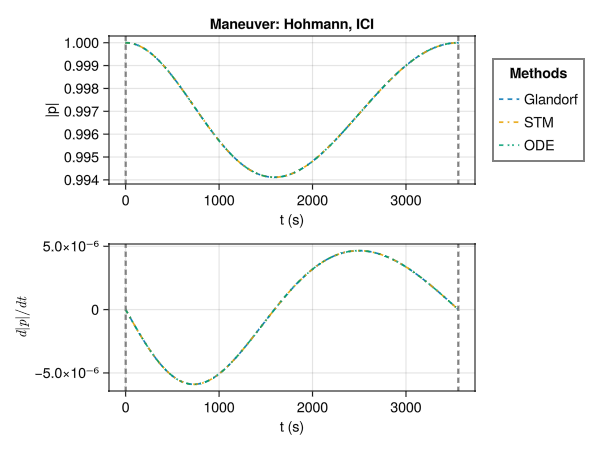
\includegraphics[width=\linewidth]{../results/two_body/hohmann/ICI_primer_vector.png}
    \caption{Primer vector trajectory for two body circle to circle \texttt{ICI} rendez-vous.}
    \label{fig:tb_c2c_ICI_pv}
\end{figure}

\subsection{Noncoplanar rendez-vous}

The more complex noncoplanar rendez-vous case was optimized with an \texttt{ICI} maneuver at first. The maneuver's summary, primer vector trajectory, and spatial views can be seen in Table~\ref{tab:tb_ncop_ICI_tab}, Figure~\ref{fig:tb_ncop_ICI_pv} and Figure~\ref{fig:tb_ncop_ICI_figs}. The primer vector history shows that this is a local optimum, but physical intuition suggests that there are less aggressive maneuvers that can solve the maneuver problem. In order to find better optima, the problem must be relaxed: the introduction of initial and final coasts increases the degrees of freedom of the control, possibly allowing for a better cost.

% TB NCOP ICI
\begin{table}[htpb]
    \centering
    \begin{tabular}{cccc} \toprule
    \multicolumn{2}{c}{\textbf{Maneuver type}} & \multicolumn{2}{c}{ICI} \\ \midrule
    \(L\) (m) & \(T\) (s) & \(\varepsilon\) & \(\Delta x_{f}\) (m)    \\ \midrule
    6.7631e6          & 11107.158          & 1.00e-06                & 0.0                        \\ \midrule
    \(\max \lVert p \rVert\) & 1.0     & \textbf{Diagnostic}   & Local optimum        \\ \midrule
    \textbf{Impulse} & \(t\) (s) & \(\Delta v\) (m/s) & \(1 - p \cdot \hat{u}\) \\ \midrule
    1                 & 0.0          & 11740.94035             & -0.0                    \\
    2                 & 11107.1576          & 11708.69678             & -0.0                    \\\midrule
    \textbf{Total}   & 11107.1576          & 23449.63713             &                     \\ \bottomrule   
    \end{tabular}
    \caption{Summary of optimization for two body noncoplanar \texttt{ICI} rendez-vous.}
    \label{tab:tb_ncop_ICI_tab}
\end{table}
% TB NCOP ICI

\begin{figure}[htbp]
    \centering
    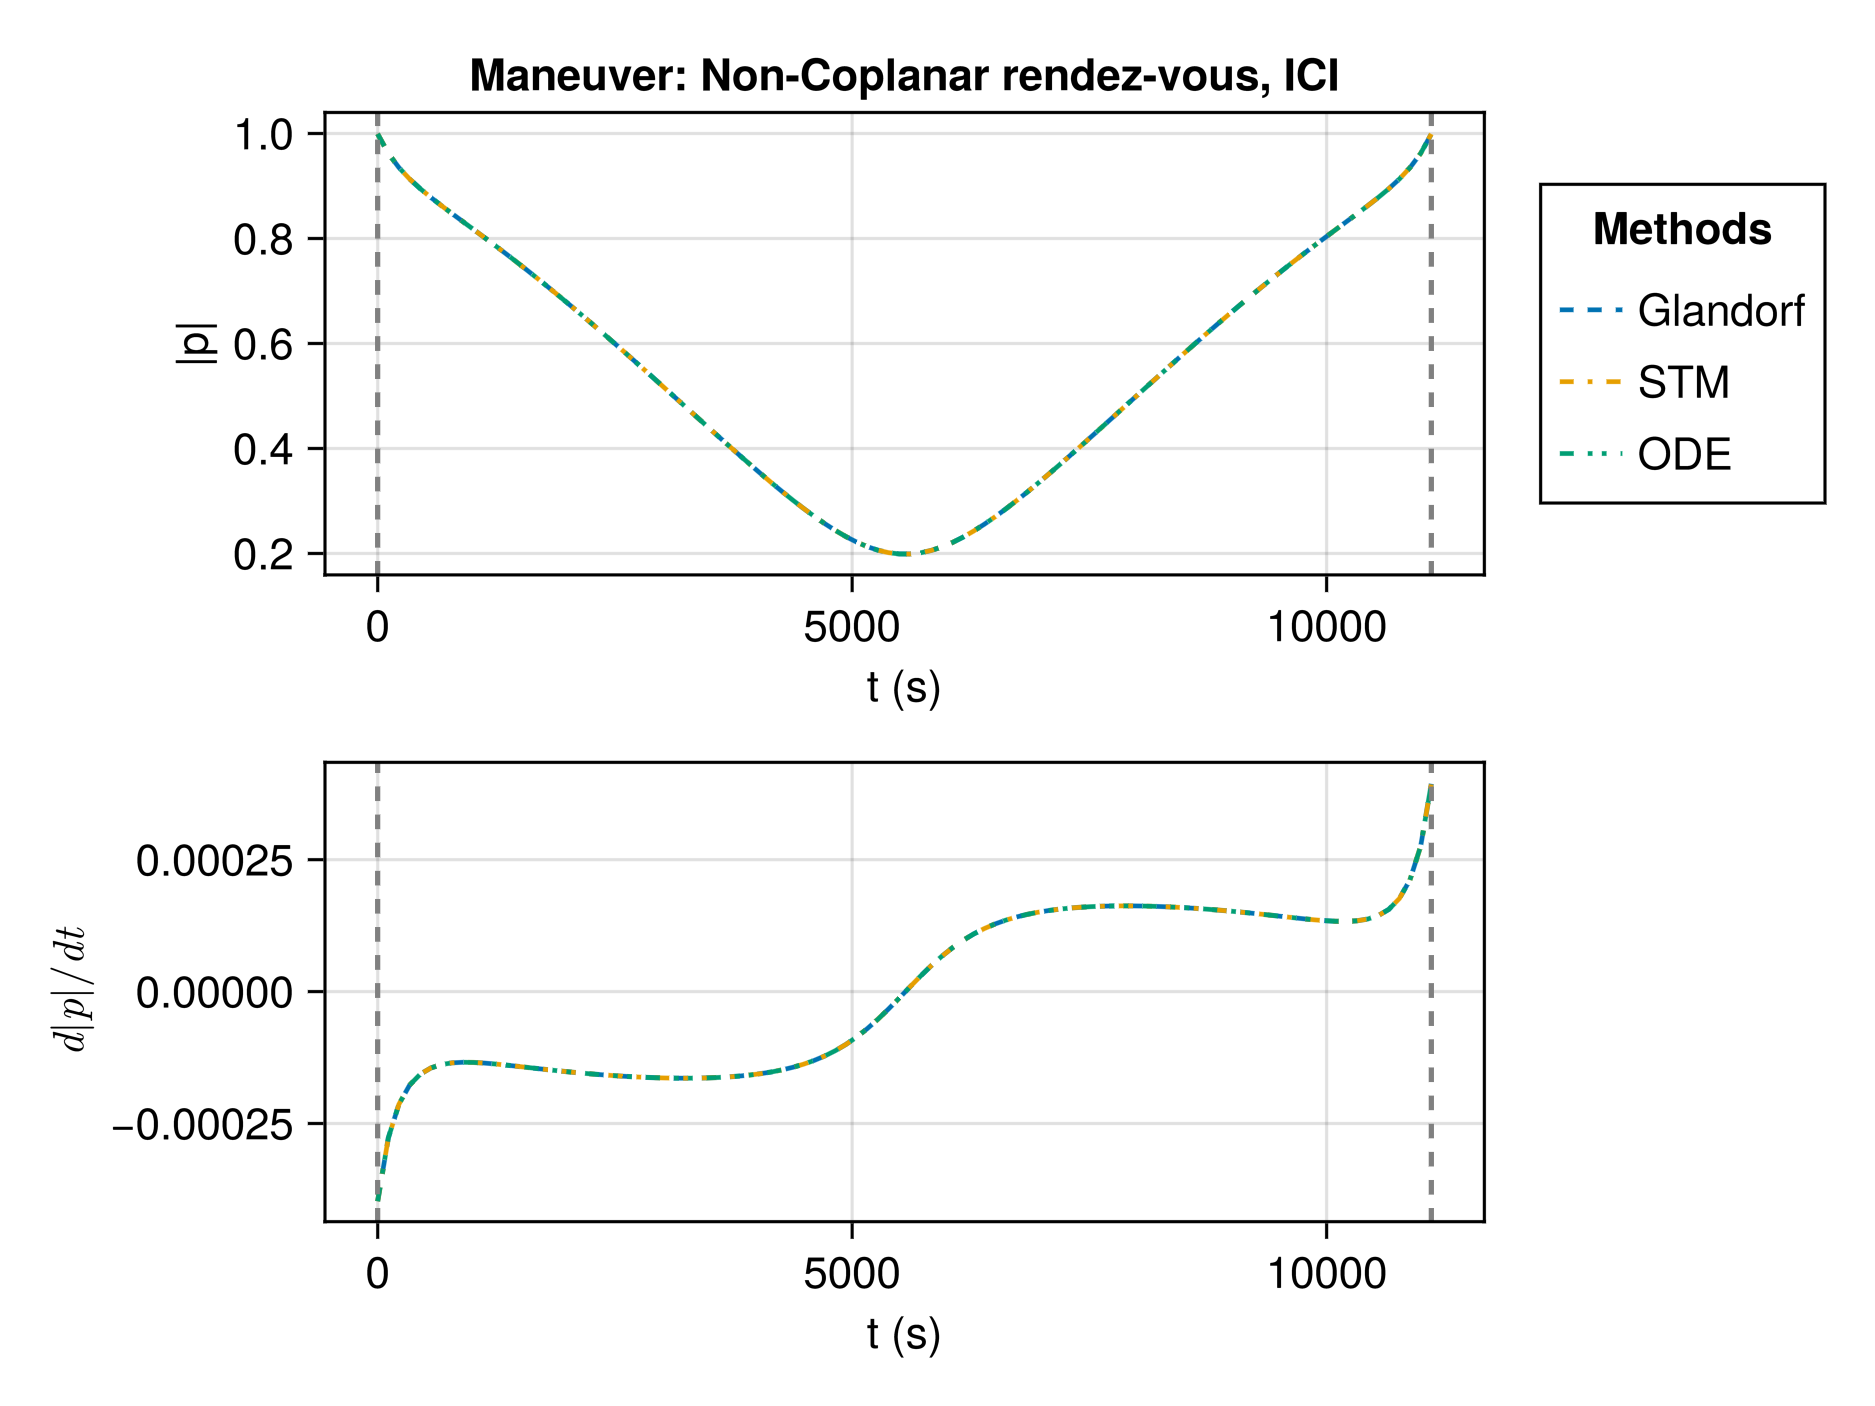
\includegraphics[width=\linewidth]{../results/two_body/ipv_noncop/ICI_primer_vector.png}
    \caption{Primer vector trajectory for two body noncoplanar \texttt{ICI} rendez-vous.}
    \label{fig:tb_ncop_ICI_pv}
\end{figure}

\begin{figure}[htbp]
    \centering
    \begin{subfigure}{0.49\linewidth}
        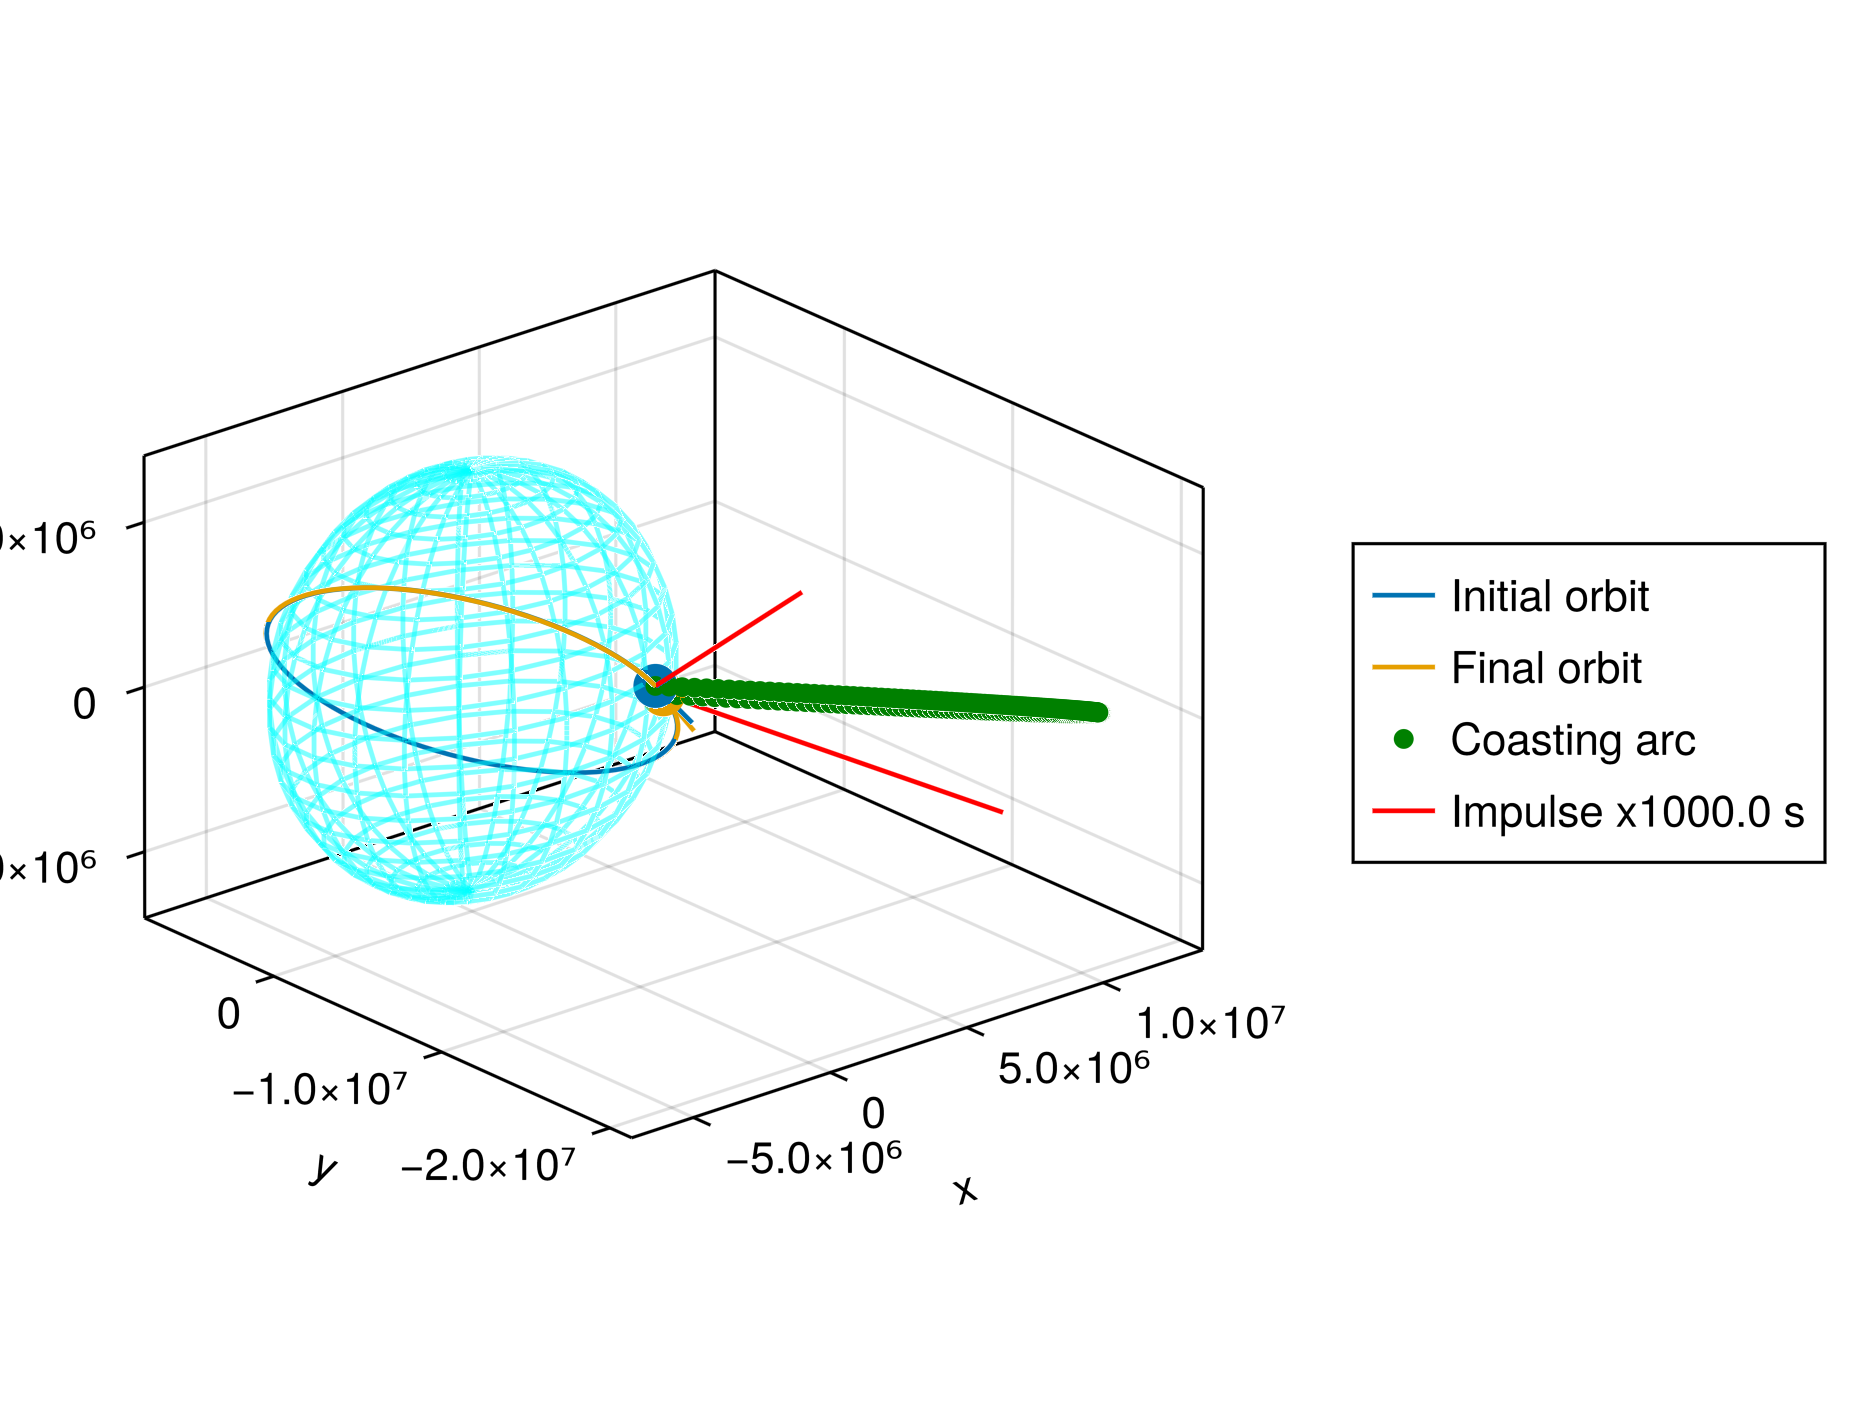
\includegraphics[width=\linewidth]{../results/two_body/ipv_noncop/ICI_3d.png}
        \caption{3D view.}
    \end{subfigure}
    \begin{subfigure}{0.49\linewidth}
        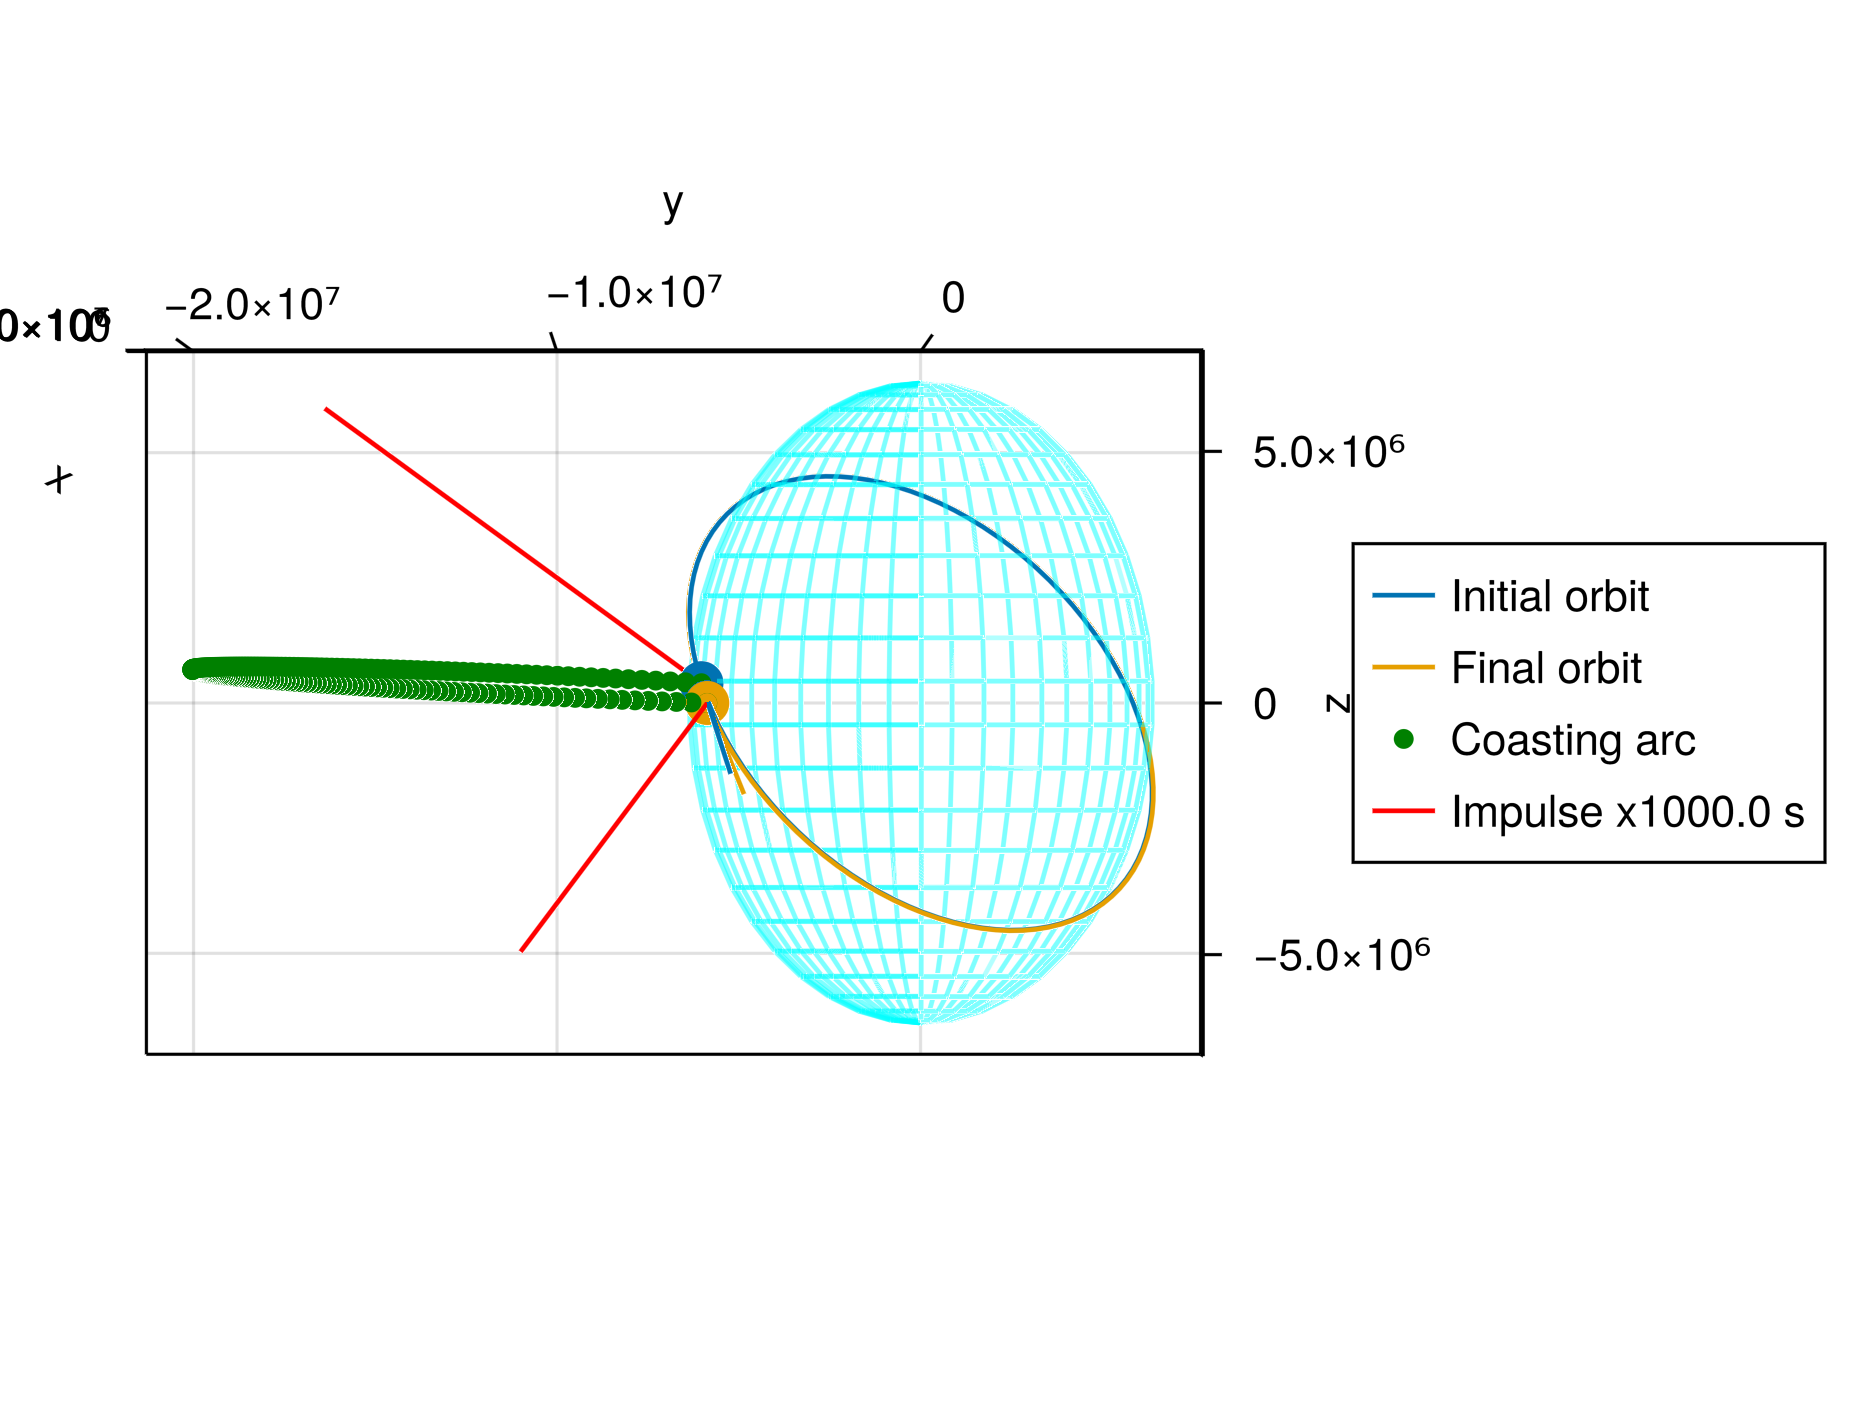
\includegraphics[width=\linewidth]{../results/two_body/ipv_noncop/ICI_x+.png}
        \caption{View from x+ axis.}
    \end{subfigure}
    \begin{subfigure}{0.49\linewidth}
        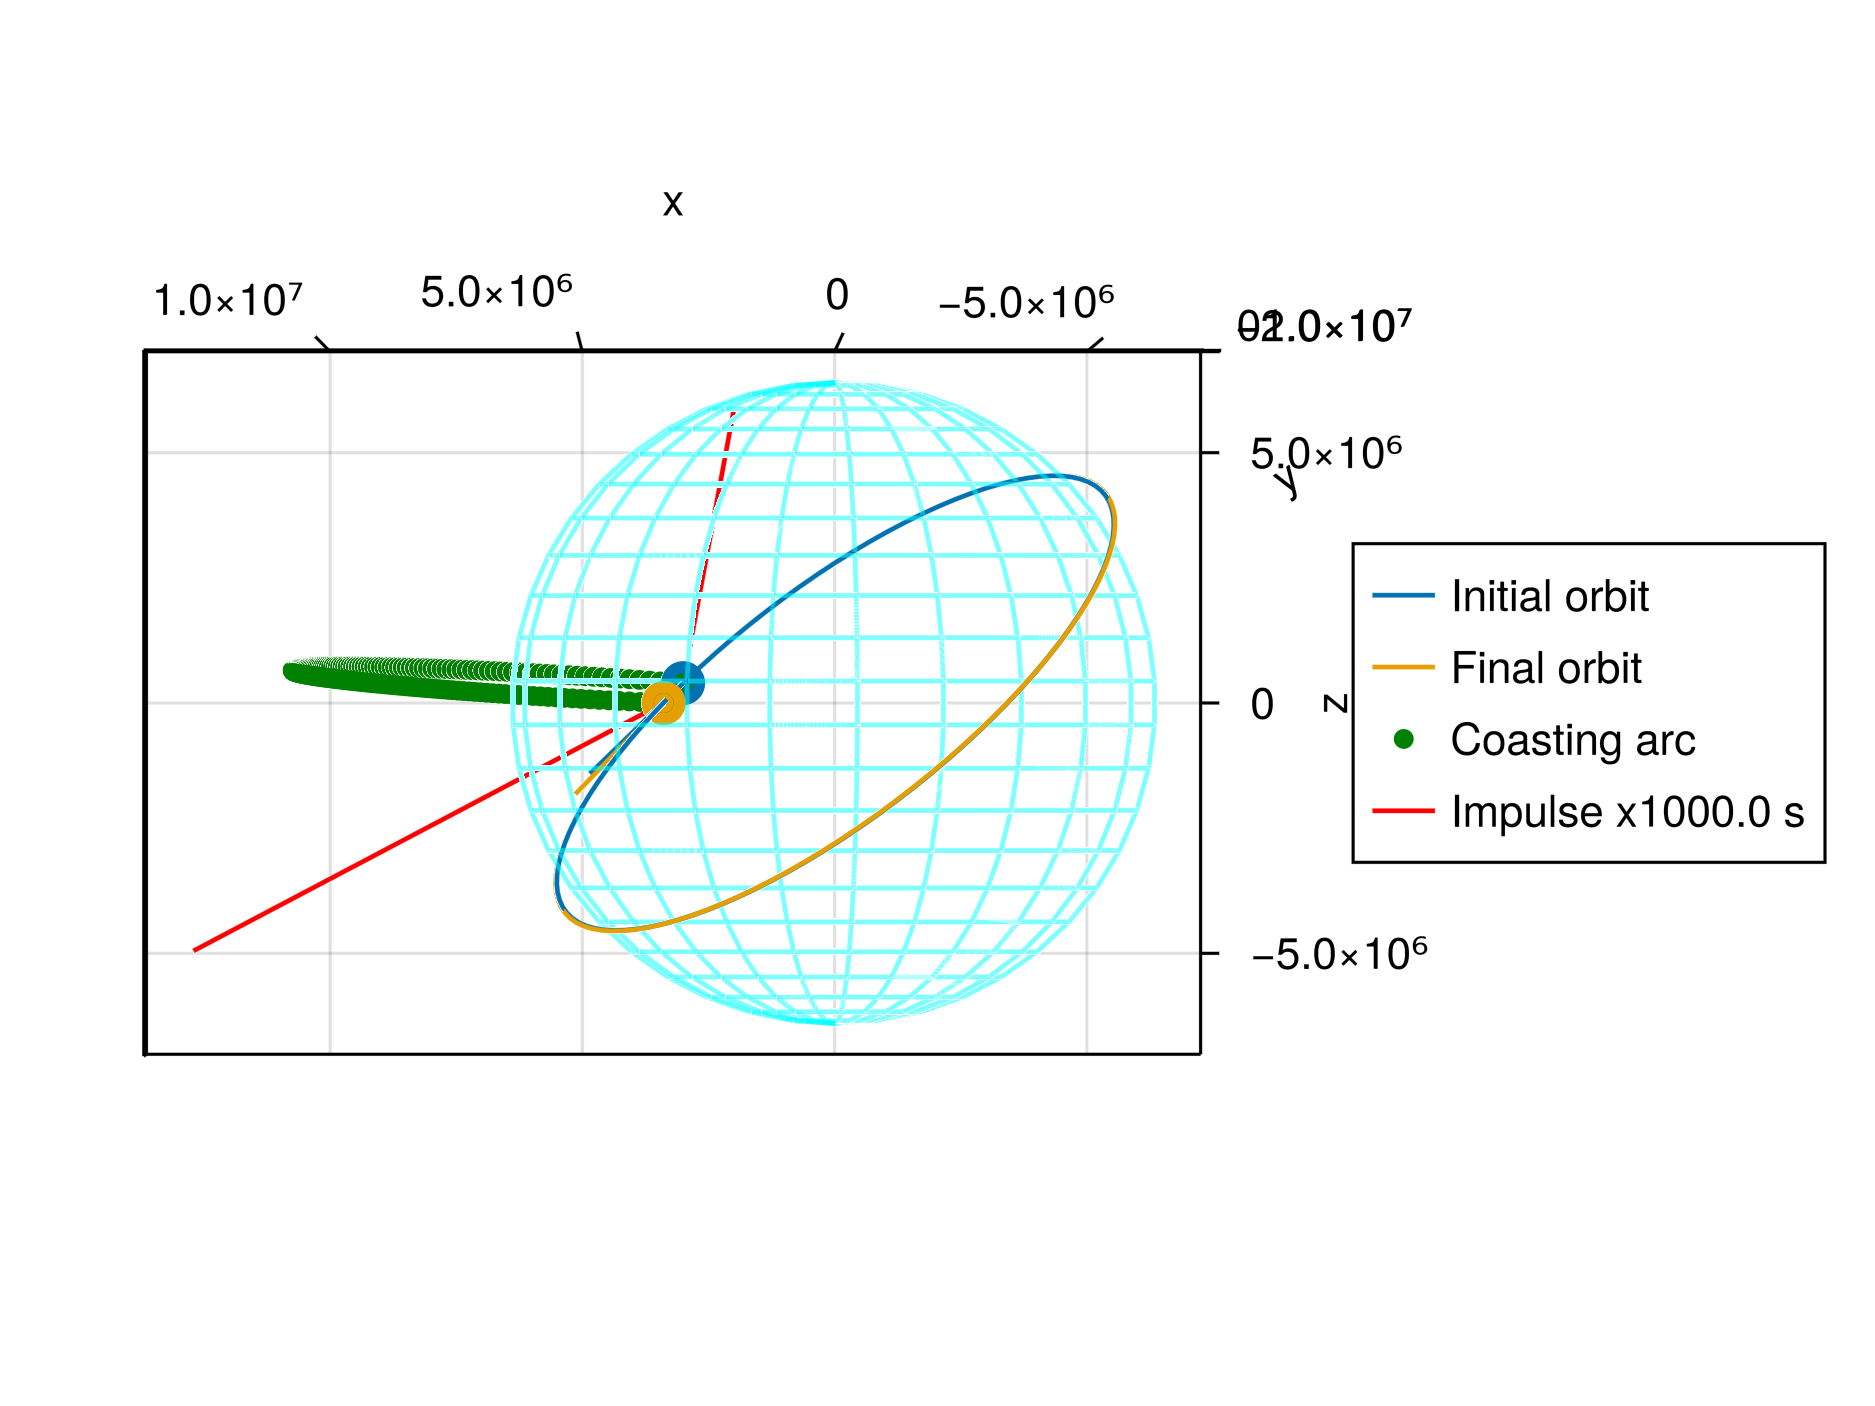
\includegraphics[width=\linewidth]{../results/two_body/ipv_noncop/ICI_y+.png}
        \caption{View from y+ axis.}
    \end{subfigure}
    \begin{subfigure}{0.49\linewidth}
        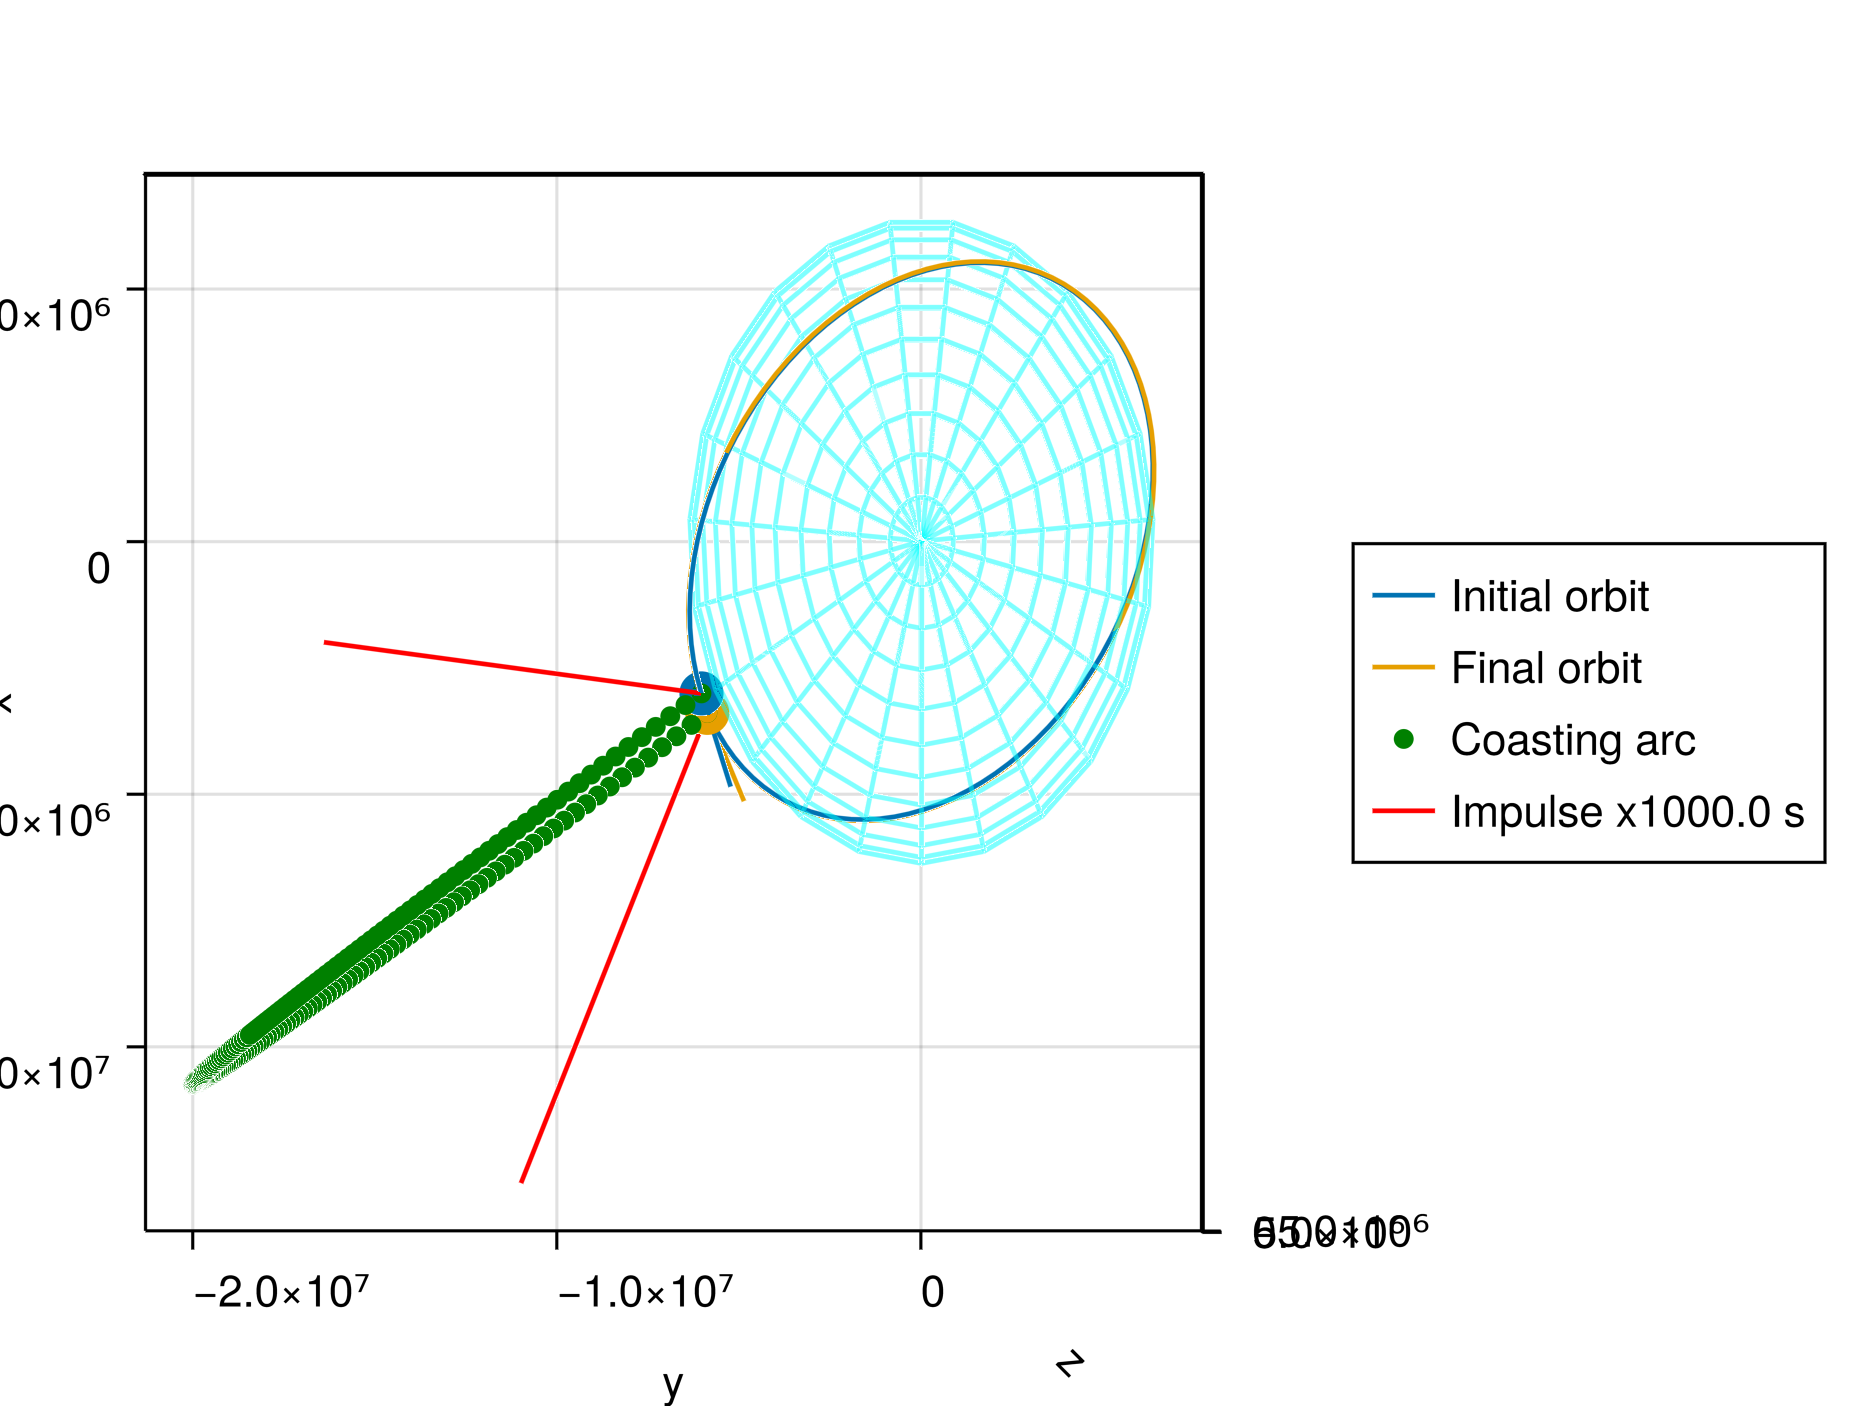
\includegraphics[width=\linewidth]{../results/two_body/ipv_noncop/ICI_z+.png}
        \caption{View from z+ axis.}
    \end{subfigure}
    \caption{Noncoplanar rendez-vous \texttt{ICI} maneuver 3D view and projections}
    \label{fig:tb_ncop_ICI_figs}
\end{figure}

Therefore, a \texttt{CICIC} maneuver case was optimized next. The maneuver's summary, primer vector trajectory, and spatial views can be seen in Table~\ref{tab:tb_ncop_CICIC_tab}, Figure~\ref{fig:tb_ncop_CICIC_pv} and Figure~\ref{fig:tb_ncop_CICIC_figs}. Now, the cost is much lower, and the trajectory is very close to the natural orbit of the satellite. However, the primer vector history violates the norm condition and shows that the addition of an extra impulse can lower the cost even further. 

% TB NCOP CICIC
\begin{table}[htpb]
    \centering
    \begin{tabular}{cccc} \toprule
    \multicolumn{2}{c}{\textbf{Maneuver type}} & \multicolumn{2}{c}{CICIC} \\ \midrule
    \(L\) (m) & \(T\) (s) & \(\varepsilon\) & \(\Delta x_{f}\) (m)    \\ \midrule
    6.7631e6          & 11107.158          & 1.00e-06                & 0.0                        \\ \midrule
    \(\max \lVert p \rVert\) & 3.327     & \textbf{Diagnostic}   & Add impulse        \\ \midrule
    \textbf{Impulse} & \(t\) (s) & \(\Delta v\) (m/s) & \(1 - p \cdot \hat{u}\) \\ \midrule
    1                 & 6644.30733          & 37.29252             & -0.0                    \\
    2                 & 10689.86179          & 16.20984             & -0.0                    \\\midrule
    \textbf{Total}   & 11107.1576          & 53.50237             &                     \\ \bottomrule   
    \end{tabular}
    \caption{Summary of optimization for two body noncoplanar \texttt{CICIC} rendez-vous.}
    \label{tab:tb_ncop_CICIC_tab}
\end{table}
% TB NCOP CICIC

\begin{figure}[htbp]
    \centering
    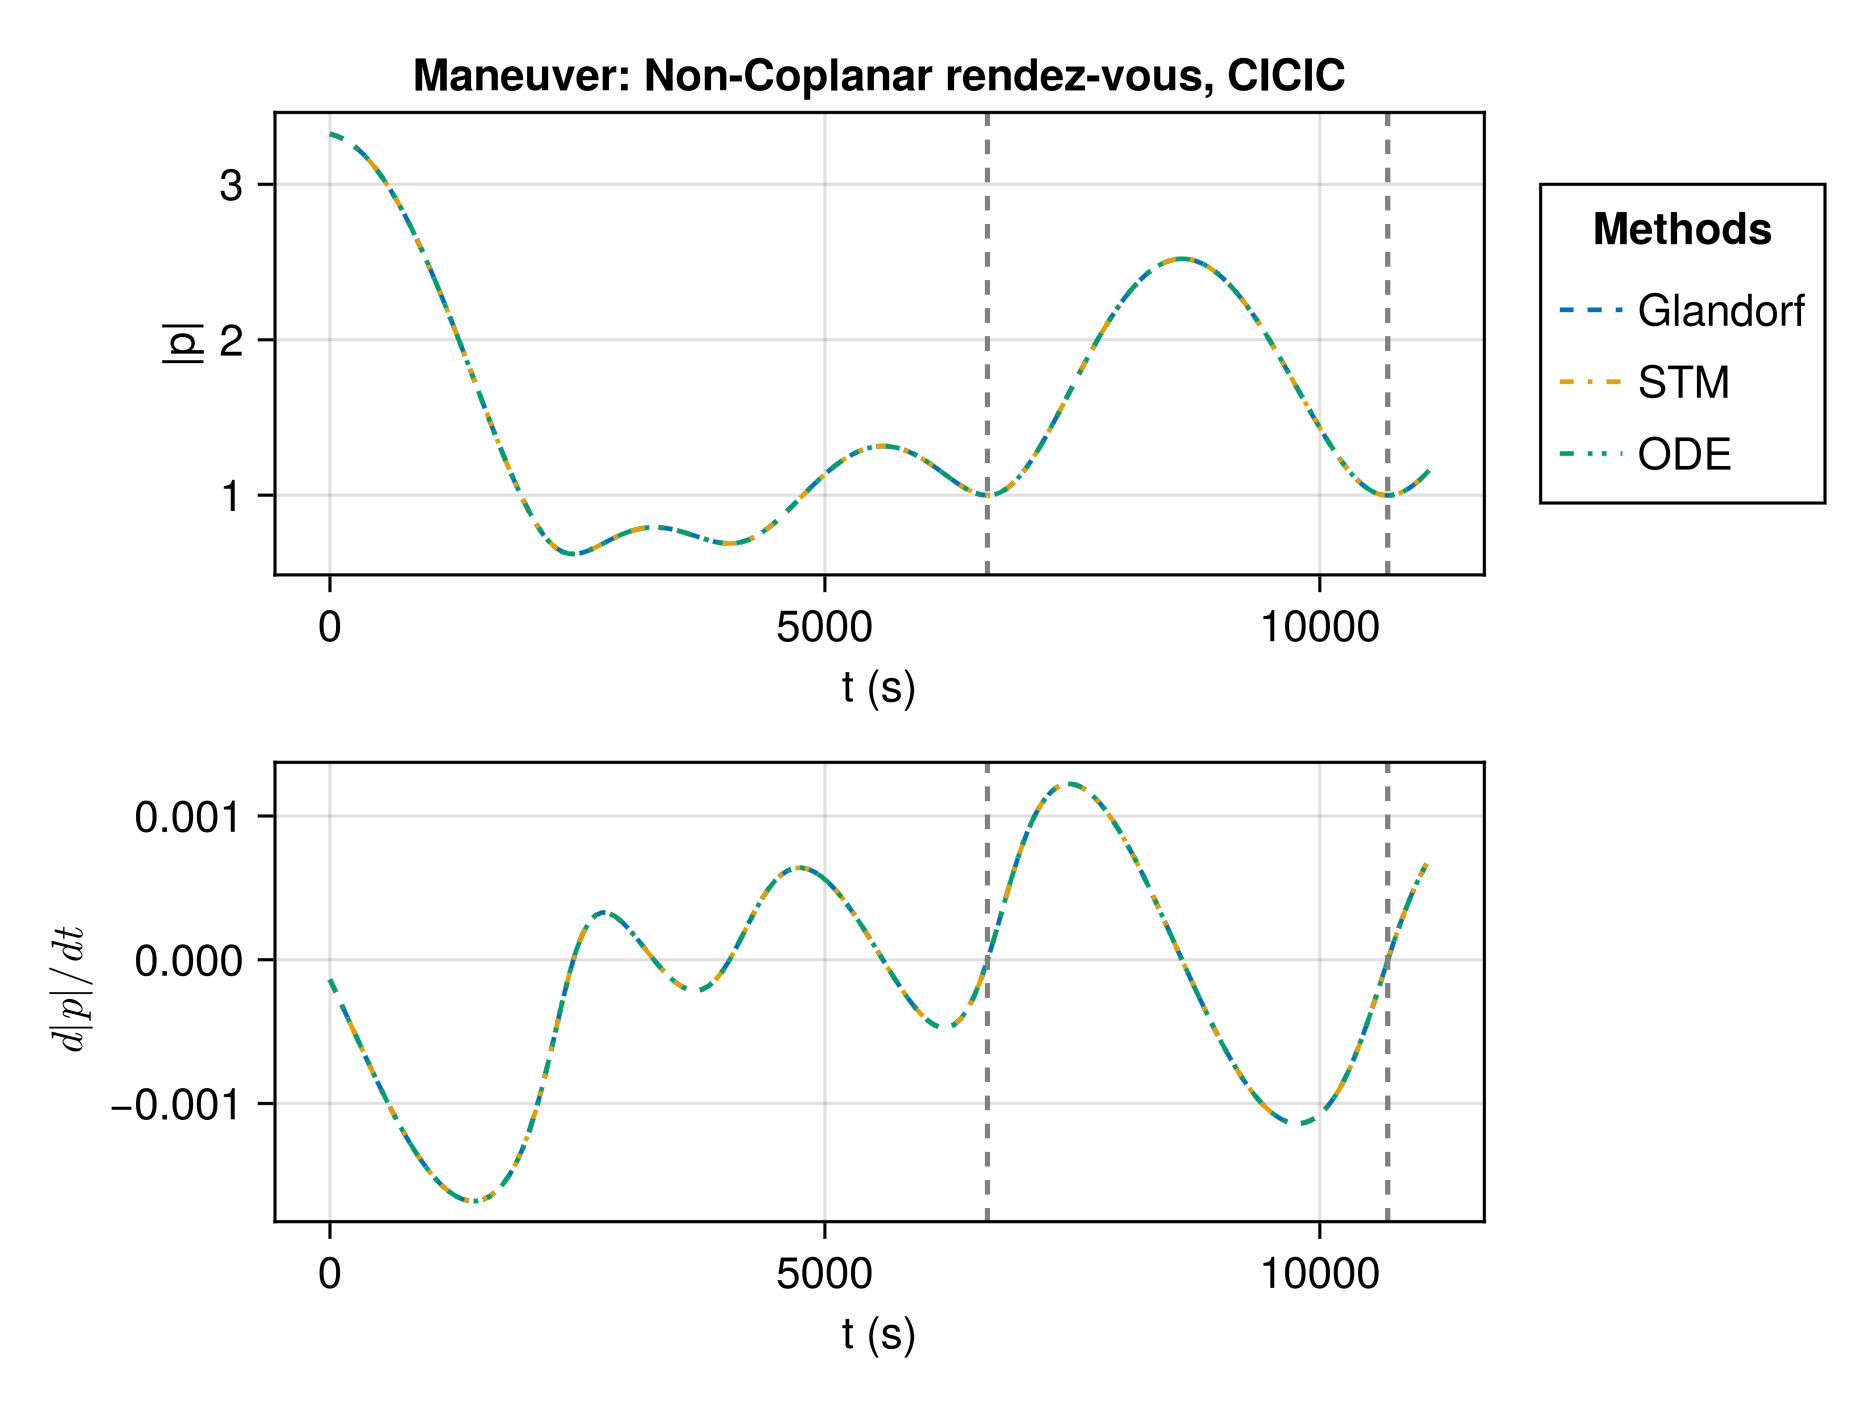
\includegraphics[width=\linewidth]{../results/two_body/ipv_noncop/CICIC_primer_vector.png}
    \caption{Primer vector trajectory for two body noncoplanar \texttt{CICIC} rendez-vous.}
    \label{fig:tb_ncop_CICIC_pv}
\end{figure}

\begin{figure}[htbp]
    \centering
    \begin{subfigure}{0.49\linewidth}
        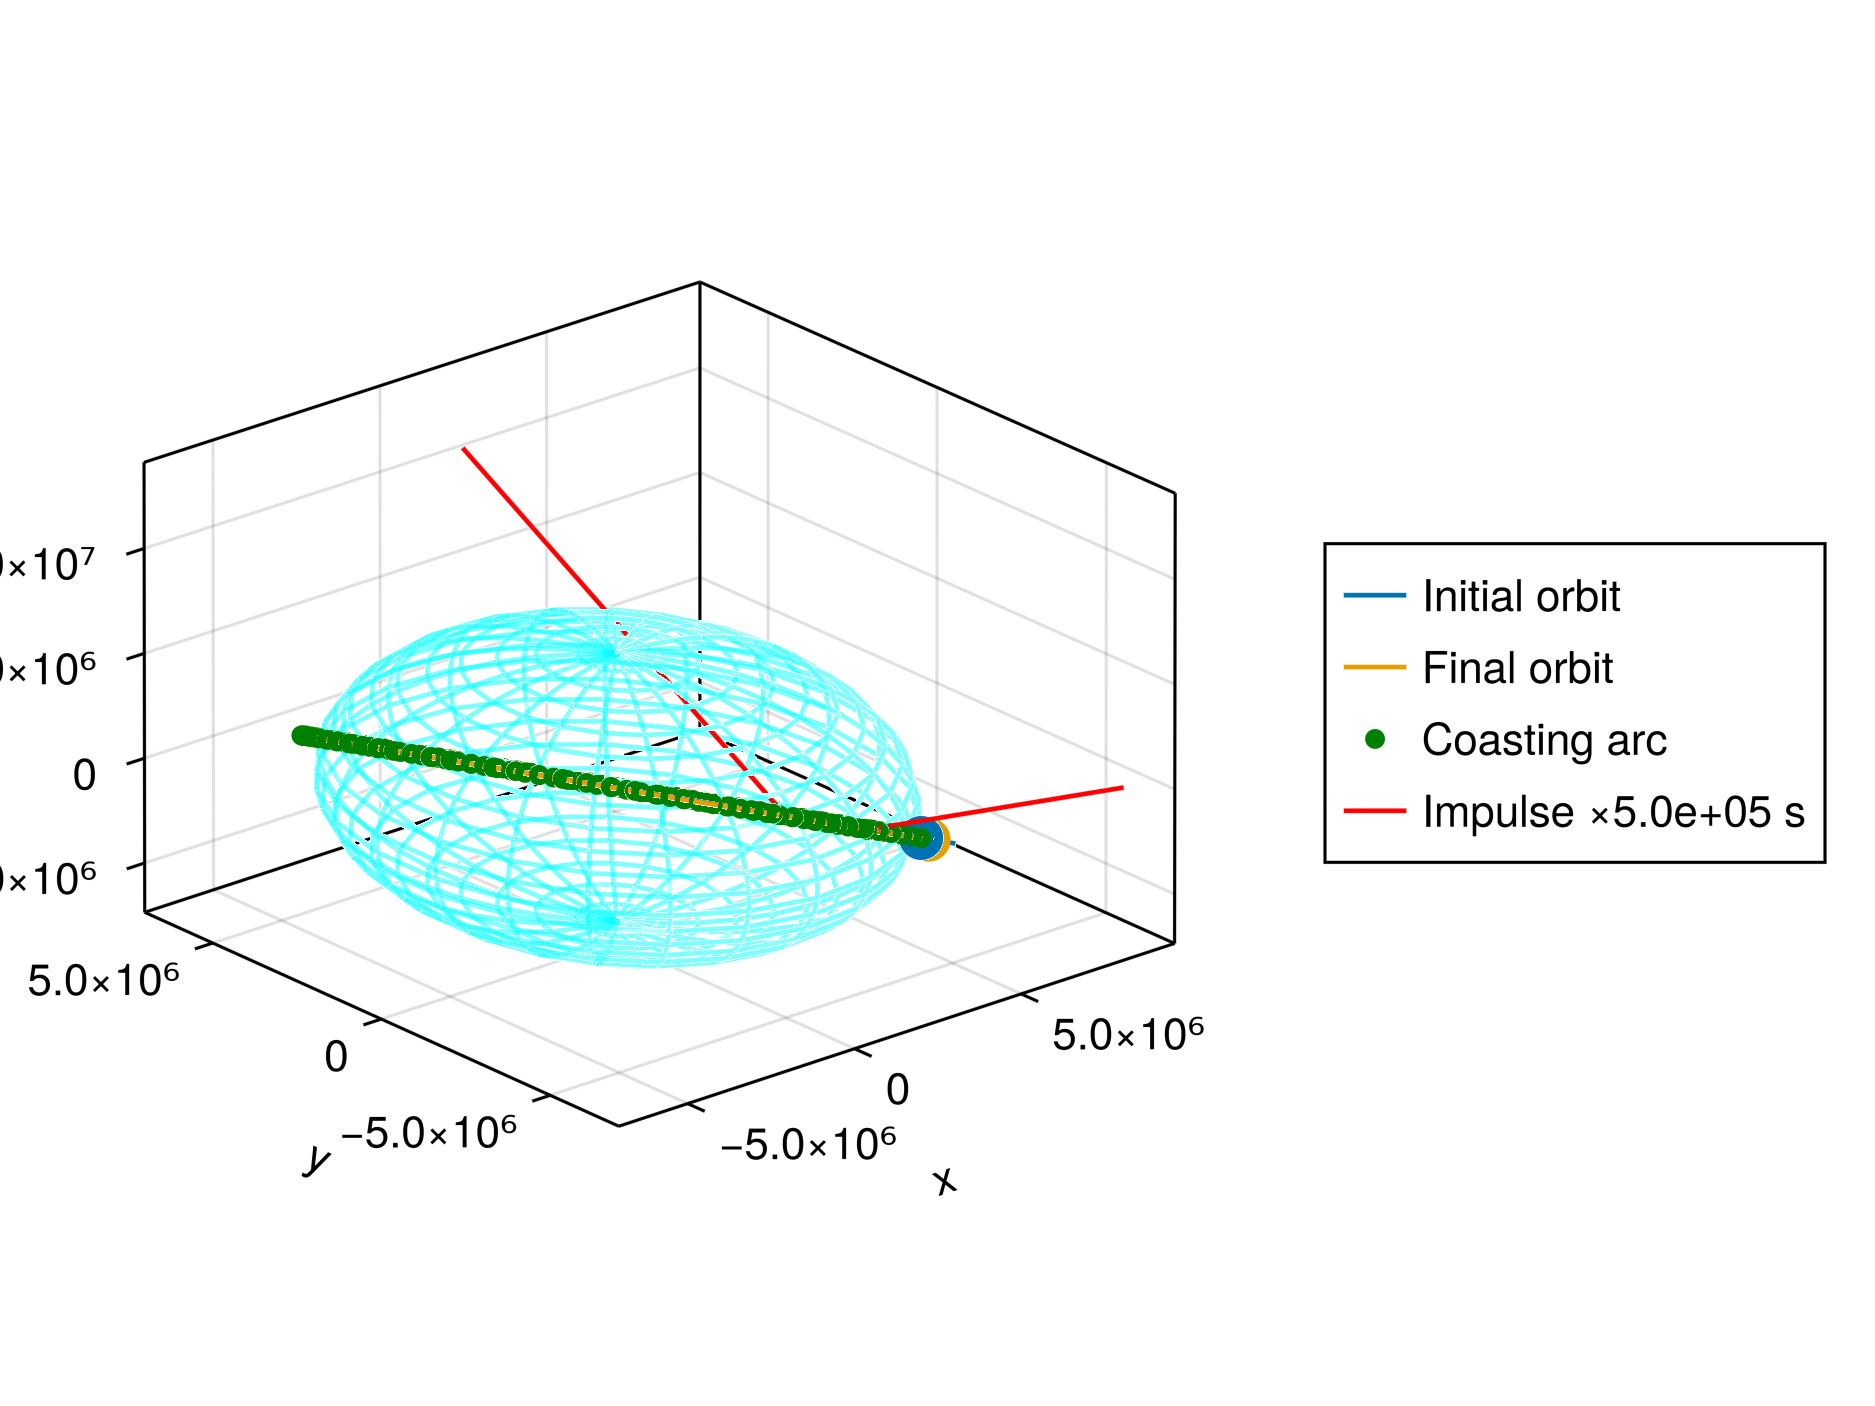
\includegraphics[width=\linewidth]{../results/two_body/ipv_noncop/CICIC_3d.png}
        \caption{3D view.}
    \end{subfigure}
    \begin{subfigure}{0.49\linewidth}
        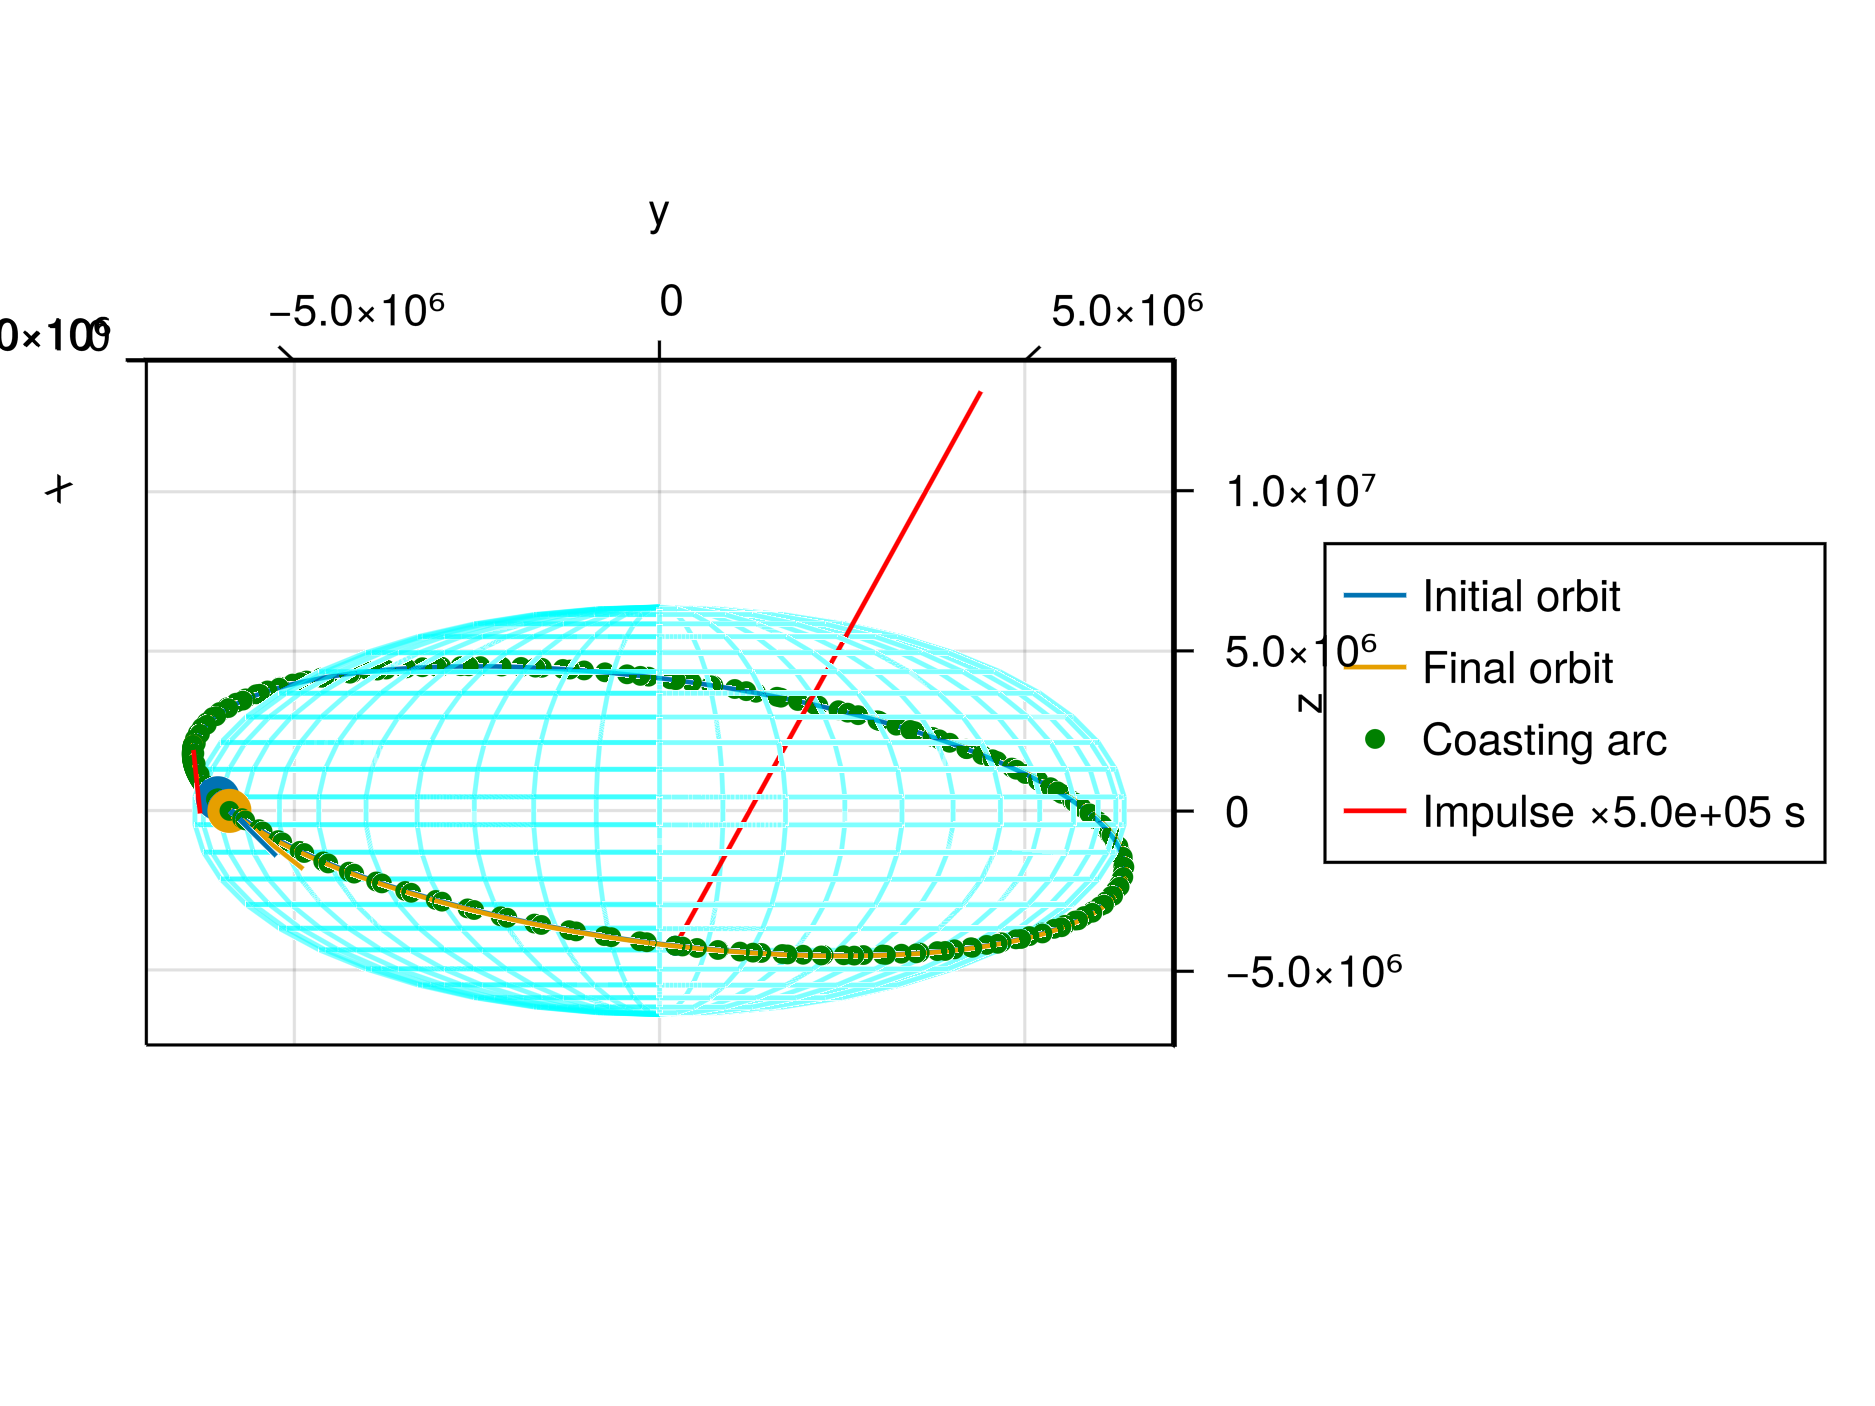
\includegraphics[width=\linewidth]{../results/two_body/ipv_noncop/CICIC_x+.png}
        \caption{View from x+ axis.}
    \end{subfigure}
    \begin{subfigure}{0.49\linewidth}
        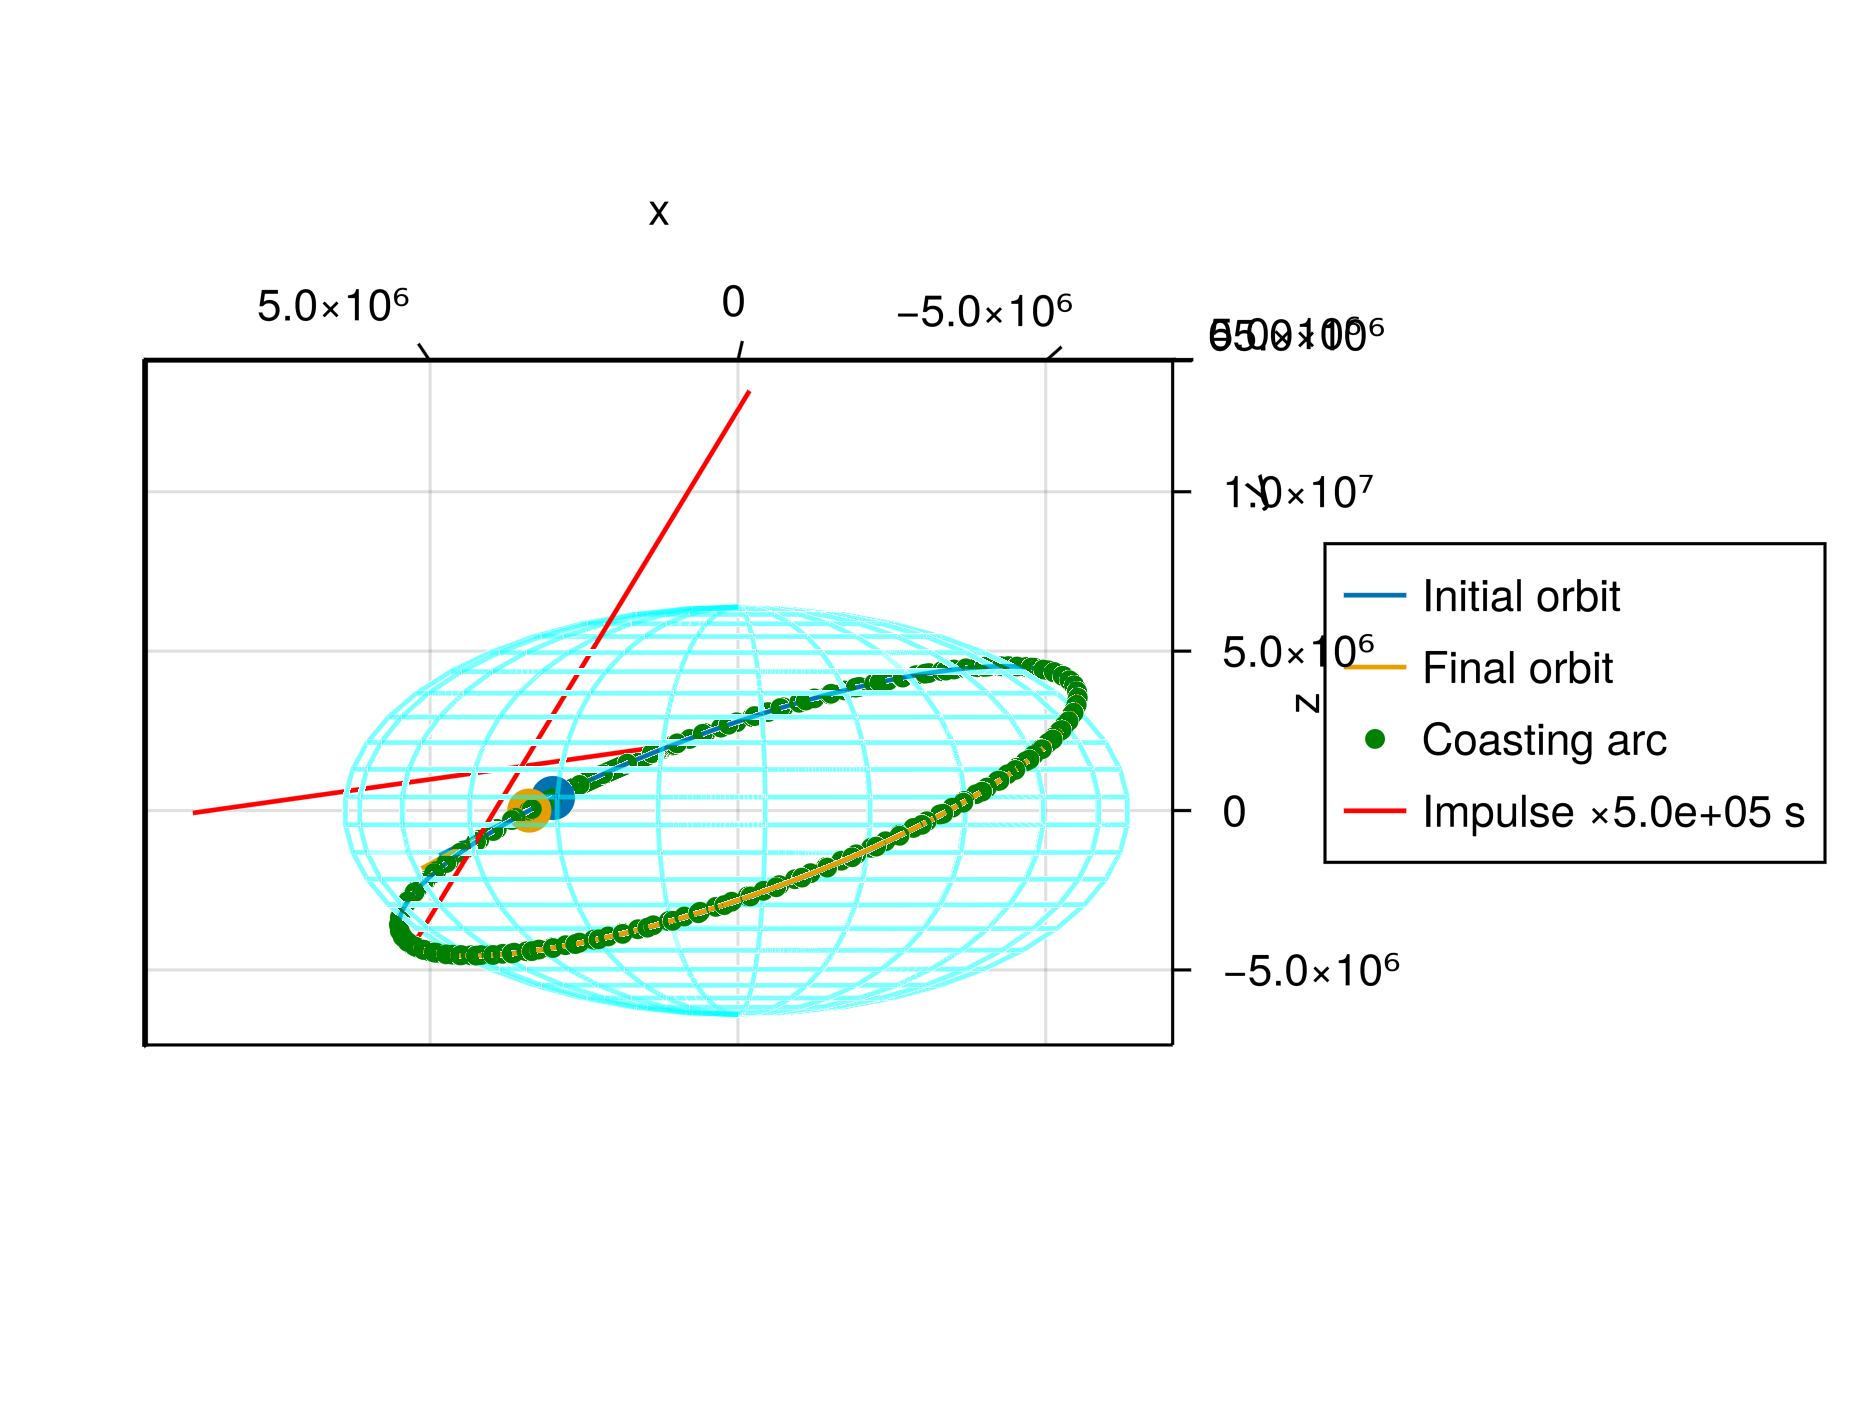
\includegraphics[width=\linewidth]{../results/two_body/ipv_noncop/CICIC_y+.png}
        \caption{View from y+ axis.}
    \end{subfigure}
    \begin{subfigure}{0.49\linewidth}
        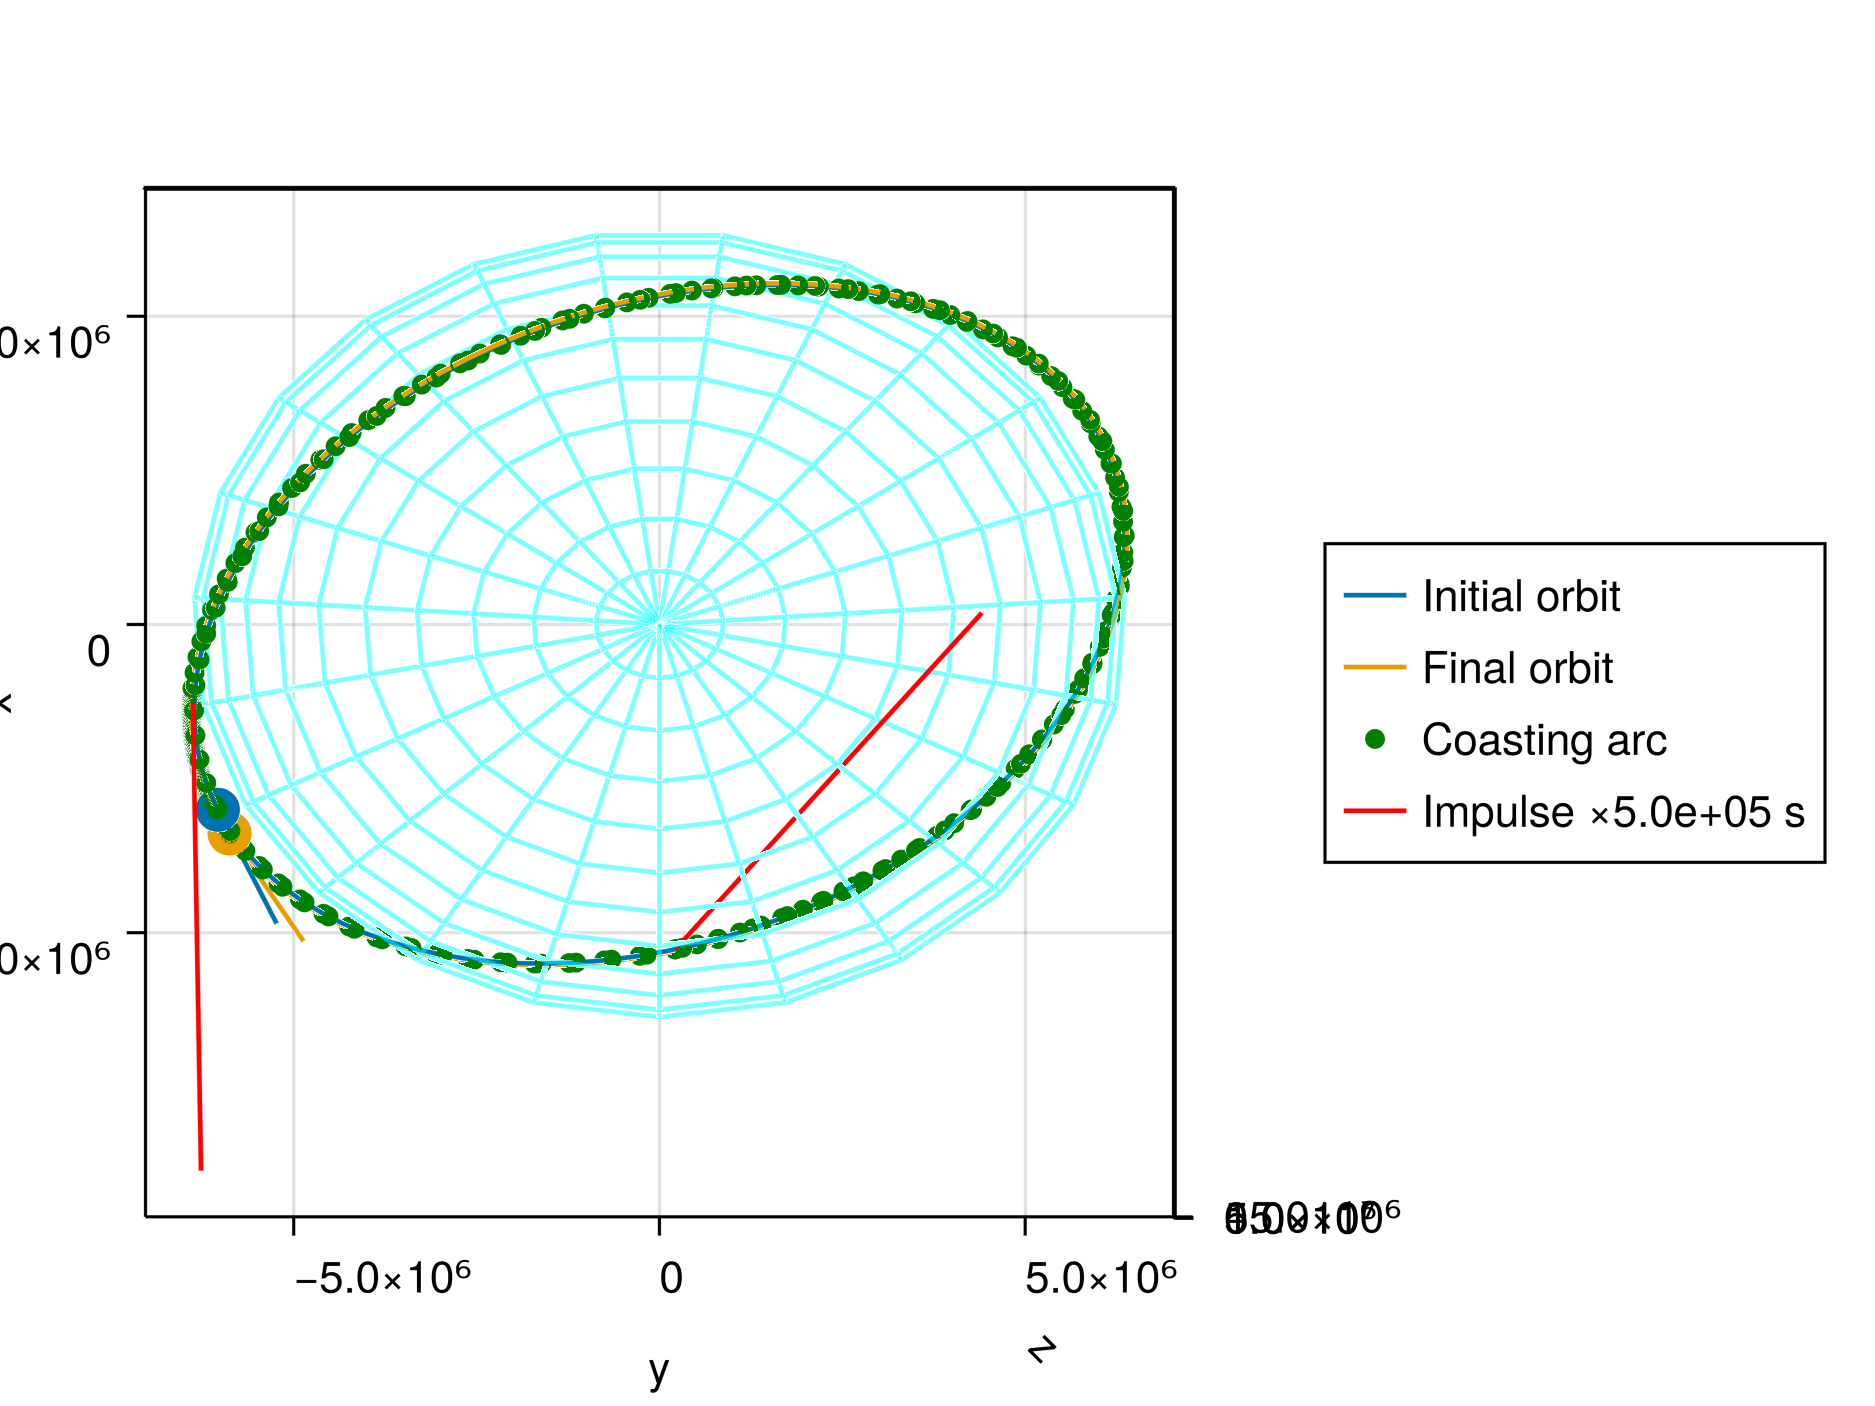
\includegraphics[width=\linewidth]{../results/two_body/ipv_noncop/CICIC_z+.png}
        \caption{View from z+ axis.}
    \end{subfigure}
    \caption{Noncoplanar rendez-vous \texttt{CICIC} maneuver 3D view and projections}
    \label{fig:tb_ncop_CICIC_figs}
\end{figure}

A \texttt{CICICIC} maneuver was searched based on the previous results. The spatial view is omitted since the trajectory closely resembles the natural orbit of the satellite. The maneuver summary and primer vector history are shown in Table~\ref{tab:tb_ncop_CICICIC_tab} and Figure~\ref{fig:tb_ncop_CICICIC_pv}. The addition of yet another impulse did reduce the \(\Delta v\) cost, but not as dramatically as the addition of initial and final coasts. Again, the maximum primer vector norm exceeds unity, which suggests another addition of impulse.

% TB C2C CICICIC
\begin{table}[htpb]
    \centering
    \begin{tabular}{cccc} \toprule
    \multicolumn{2}{c}{\textbf{Maneuver type}} & \multicolumn{2}{c}{CICICIC} \\ \midrule
    \(L\) (m) & \(T\) (s) & \(\varepsilon\) & \(\Delta x_{f}\) (m)    \\ \midrule
    6.7631e6          & 11107.158          & 1.00e-05                & 0.0                        \\ \midrule
    \(\max \lVert p \rVert\) & 1.9638     & \textbf{Diagnostic}   & Add impulse        \\ \midrule
    \textbf{Impulse} & \(t\) (s) & \(\Delta v\) (m/s) & \(1 - p \cdot \hat{u}\) \\ \midrule
    1                 & 3370.1071          & 11.76294             & -0.0                    \\
    2                 & 6774.61652          & 10.56494             & 0.0                    \\
    3                 & 9176.42663          & 20.74554             & -0.0                    \\\midrule
    \textbf{Total}   & 11107.1576          & 43.07342             &                     \\ \bottomrule   
    \end{tabular}
    \caption{Summary of optimization for two body noncoplanar \texttt{CICICIC} rendez-vous.}
    \label{tab:tb_ncop_CICICIC_tab}
\end{table}
% TB C2C CICICIC

\begin{figure}[htbp]
    \centering
    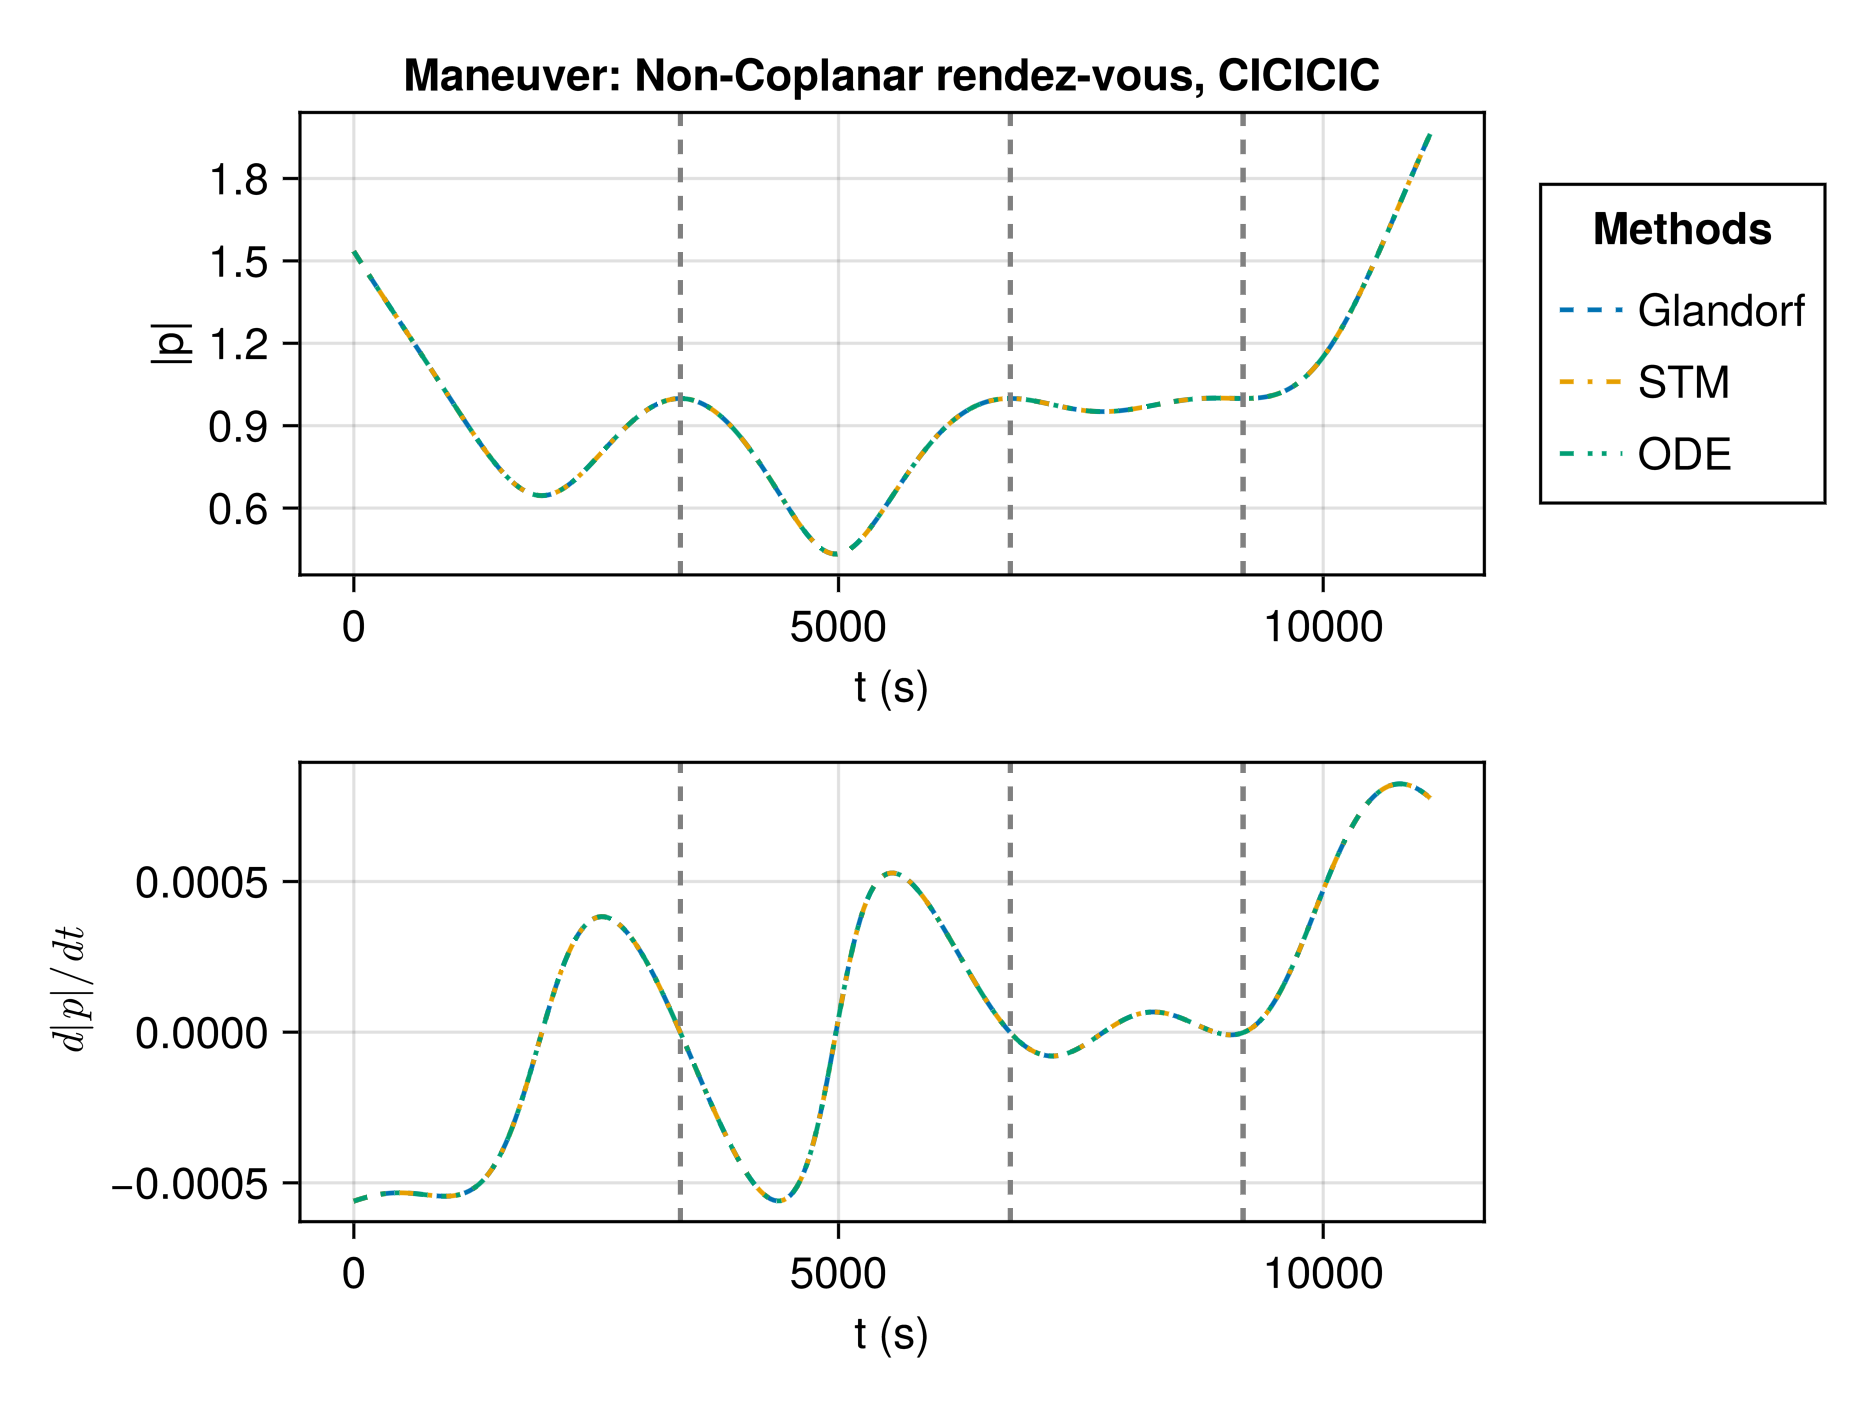
\includegraphics[width=\linewidth]{../results/two_body/ipv_noncop/CICICIC_primer_vector.png}
    \caption{Primer vector trajectory for two body noncoplanar \texttt{CICICIC} rendez-vous.}
    \label{fig:tb_ncop_CICICIC_pv}
\end{figure}

Finally, the addition of a fourth impulse attains the primer vector necessary conditions, as attested in its trajectory in Figure~\ref{fig:tb_ncop_CICICICIC_pv} and its summary in Table~\ref{tab:tb_ncop_CICICICIC_tab}. A small error of \(0.4\%\) has been allowed in the primer vector norm, which is small enough that only a very small fifth impulse would marginally reduce cost, for no tangible algorithmic gain. The final velocity cost is well within feasible for many spatial applications, with the caveat that the spacecraft must be correctly pointed at four points in time. 

\begin{table}[htpb]
    \centering
    \begin{tabular}{cccc} \toprule
    \multicolumn{2}{c}{\textbf{Maneuver type}} & \multicolumn{2}{c}{CICICICIC} \\ \midrule
    \(L\) (m) & \(T\) (s) & \(\varepsilon\) & \(\Delta x_{f}\) (m)    \\ \midrule
    6.7631e6          & 11107.158          & 1.00e-05                & 0.04983                        \\ \midrule
    \(\max \lVert p \rVert\) & 1.0046     & \textbf{Diagnostic}   & Add impulse        \\ \midrule
    \textbf{Impulse} & \(t\) (s) & \(\Delta v\) (m/s) & \(1 - p \cdot \hat{u}\) \\ \midrule
    1                 & 0.00394          & 3.58823             & 0.0                    \\
    2                 & 6724.60052          & 9.34687             & -0.0                    \\
    3                 & 9217.50949          & 15.01486             & -0.0                    \\
    4                 & 11107.15747          & 8.19599             & -0.0                    \\\midrule
    \textbf{Total}   & 11107.1576          & 36.14596             &                     \\ \bottomrule   
    \end{tabular}
    \caption{Summary of optimization for two body noncoplanar \texttt{CICICICIC} rendez-vous.}
    \label{tab:tb_ncop_CICICICIC_tab}
\end{table}

\begin{figure}[htbp]
    \centering
    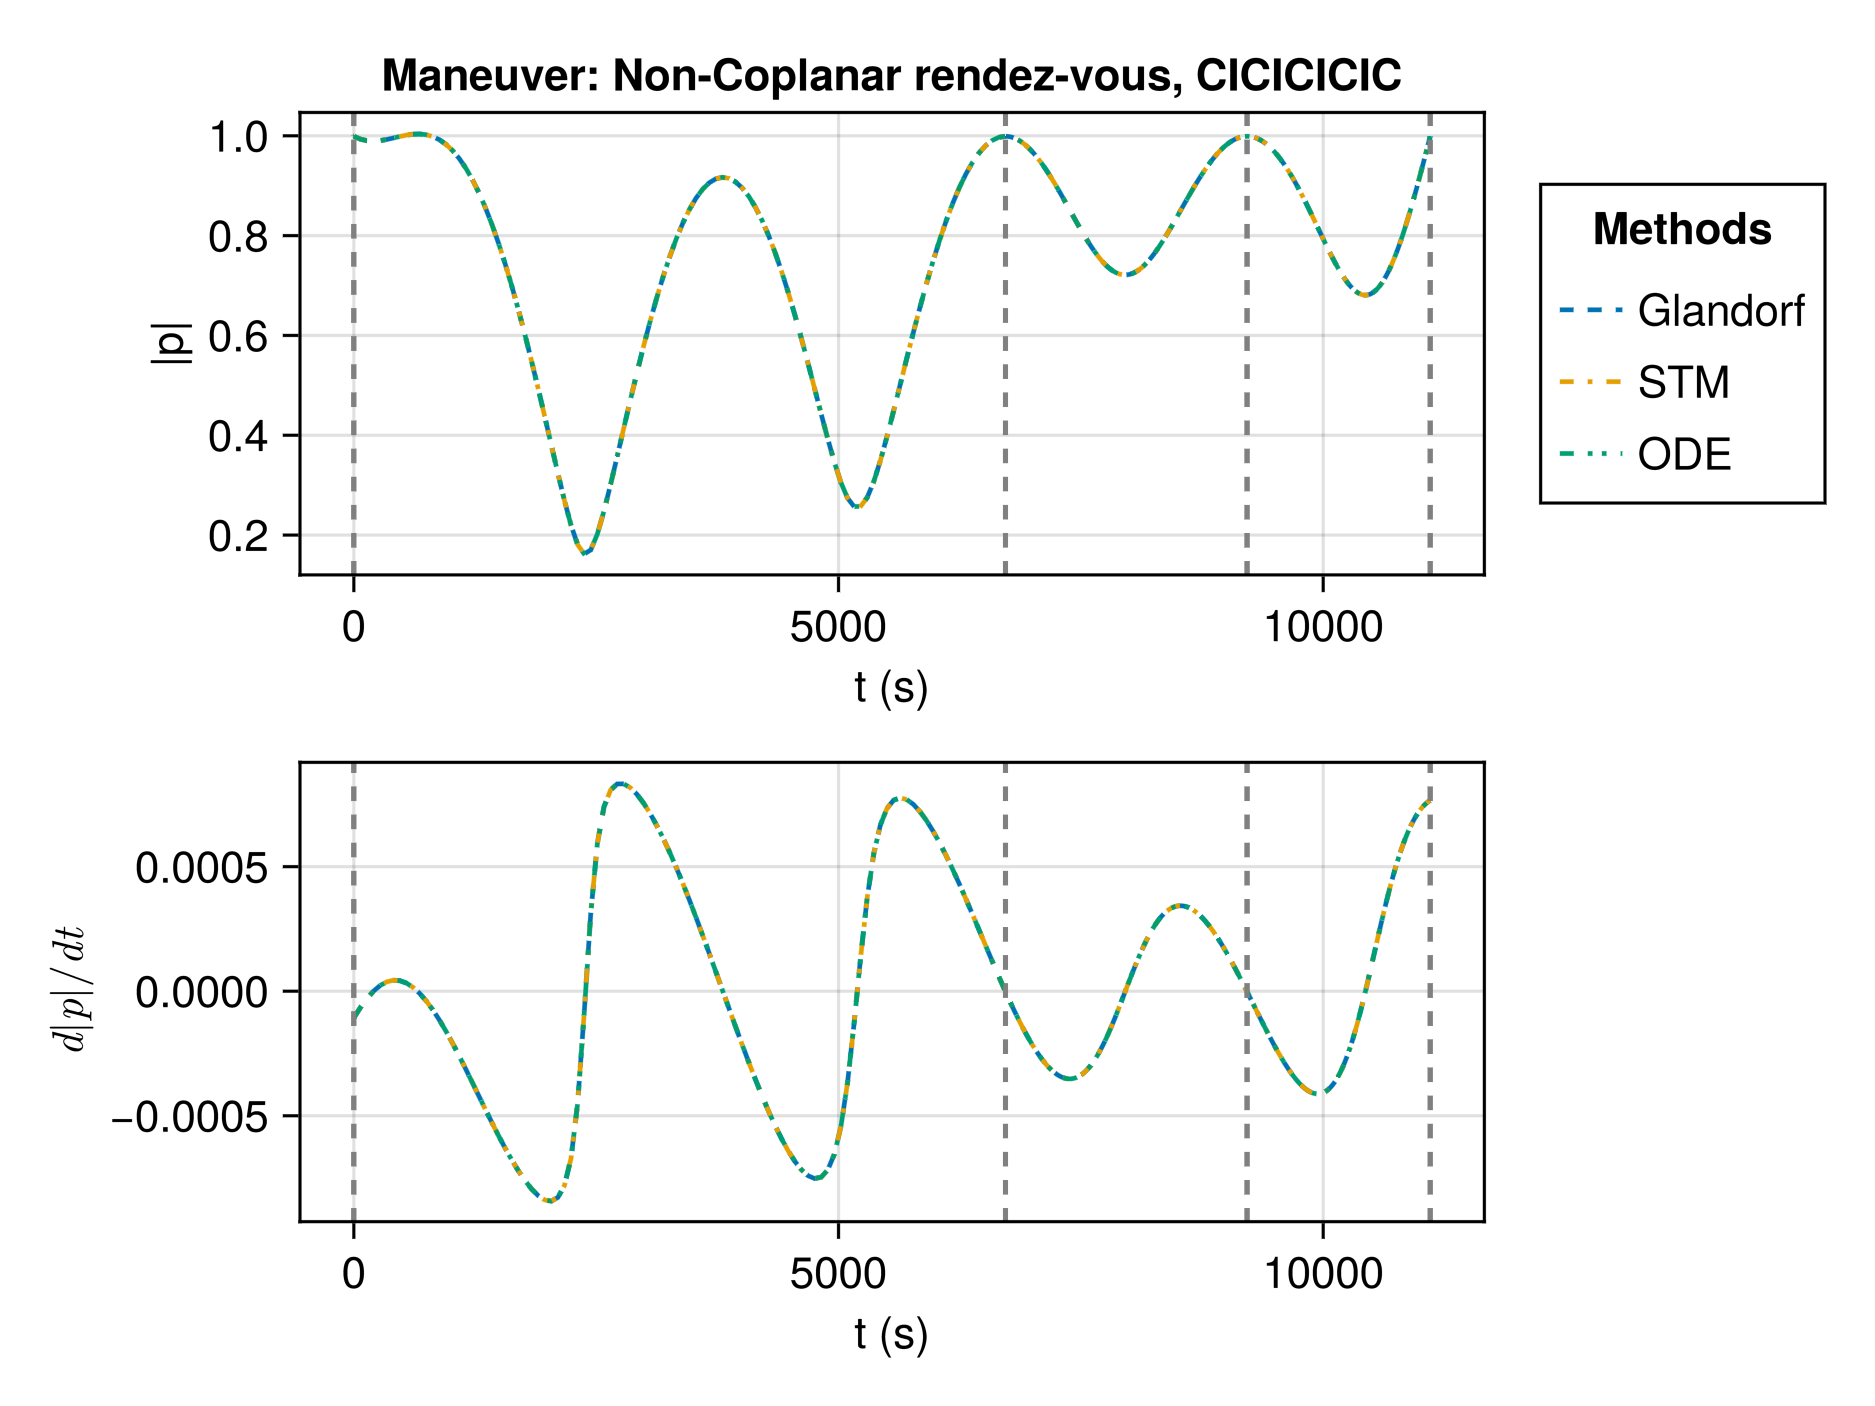
\includegraphics[width=\linewidth]{../results/two_body/ipv_noncop/CICICICIC_primer_vector.png}
    \caption{Primer vector trajectory for two body noncoplanar \texttt{CICICICIC} rendez-vous.}
    \label{fig:tb_ncop_CICICICIC_pv}
\end{figure}

\newpage
\FloatBarrier
\section{J2 Model}

Optimized maneuvers are presented for the aforementioned scenarios under the J2 model introduced previously. Under this model, only the STM and ODE methods correctly calculate primer vector trajectories, and both will be presented for all cases.

\subsection{Circle to Circle}

TODO put texttt in tables

The simple circle to circle rendez-vous case was first optimized with a \texttt{ICI} maneuver, with results that can be seen in Table~\ref{tab:j2_c2c_ICI_tab}, Figure~\ref{fig:j2_c2c_ICI_pv} and Figure~\ref{fig:j2_c2c_ICI_figs}. To analyze the polar trajectory that was found, first it is worth mentioning that orbital trajectories under the J2 model are, in general, not planar, which means that the two-body Hohmann transfer is impossible with this model. The only planar orbits are perfectly equatorial and perfectly polar orbits and, due to the inclination of the orbits' being greater than \(45^\circ\), the polar orbit is the best solution. It is vastly different to the two-body \texttt{ICI} solution, which shows the J2 perturbations are very relevant to LEO orbits, even in small time frames. However, the primer vector trajectory shows that the necessary conditions are not satisfied and, in particular, endpoint derivatives are positive and negative, respectively, which shows that the \texttt{ICI} solution is not even a local optimum in the space of \texttt{CICIC} solutions. Therefore, adding initial and final coasts should reduce the very large cost of this solution.

\begin{table}[htpb]
    \centering
    \begin{tabular}{cccc} \toprule
    \multicolumn{2}{c}{\textbf{Maneuver type}} & \multicolumn{2}{c}{ICI} \\ \midrule
    \(L\) (m) & \(T\) (s) & \(\varepsilon\) & \(\Delta x_{f}\) (m)    \\ \midrule
    8.0e6          & 1.0          & 1.00e-05                & 0.49713                        \\ \midrule
    \(\max \lVert p \rVert\) & 563.46     & \textbf{Diagnostic}   & Initial + Final coast        \\ \midrule
    \textbf{Impulse} & \(t\) (s) & \(\Delta v\) (m/s) & \(1 - p \cdot \hat{u}\) \\ \midrule
    1                 & 0.0          & 5209.47789             & -0.0                    \\
    2                 & 3560.54079          & 4318.71793             & -0.0                    \\\midrule
    \textbf{Total}   & 3560.54079          & 9528.19582             &                     \\ \bottomrule   
    \end{tabular}
    \caption{Summary of optimization for J2 circle to circle \texttt{ICI} rendez-vous.}
    \label{tab:j2_c2c_ICI_tab}
\end{table}

\begin{figure}[htbp]
    \centering
    \begin{subfigure}{0.49\linewidth}
        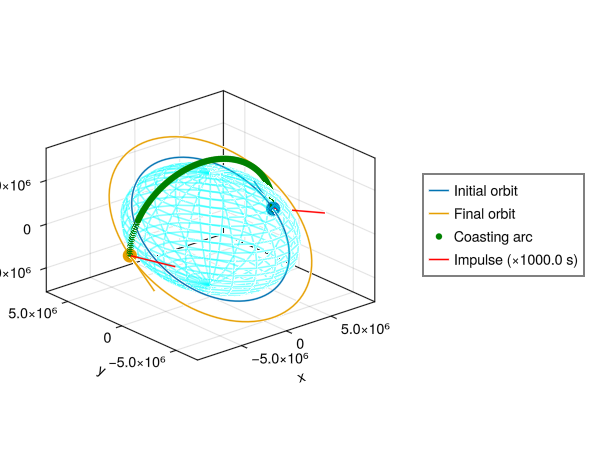
\includegraphics[width=\linewidth]{../results/j2/hohmann/ICI_3d.png}
        \caption{3D view.}
    \end{subfigure}
    \begin{subfigure}{0.49\linewidth}
        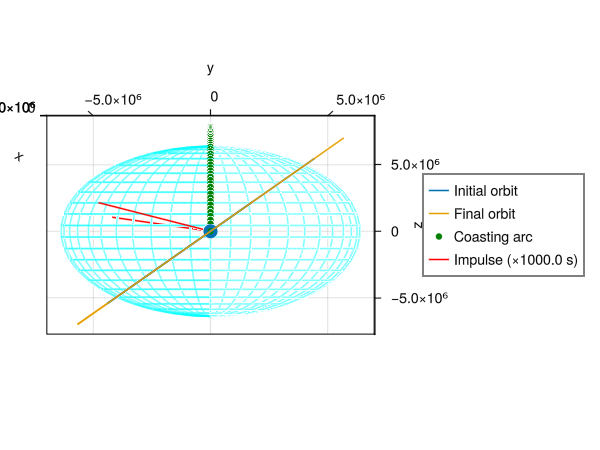
\includegraphics[width=\linewidth]{../results/j2/hohmann/ICI_x+.png}
        \caption{View from x+ axis.}
    \end{subfigure}
    \begin{subfigure}{0.49\linewidth}
        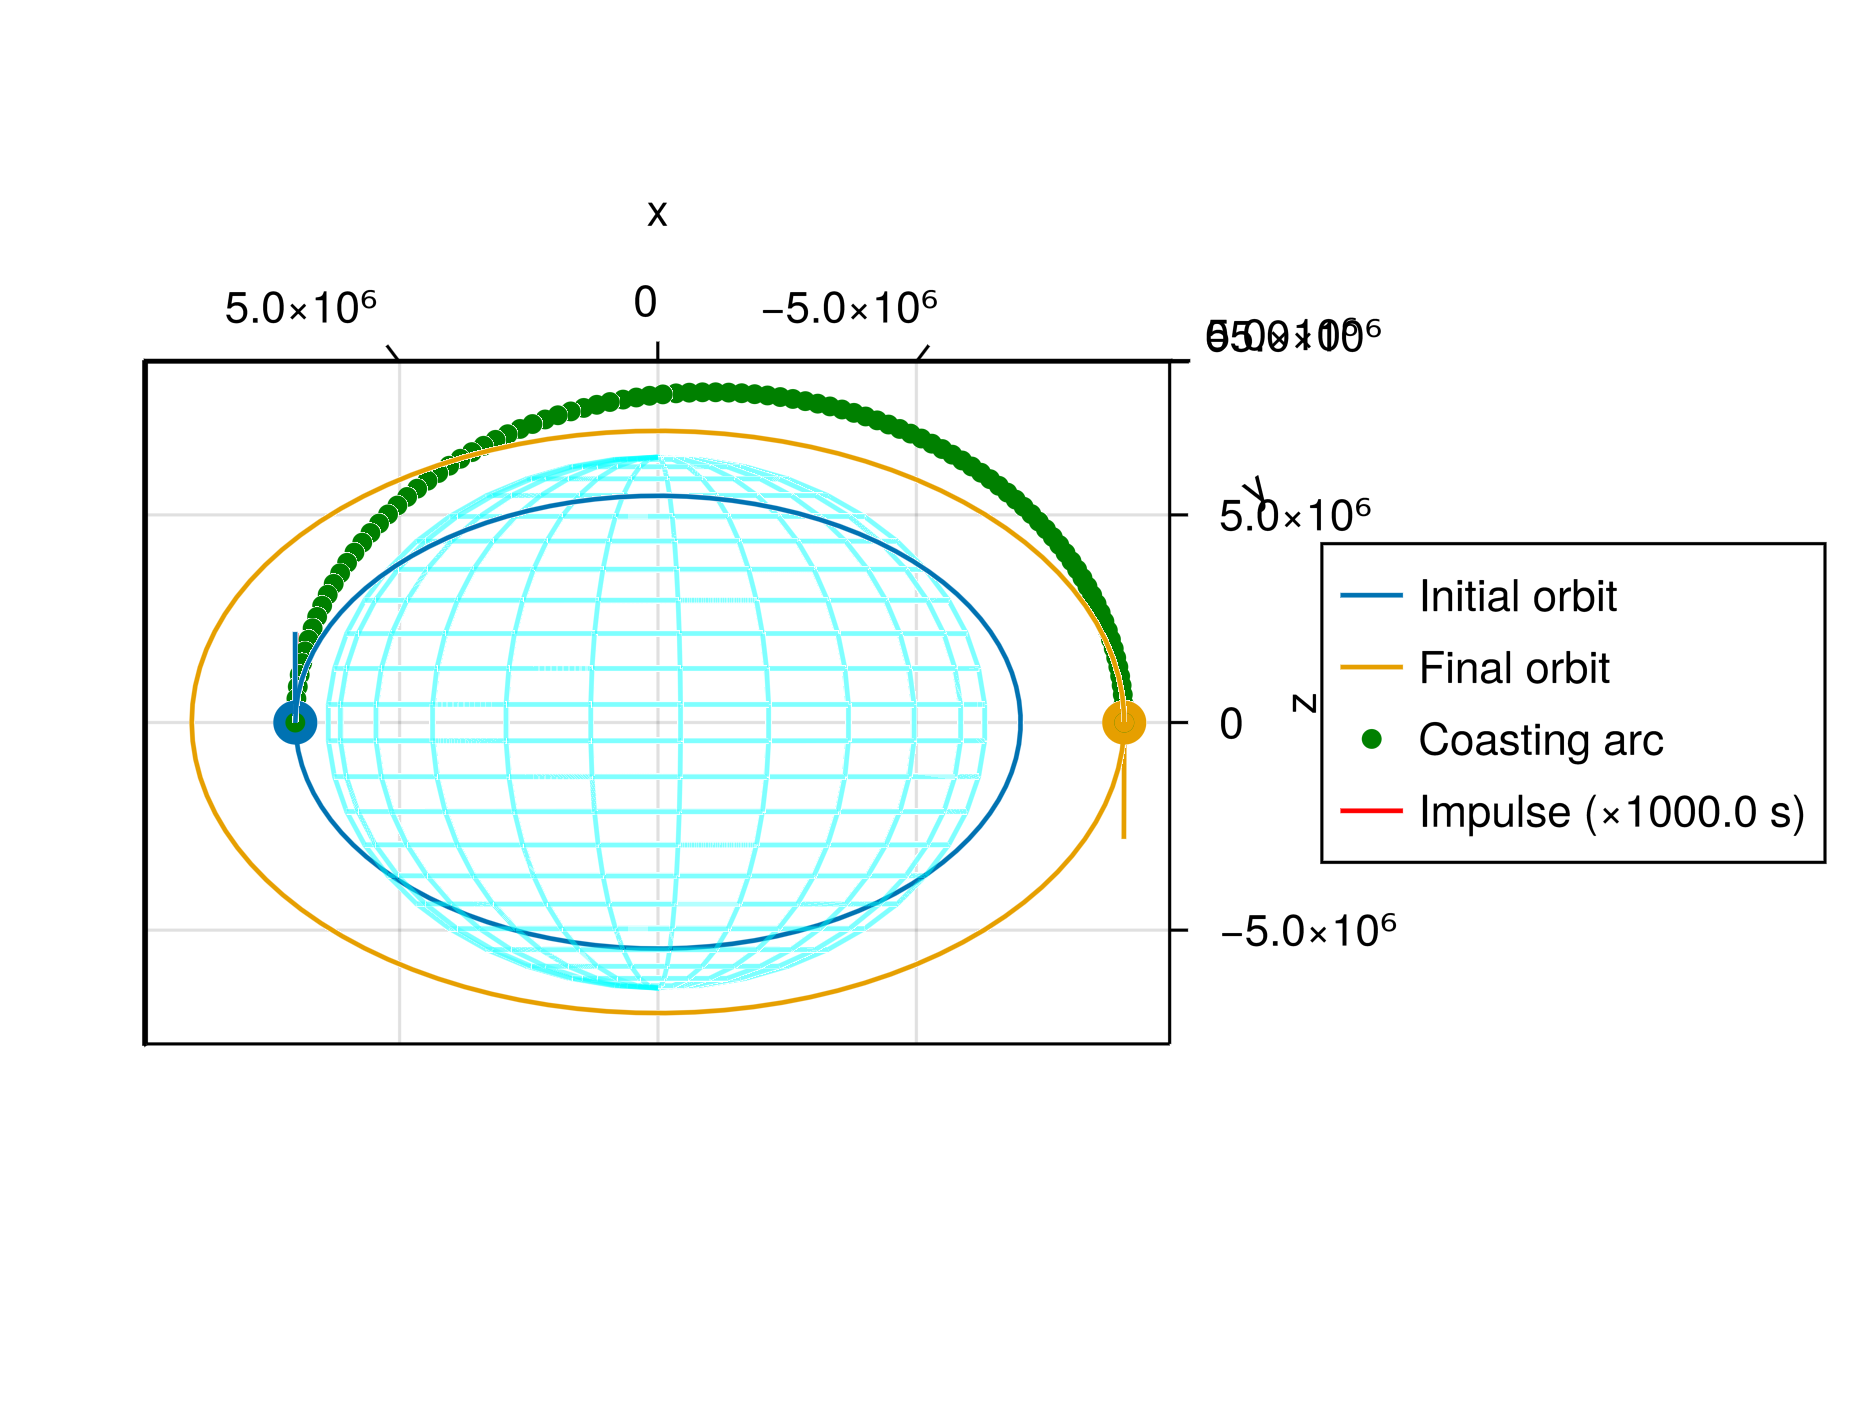
\includegraphics[width=\linewidth]{../results/j2/hohmann/ICI_y+.png}
        \caption{View from y+ axis.}
    \end{subfigure}
    \begin{subfigure}{0.49\linewidth}
        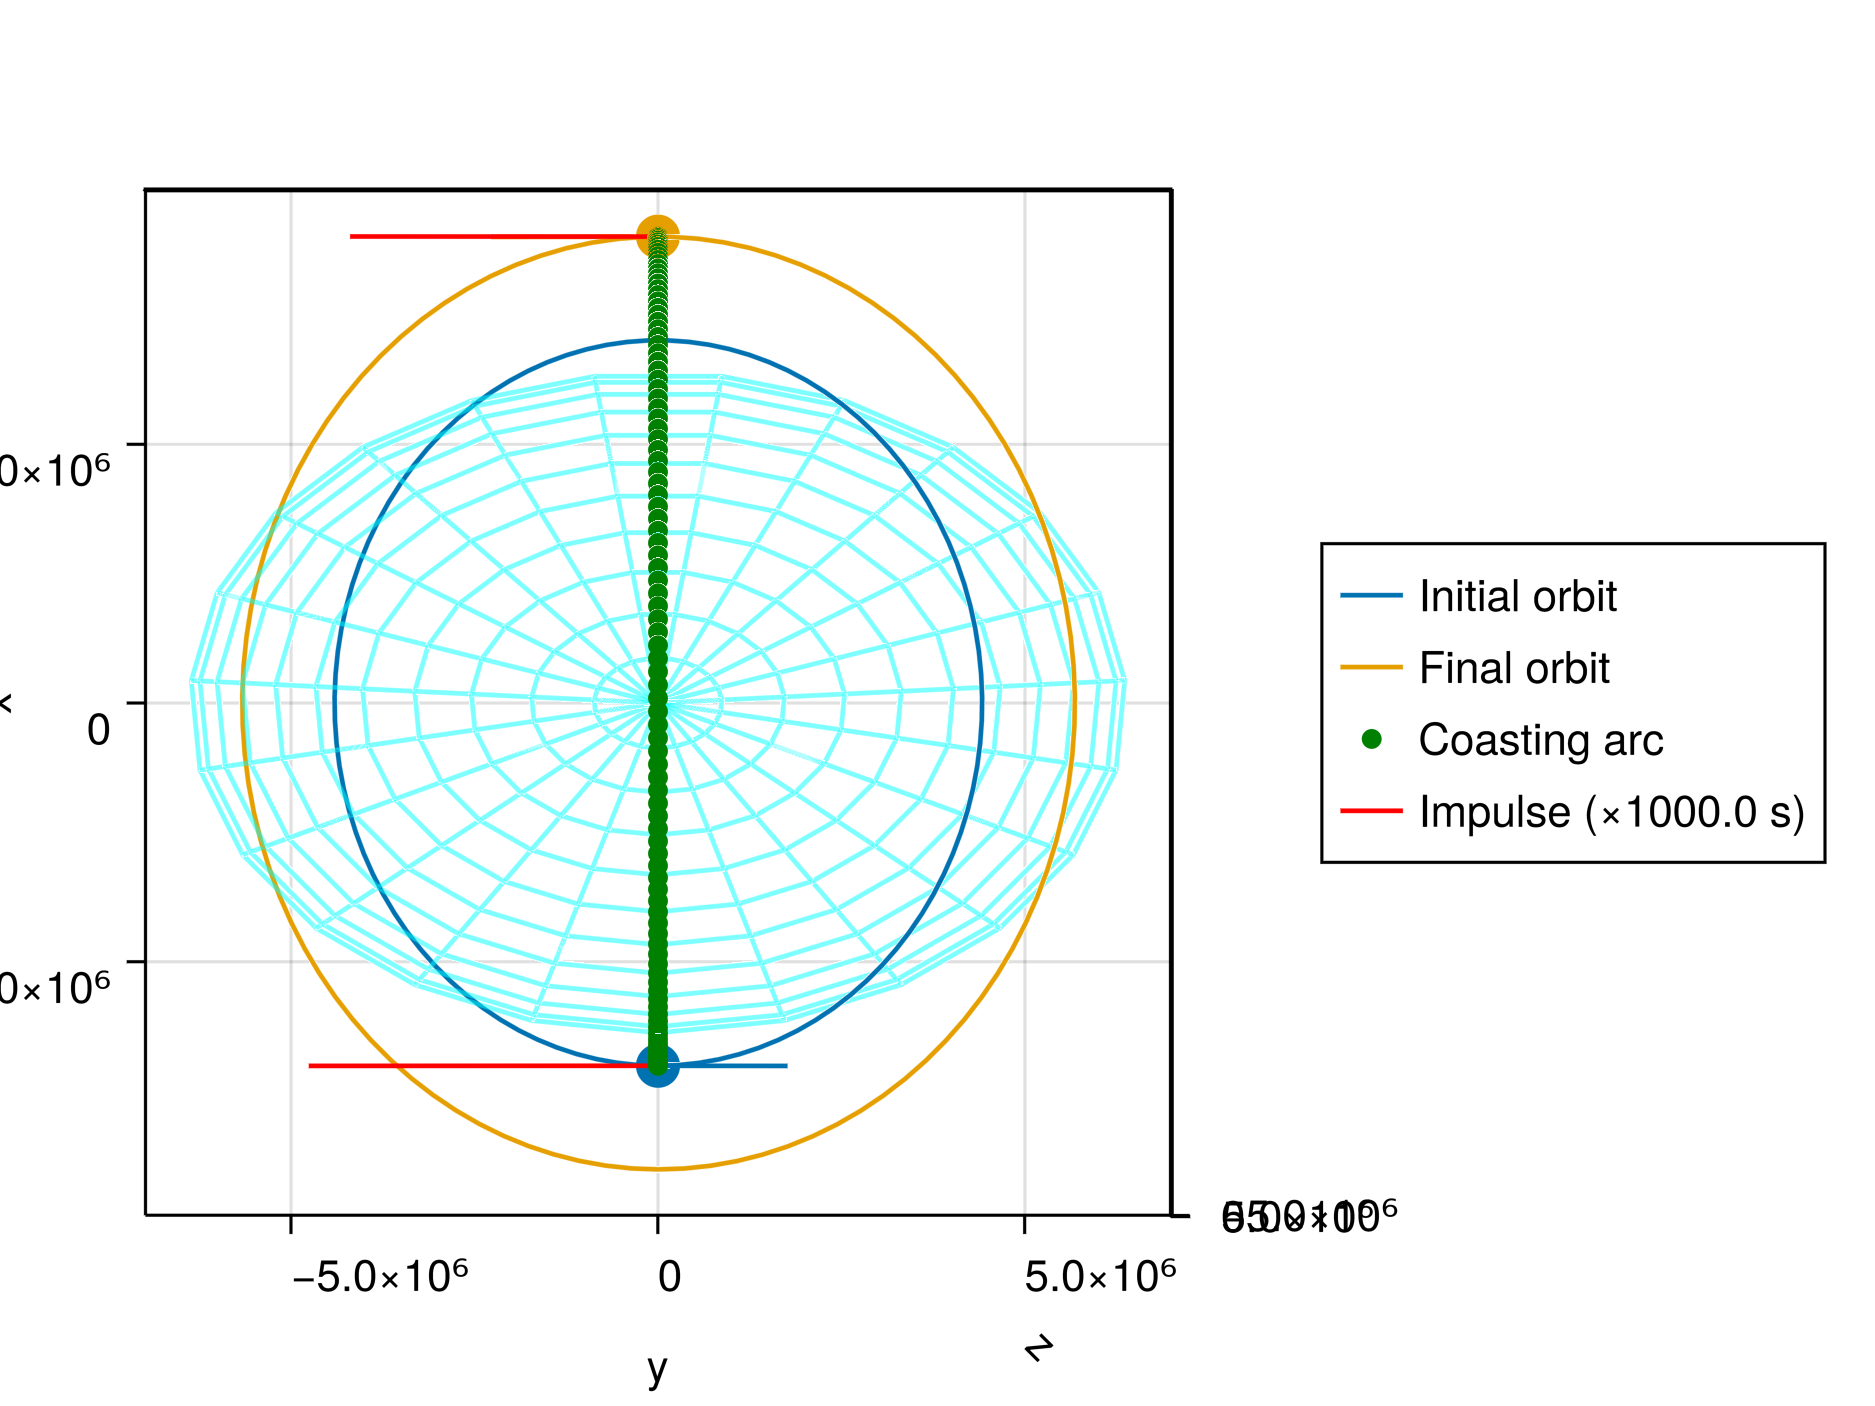
\includegraphics[width=\linewidth]{../results/j2/hohmann/ICI_z+.png}
        \caption{View from z+ axis.}
    \end{subfigure}
    \caption{Circle to circle \texttt{ICI} maneuver 3D view and projections}
    \label{fig:j2_c2c_ICI_figs}
\end{figure}

\begin{figure}[htbp]
    \centering
    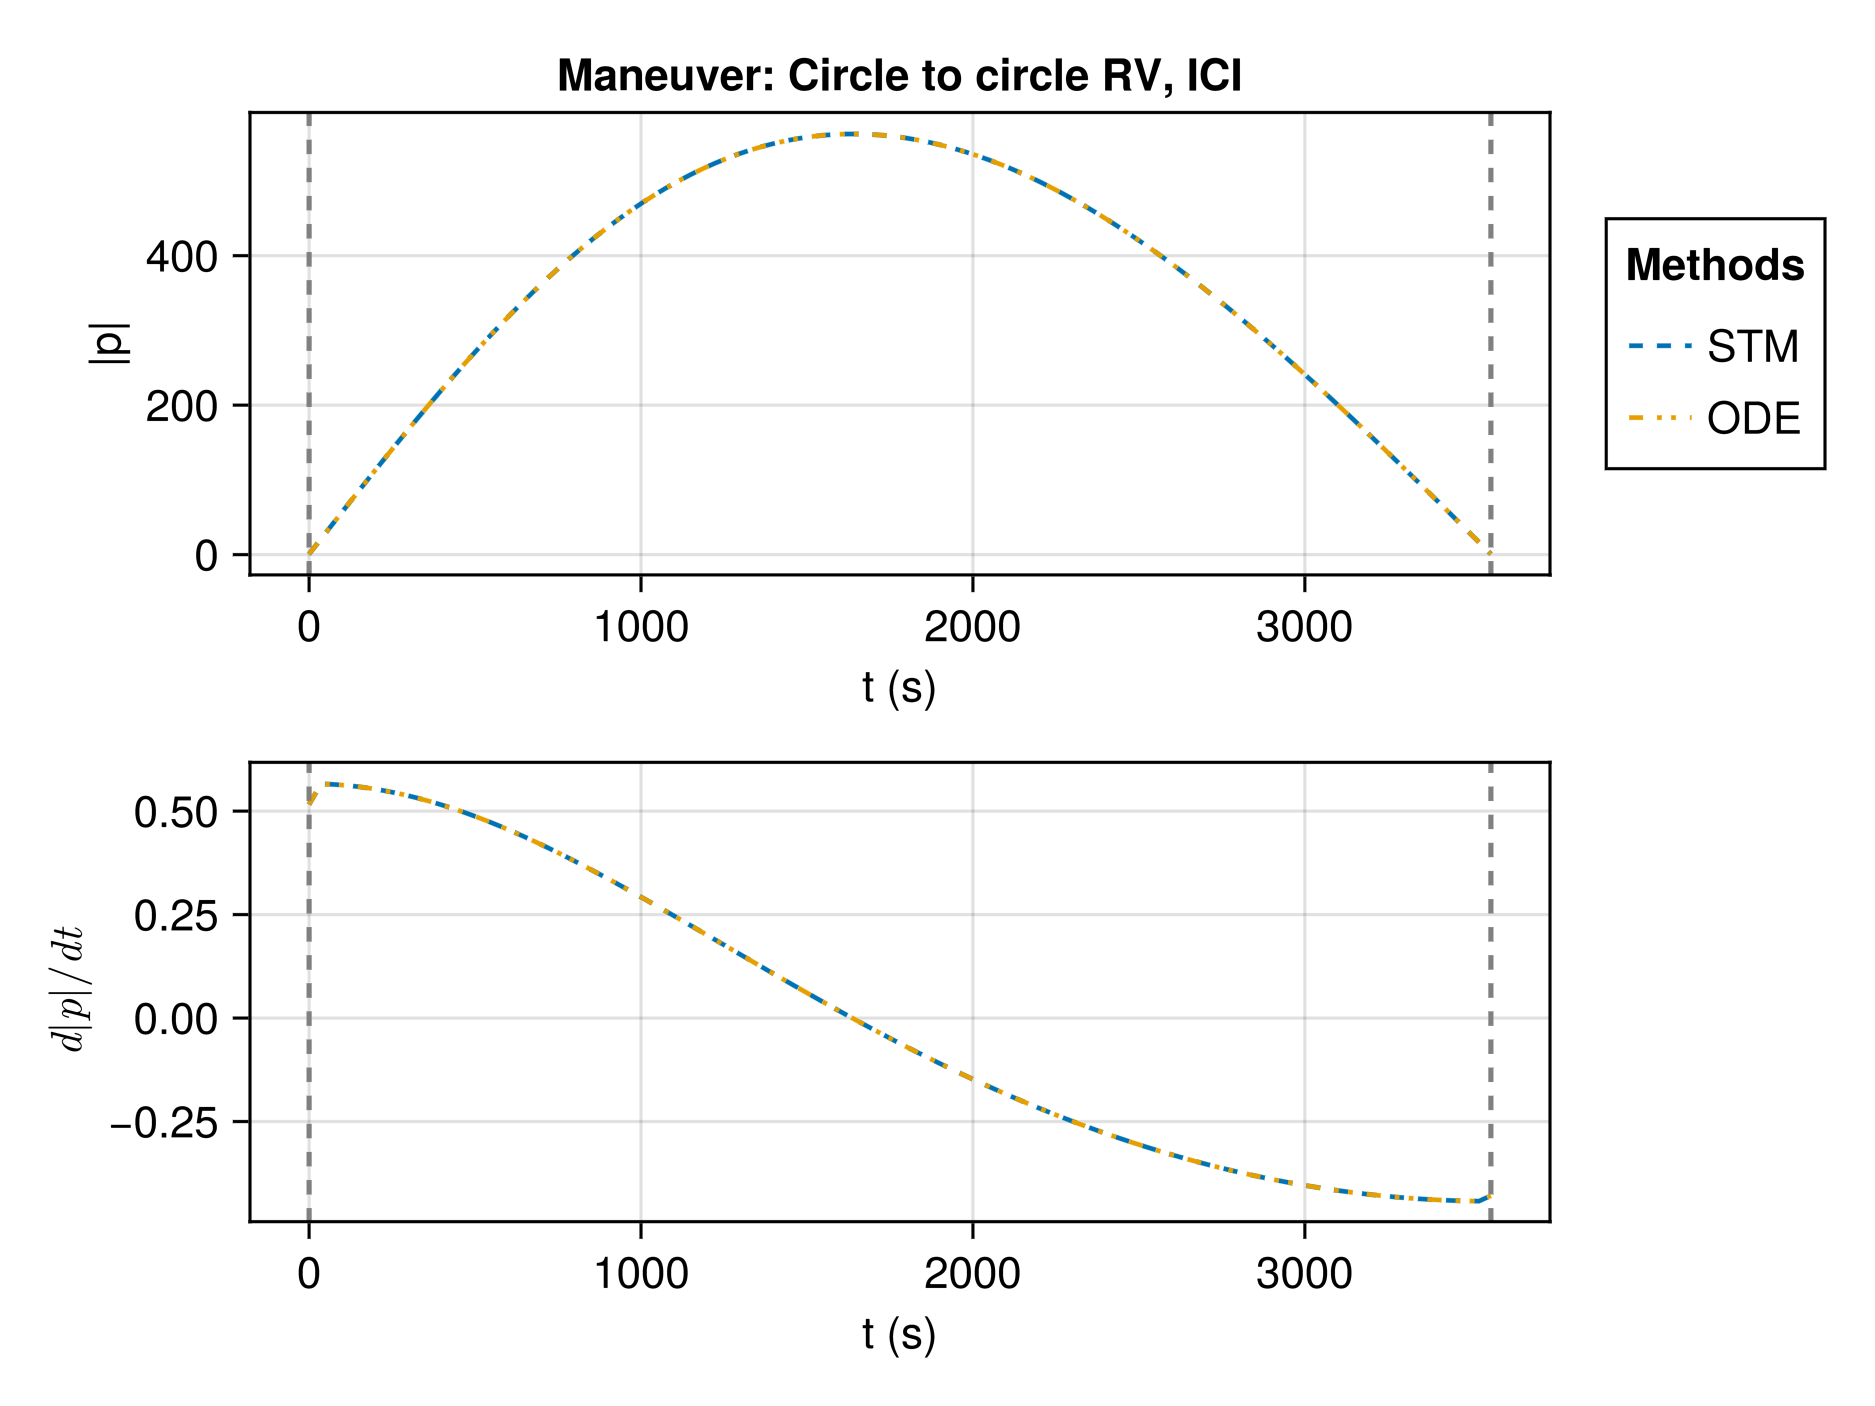
\includegraphics[width=\linewidth]{../results/j2/hohmann/ICI_primer_vector.png}
    \caption{Primer vector trajectory for J2 circle to circle \texttt{ICI} rendez-vous.}
    \label{fig:j2_c2c_ICI_pv}
\end{figure}

The solution of the \texttt{CICIC} maneuver is shown in Table~\ref{tab:j2_c2c_CICIC_tab}, Figure~\ref{fig:j2_c2c_CICIC_pv} and Figure~\ref{fig:j2_c2c_CICIC_figs}. The trajectory now closely resembles a Hohmann transfer, with the big difference that the impulses are not aligned with the velocities and that there are short initial and final coasts. Again, these differences can be explained mainly by the non-planarity of J2 coasting arcs. The primer vector trajectory indicates that this trajectory is not a local optimum in the \texttt{CICICIC} maneuver space, so adding another impulse should decrease the cost.

\begin{table}[htpb]
    \centering
    \begin{tabular}{cccc} \toprule
    \multicolumn{2}{c}{\textbf{Maneuver type}} & \multicolumn{2}{c}{CICIC} \\ \midrule
    \(L\) (m) & \(T\) (s) & \(\varepsilon\) & \(\Delta x_{f}\) (m)    \\ \midrule
    8.0e6          & 1.0          & 1.00e-05                & 4.0e-5                        \\ \midrule
    \(\max \lVert p \rVert\) & 2.0864     & \textbf{Diagnostic}   & Add impulse        \\ \midrule
    \textbf{Impulse} & \(t\) (s) & \(\Delta v\) (m/s) & \(1 - p \cdot \hat{u}\) \\ \midrule
    1                 & 72.53153          & 473.46697             & -0.0                    \\
    2                 & 3448.63865          & 438.46605             & -0.0                    \\\midrule
    \textbf{Total}   & 3560.54079          & 911.93302             &                     \\ \bottomrule   
    \end{tabular}
    \caption{Summary of optimization for J2 circle to circle \texttt{CICIC} rendez-vous.}
    \label{tab:j2_c2c_CICIC_tab}
\end{table}

\begin{figure}[htbp]
    \centering
    \begin{subfigure}{0.49\linewidth}
        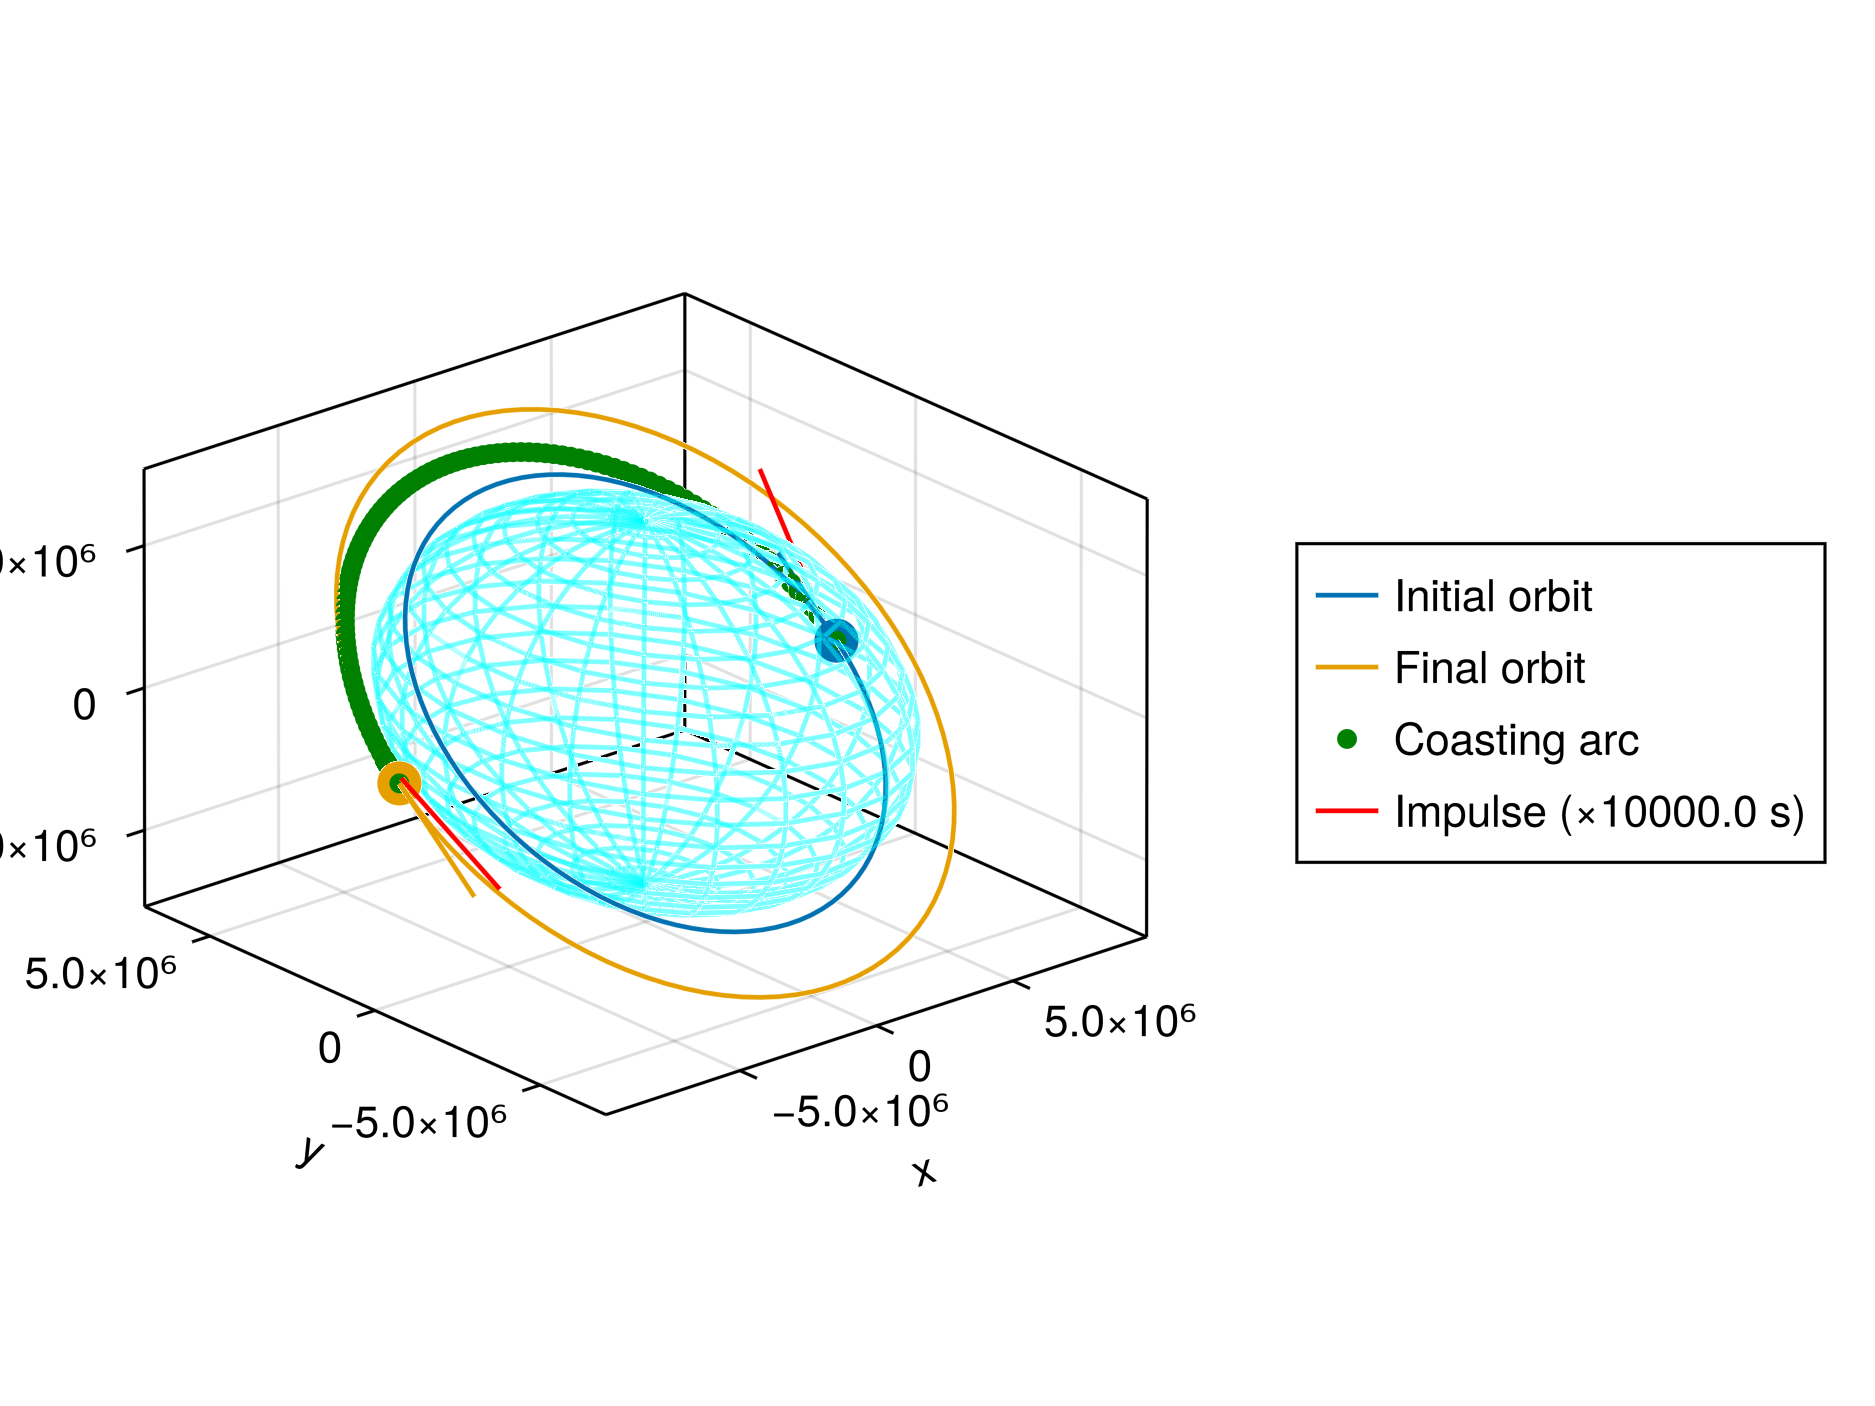
\includegraphics[width=\linewidth]{../results/j2/hohmann/CICIC_3d.png}
        \caption{3D view.}
    \end{subfigure}
    \begin{subfigure}{0.49\linewidth}
        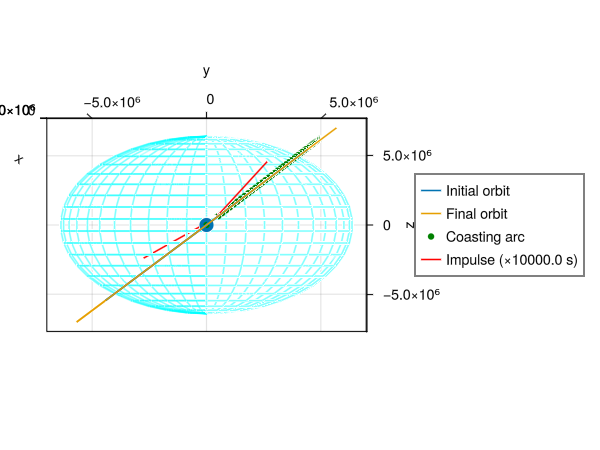
\includegraphics[width=\linewidth]{../results/j2/hohmann/CICIC_x+.png}
        \caption{View from x+ axis.}
    \end{subfigure}
    \begin{subfigure}{0.49\linewidth}
        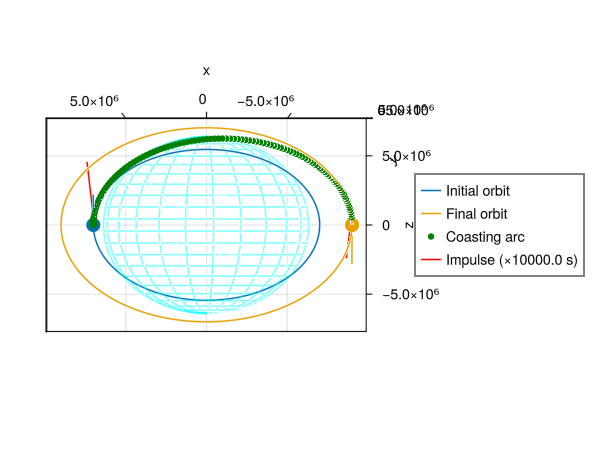
\includegraphics[width=\linewidth]{../results/j2/hohmann/CICIC_y+.png}
        \caption{View from y+ axis.}
    \end{subfigure}
    \begin{subfigure}{0.49\linewidth}
        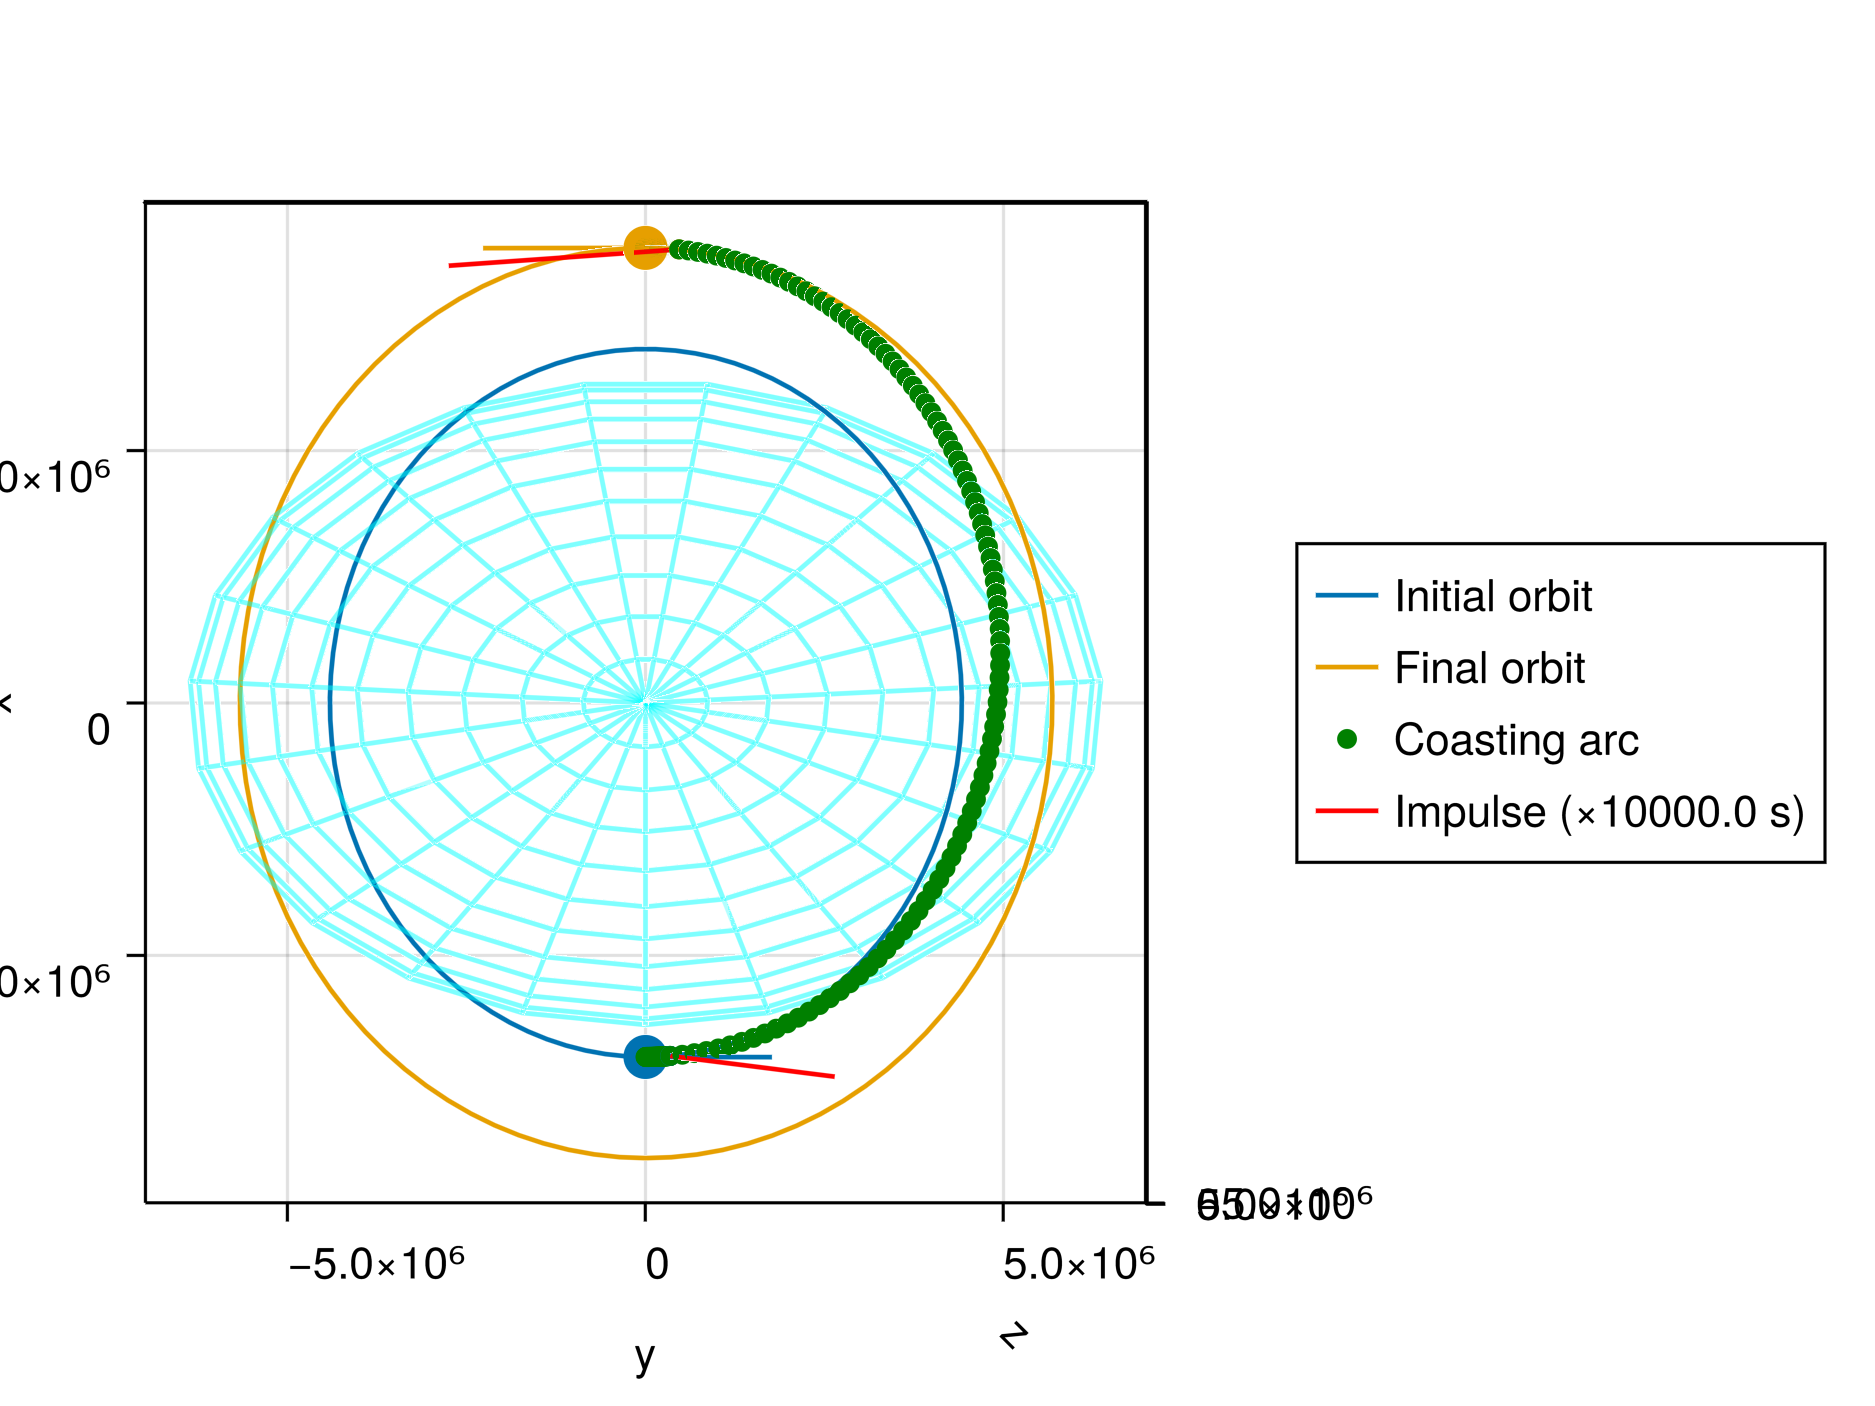
\includegraphics[width=\linewidth]{../results/j2/hohmann/CICIC_z+.png}
        \caption{View from z+ axis.}
    \end{subfigure}
    \caption{Circle to circle \texttt{CICIC} maneuver 3D view and projections}
    \label{fig:j2_c2c_CICIC_figs}
\end{figure}

\begin{figure}[htbp]
    \centering
    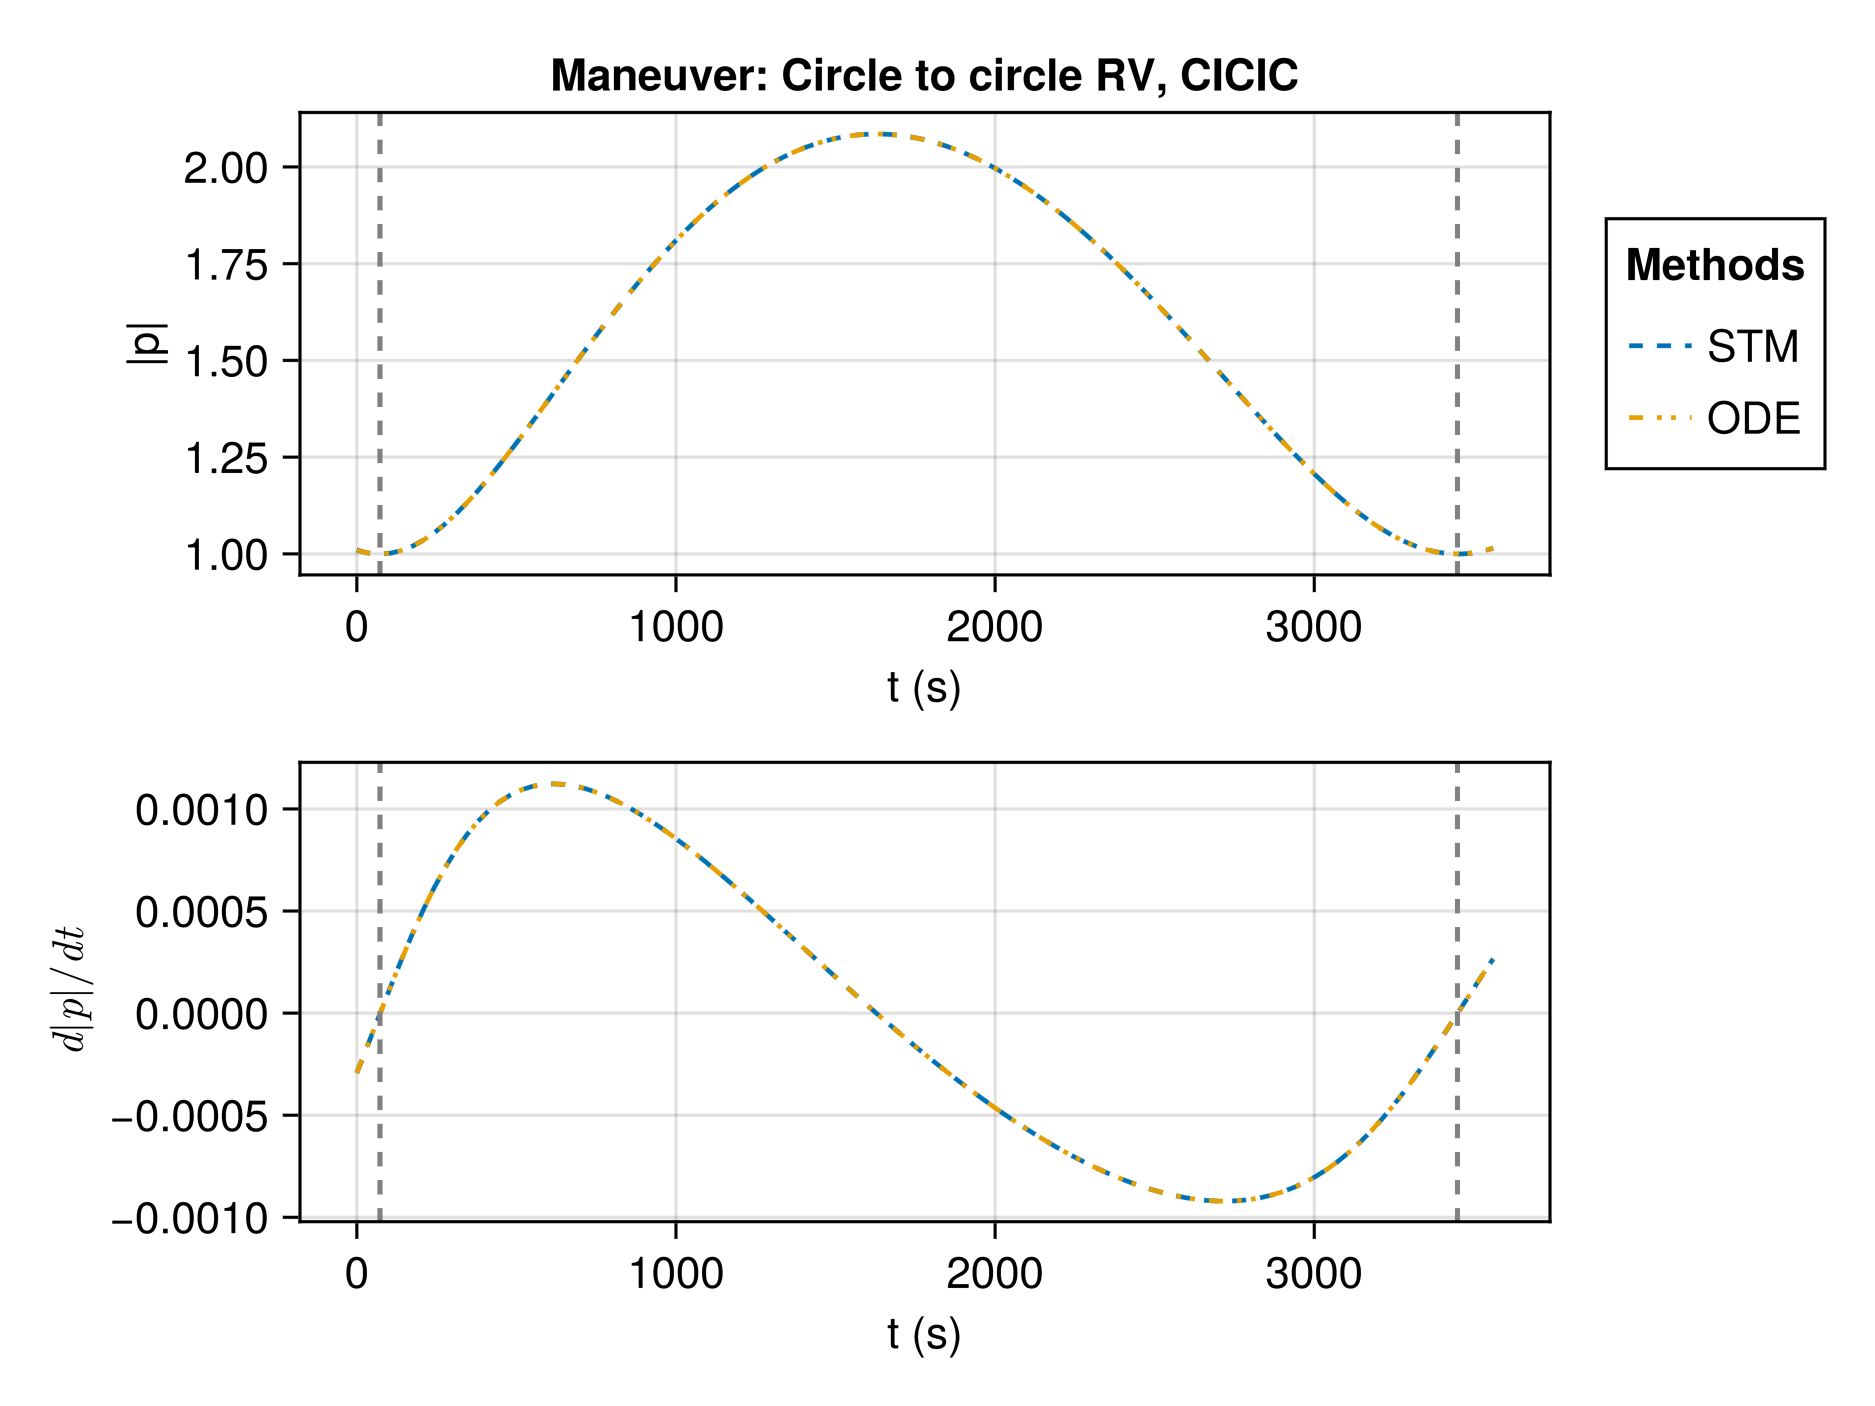
\includegraphics[width=\linewidth]{../results/j2/hohmann/CICIC_primer_vector.png}
    \caption{Primer vector trajectory for two body circle to circle \texttt{CICIC} rendez-vous.}
    \label{fig:j2_c2c_CICIC_pv}
\end{figure}

Now, the \texttt{CICICIC} case is solved, with a summary shown in Table~\ref{tab:j2_c2c_CICICIC_tab}, primer vector trajectory shown in Figure~\ref{fig:j2_c2c_CICICIC_pv}, and spatial views in Figure~\ref{fig:j2_c2c_CICICIC_figs}. Now, two large impulses are made close to the endpoints, and a very small intermediate impulse is made about halfway throught the maneuver. The necessary conditions for optimality are satisfied with 3 impulses, and the final cost of the J2 model is about \(6 m/s\) higher than under the two body model.


\begin{table}[htpb]
    \centering
    \begin{tabular}{cccc} \toprule
    \multicolumn{2}{c}{\textbf{Maneuver type}} & \multicolumn{2}{c}{CICICIC} \\ \midrule
    \(L\) (m) & \(T\) (s) & \(\varepsilon\) & \(\Delta x_{f}\) (m)    \\ \midrule
    8.0e6          & 1.0          & 1.00e-05                & 0.02201                        \\ \midrule
    \(\max \lVert p \rVert\) & 1.0     & \textbf{Diagnostic}   & Local optimum        \\ \midrule
    \textbf{Impulse} & \(t\) (s) & \(\Delta v\) (m/s) & \(1 - p \cdot \hat{u}\) \\ \midrule
    1                 & 0.38763          & 451.26267             & -0.0                    \\
    2                 & 1697.05494          & 25.16996             & -0.0                    \\
    3                 & 3559.91404          & 416.62074             & -0.0                    \\\midrule
    \textbf{Total}   & 3560.54079          & 893.05336             &                     \\ \bottomrule   
    \end{tabular}
    \caption{Summary of optimization for J2 circle to circle \texttt{CICICIC} rendez-vous.}
    \label{tab:j2_c2c_CICICIC_tab}
\end{table}

\begin{figure}[htbp]
    \centering
    \begin{subfigure}{0.49\linewidth}
        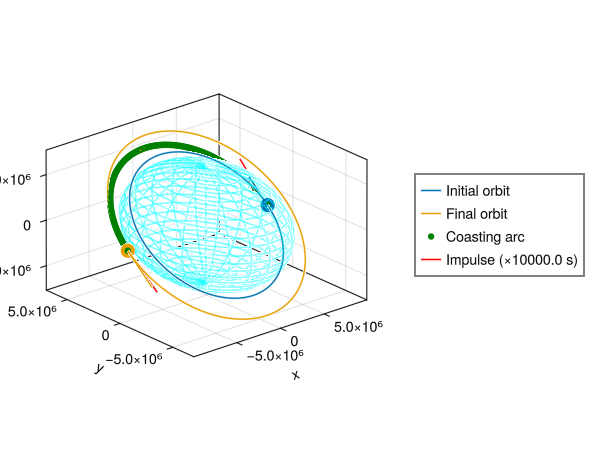
\includegraphics[width=\linewidth]{../results/j2/hohmann/CICICIC_3d.png}
        \caption{3D view.}
    \end{subfigure}
    \begin{subfigure}{0.49\linewidth}
        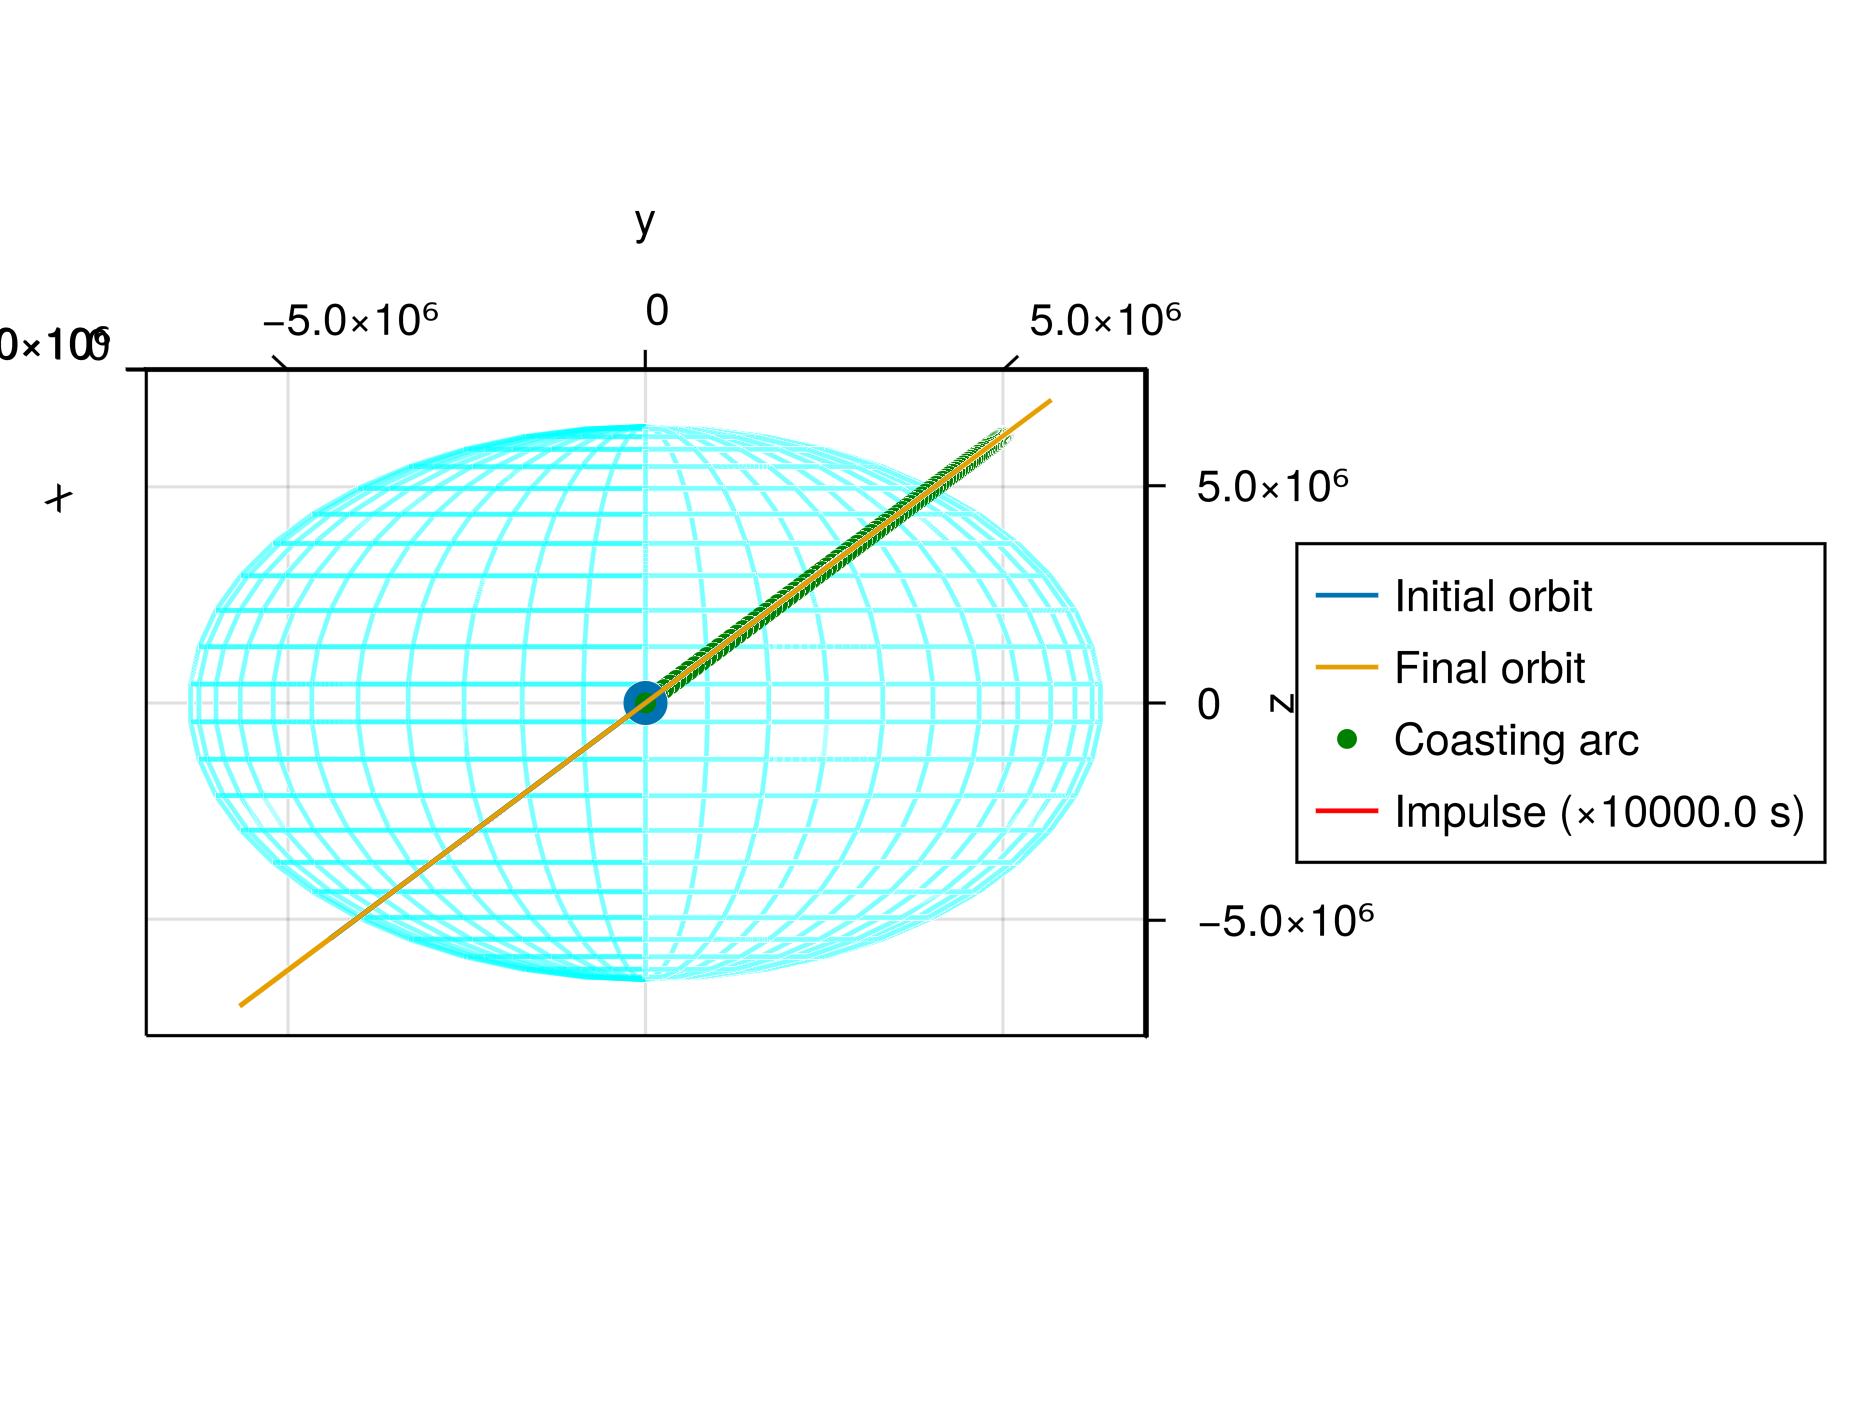
\includegraphics[width=\linewidth]{../results/j2/hohmann/CICICIC_x+.png}
        \caption{View from x+ axis.}
    \end{subfigure}
    \begin{subfigure}{0.49\linewidth}
        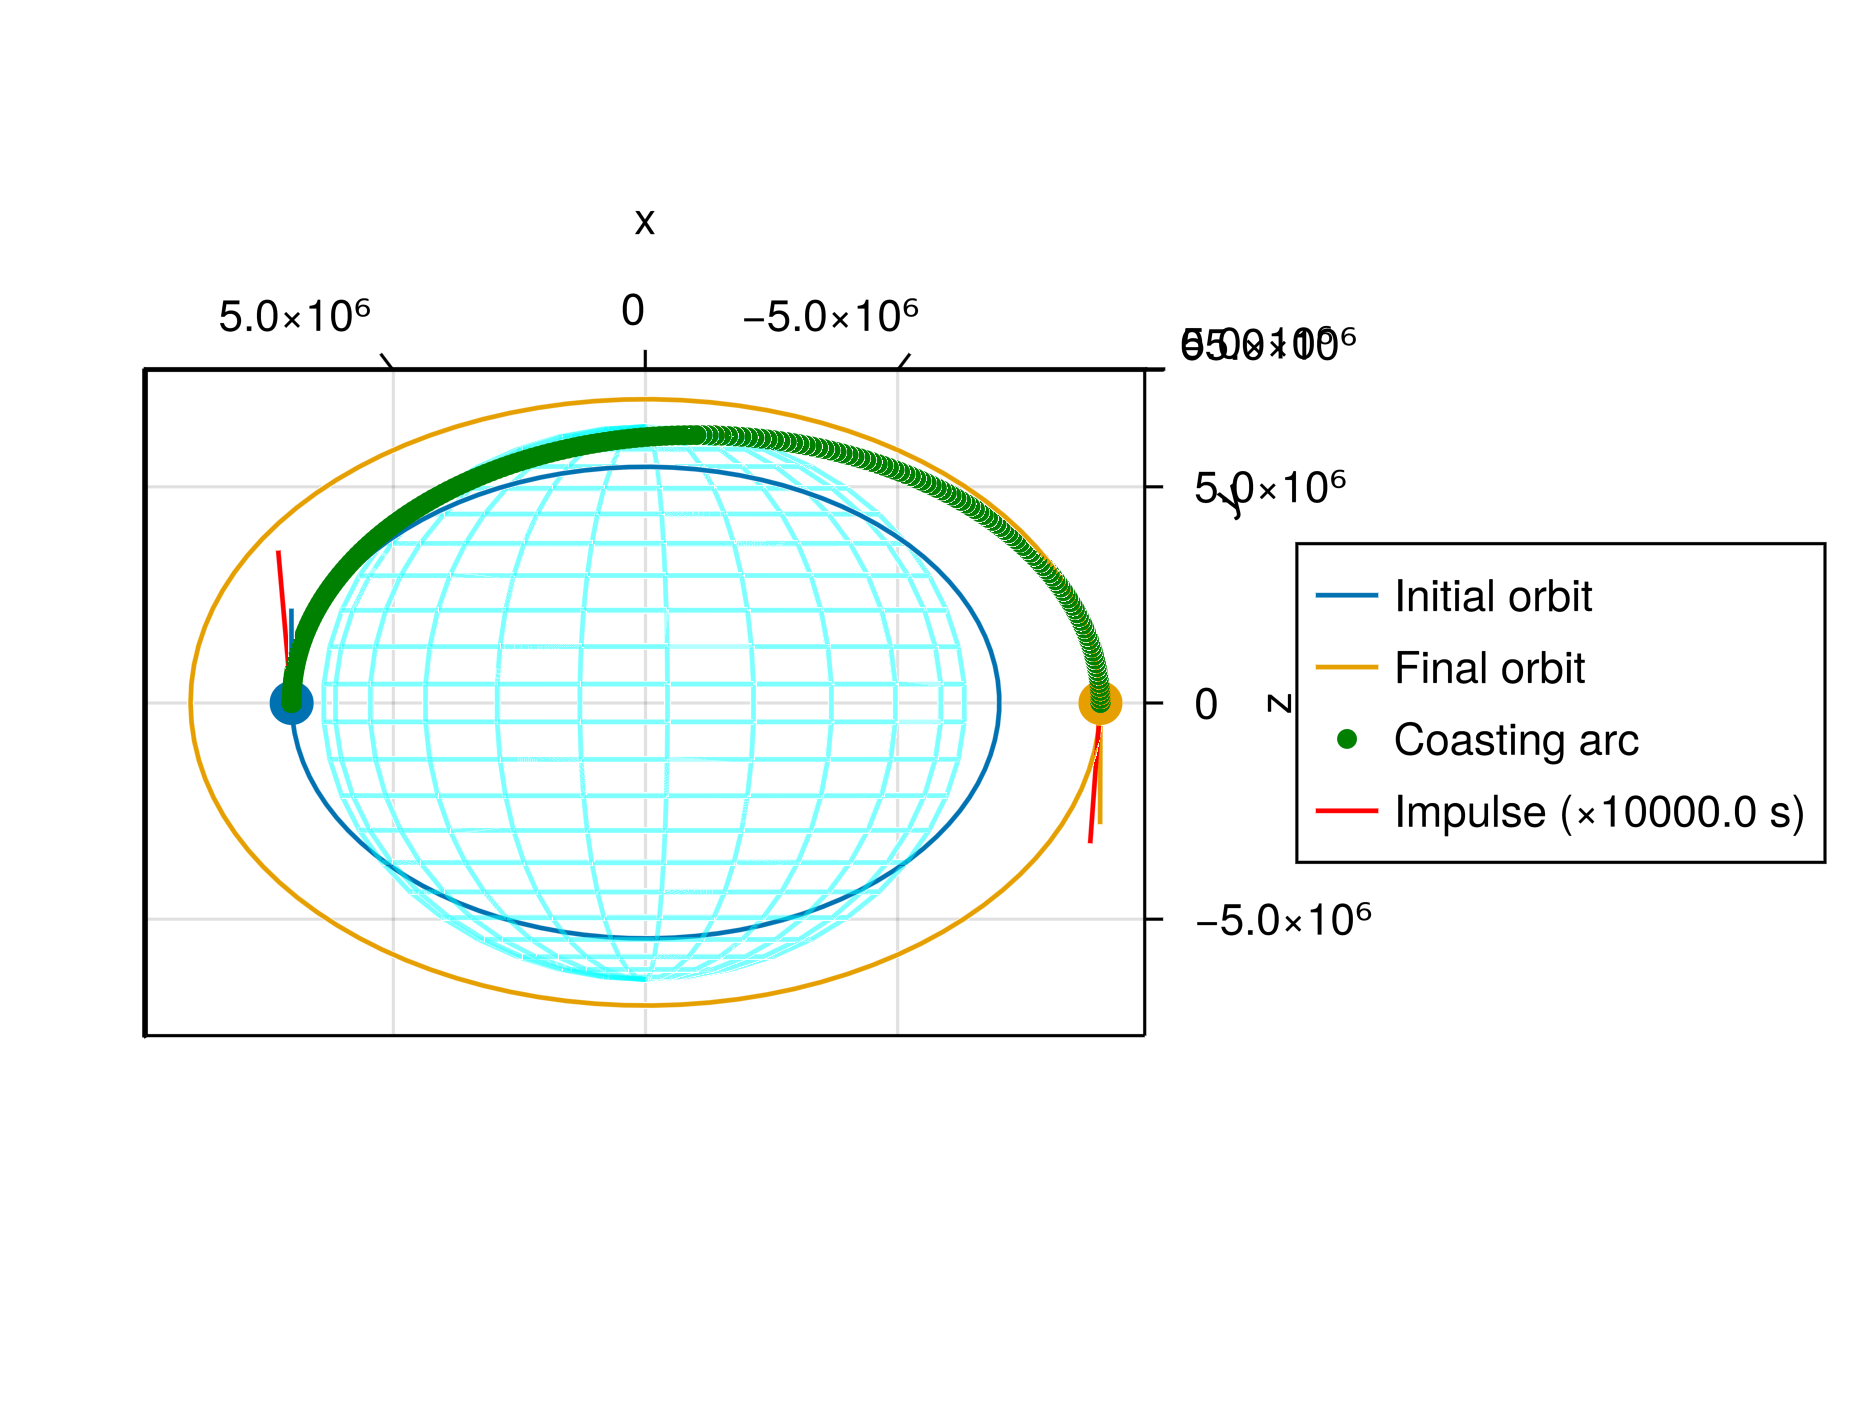
\includegraphics[width=\linewidth]{../results/j2/hohmann/CICICIC_y+.png}
        \caption{View from y+ axis.}
    \end{subfigure}
    \begin{subfigure}{0.49\linewidth}
        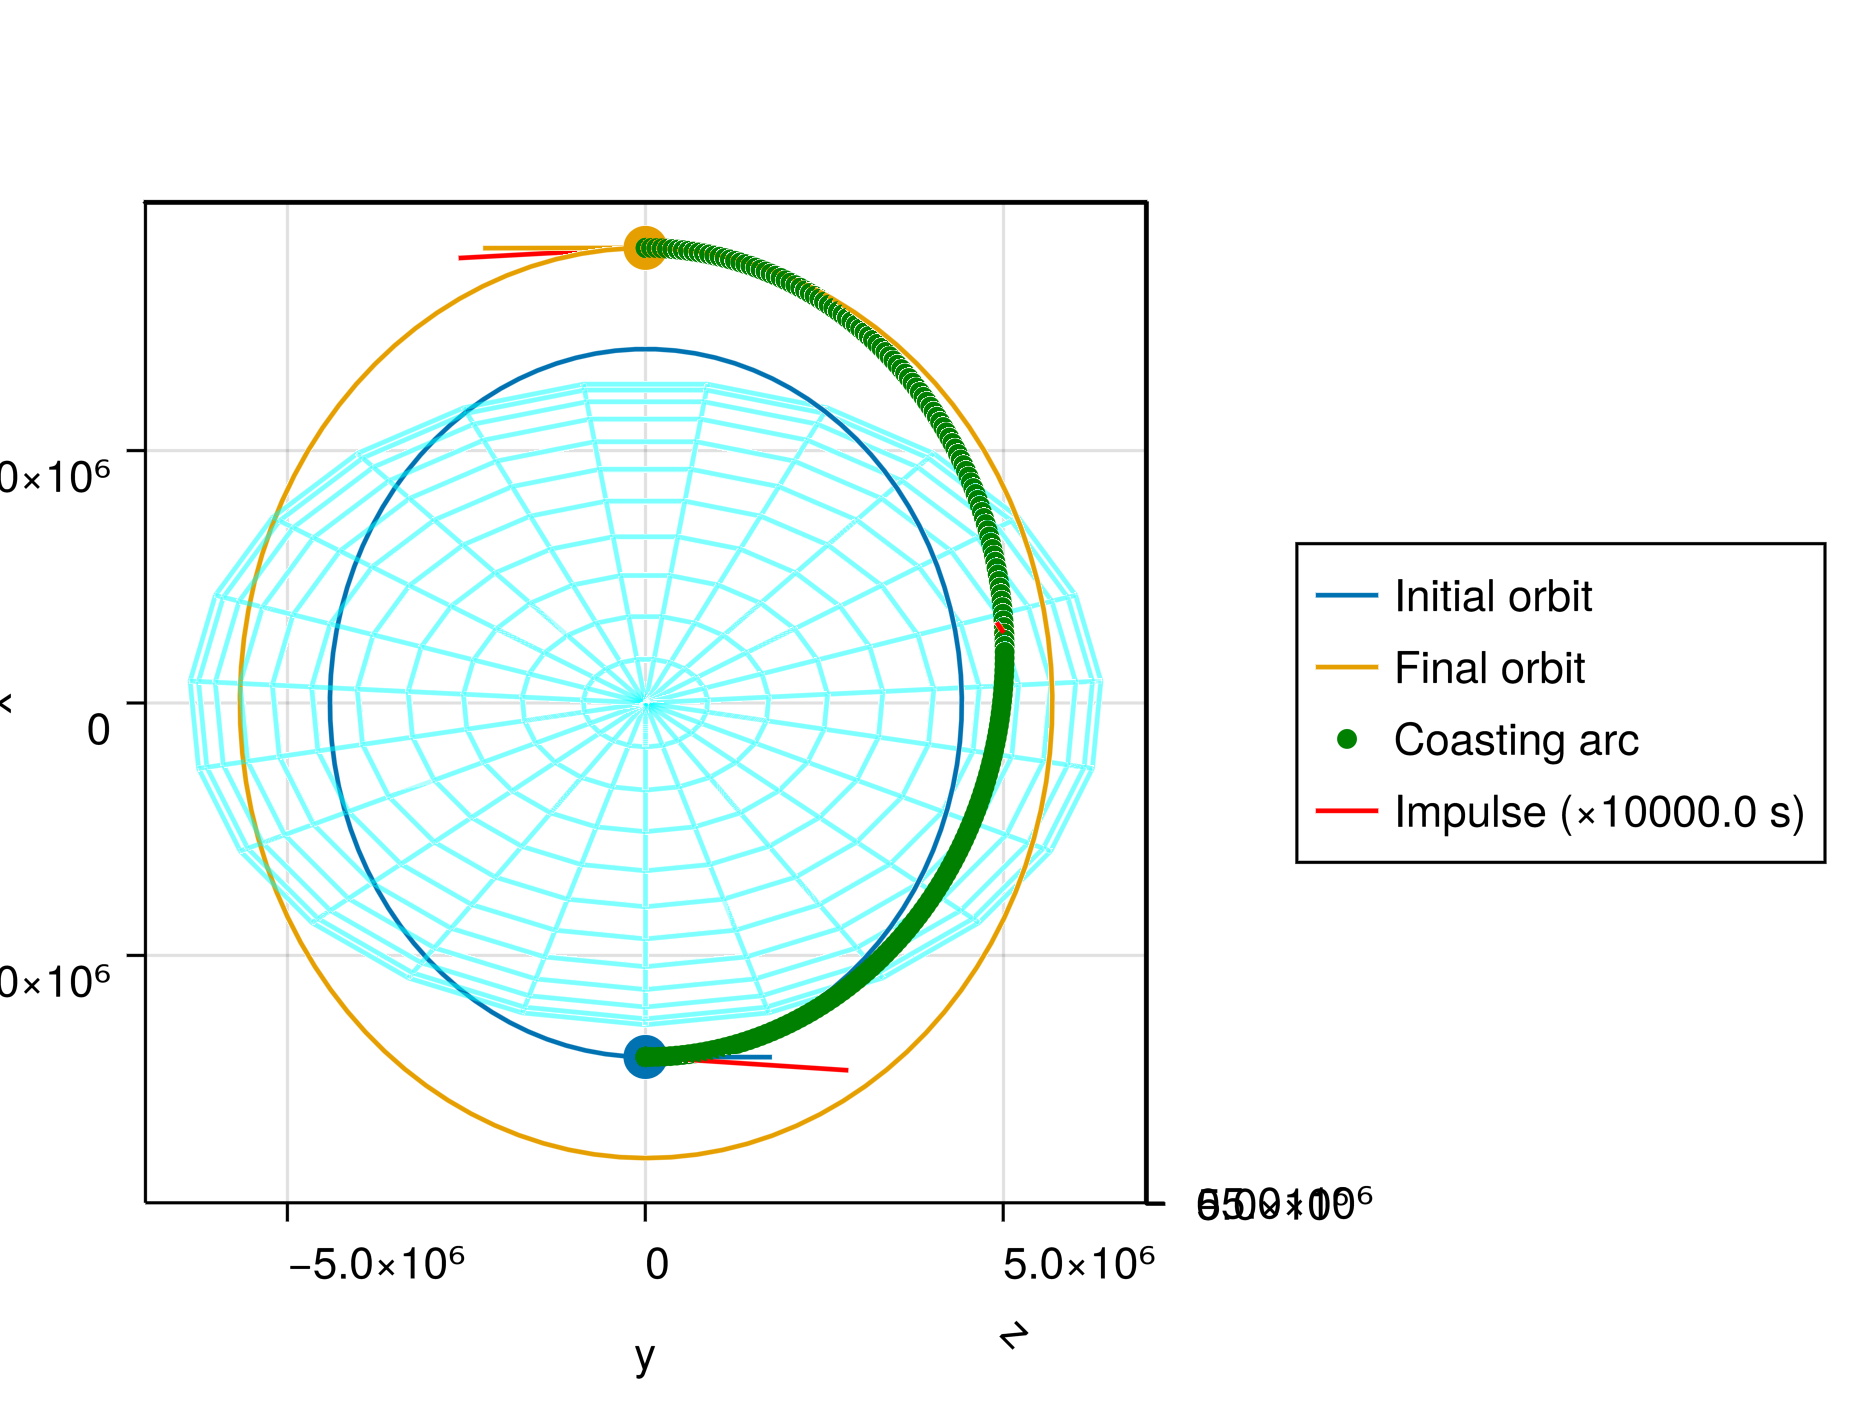
\includegraphics[width=\linewidth]{../results/j2/hohmann/CICICIC_z+.png}
        \caption{View from z+ axis.}
    \end{subfigure}
    \caption{Circle to circle \texttt{CICICIC} maneuver 3D view and projections}
    \label{fig:j2_c2c_CICICIC_figs}
\end{figure}

\begin{figure}[htbp]
    \centering
    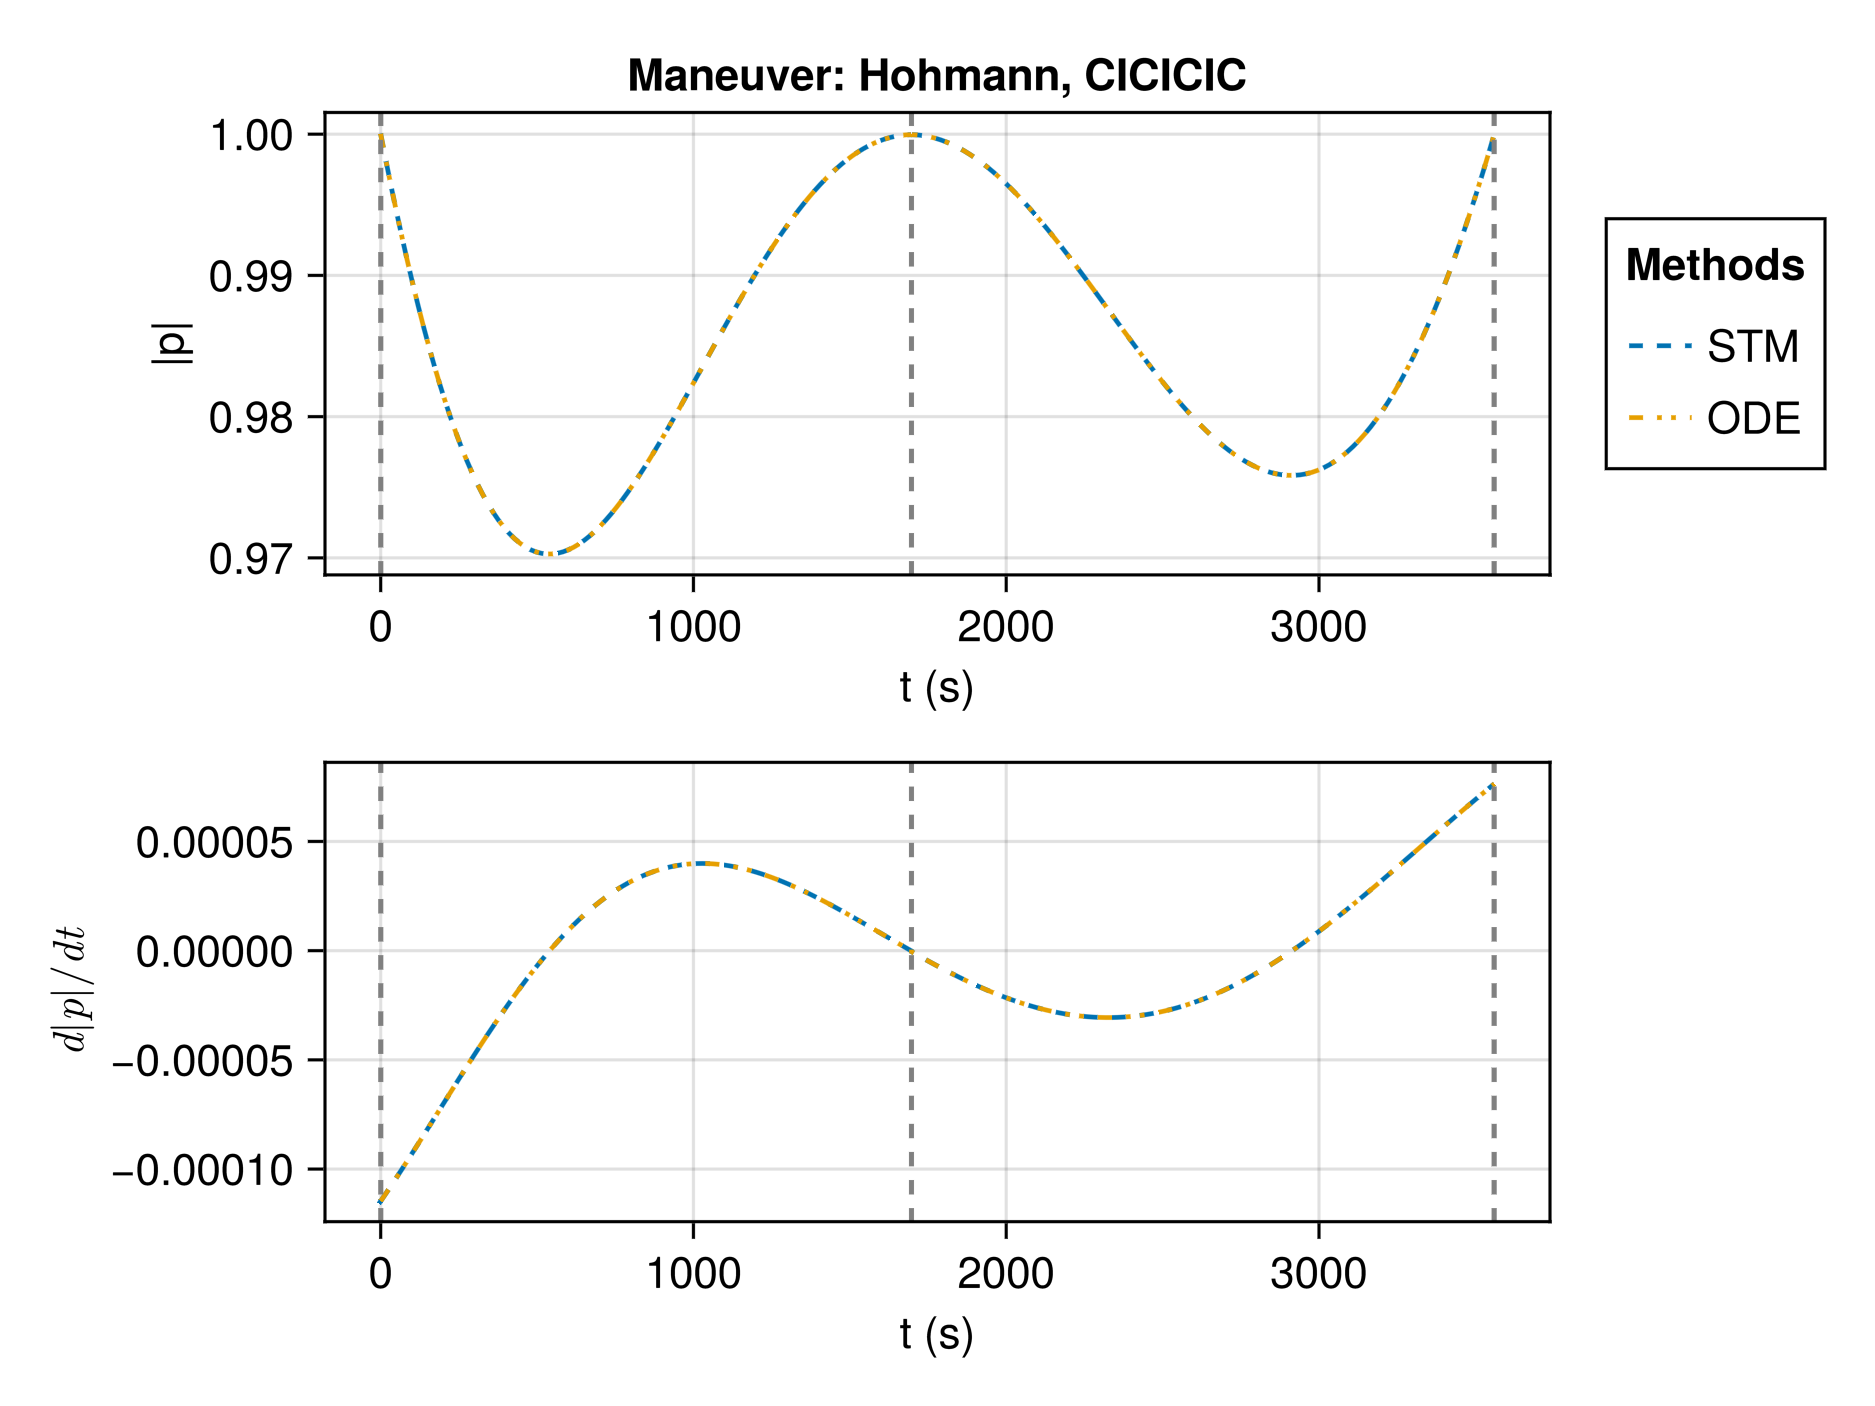
\includegraphics[width=\linewidth]{../results/j2/hohmann/CICICIC_primer_vector.png}
    \caption{Primer vector trajectory for two body circle to circle \texttt{CICICIC} rendez-vous.}
    \label{fig:j2_c2c_CICICIC_pv}
\end{figure}

\subsection{Noncoplanar rendez-vous}

Now, the noncoplanar rendez-vous scenario is tackled under the J2 model. As usual, the first maneuver to be solved was a \texttt{ICI} case. The maneuver summary is given in Table~\ref{tab:j2_ncop_ICI_tab}, the primer vector trajectory in Figure~\ref{fig:j2_ncop_ICI_pv}, and spatial views in Figure~\ref{fig:j2_ncop_ICI_figs}. Under this model, the non-planarity of the J2 orbits allow for a feasible \texttt{ICI} maneuver with multiple revolutions, much cheaper than the equivalent two-body maneuver. The maneuver does not satisfy primer vector necessary conditions, including the continuity of the primer vector derivative. Primer vector analysis recommends adding initial and final coasts.

\begin{table}[htpb]
    \centering
    \begin{tabular}{cccc} \toprule
    \multicolumn{2}{c}{\textbf{Maneuver type}} & \multicolumn{2}{c}{ICI} \\ \midrule
    \(L\) (m) & \(T\) (s) & \(\varepsilon\) & \(\Delta x_{f}\) (m)    \\ \midrule
    6.7631e6          & 11107.158          & 1.00e-05                & 3.63678                        \\ \midrule
    \(\max \lVert p \rVert\) & 65.441     & \textbf{Diagnostic}   & Initial + final coast        \\ \midrule
    \textbf{Impulse} & \(t\) (s) & \(\Delta v\) (m/s) & \(1 - p \cdot \hat{u}\) \\ \midrule
    1                 & 0.0          & 743.66668             & -0.0                    \\
    2                 & 11107.1576          & 727.80415             & -0.0                    \\\midrule
    \textbf{Total}   & 11107.1576          & 1471.47082             &                     \\ \bottomrule   
    \end{tabular}
    \caption{Summary of optimization for J2 noncoplanar \texttt{ICI} rendez-vous.}
    \label{tab:j2_ncop_ICI_tab}
\end{table}

\begin{figure}[htbp]
    \centering
    \begin{subfigure}{0.49\linewidth}
        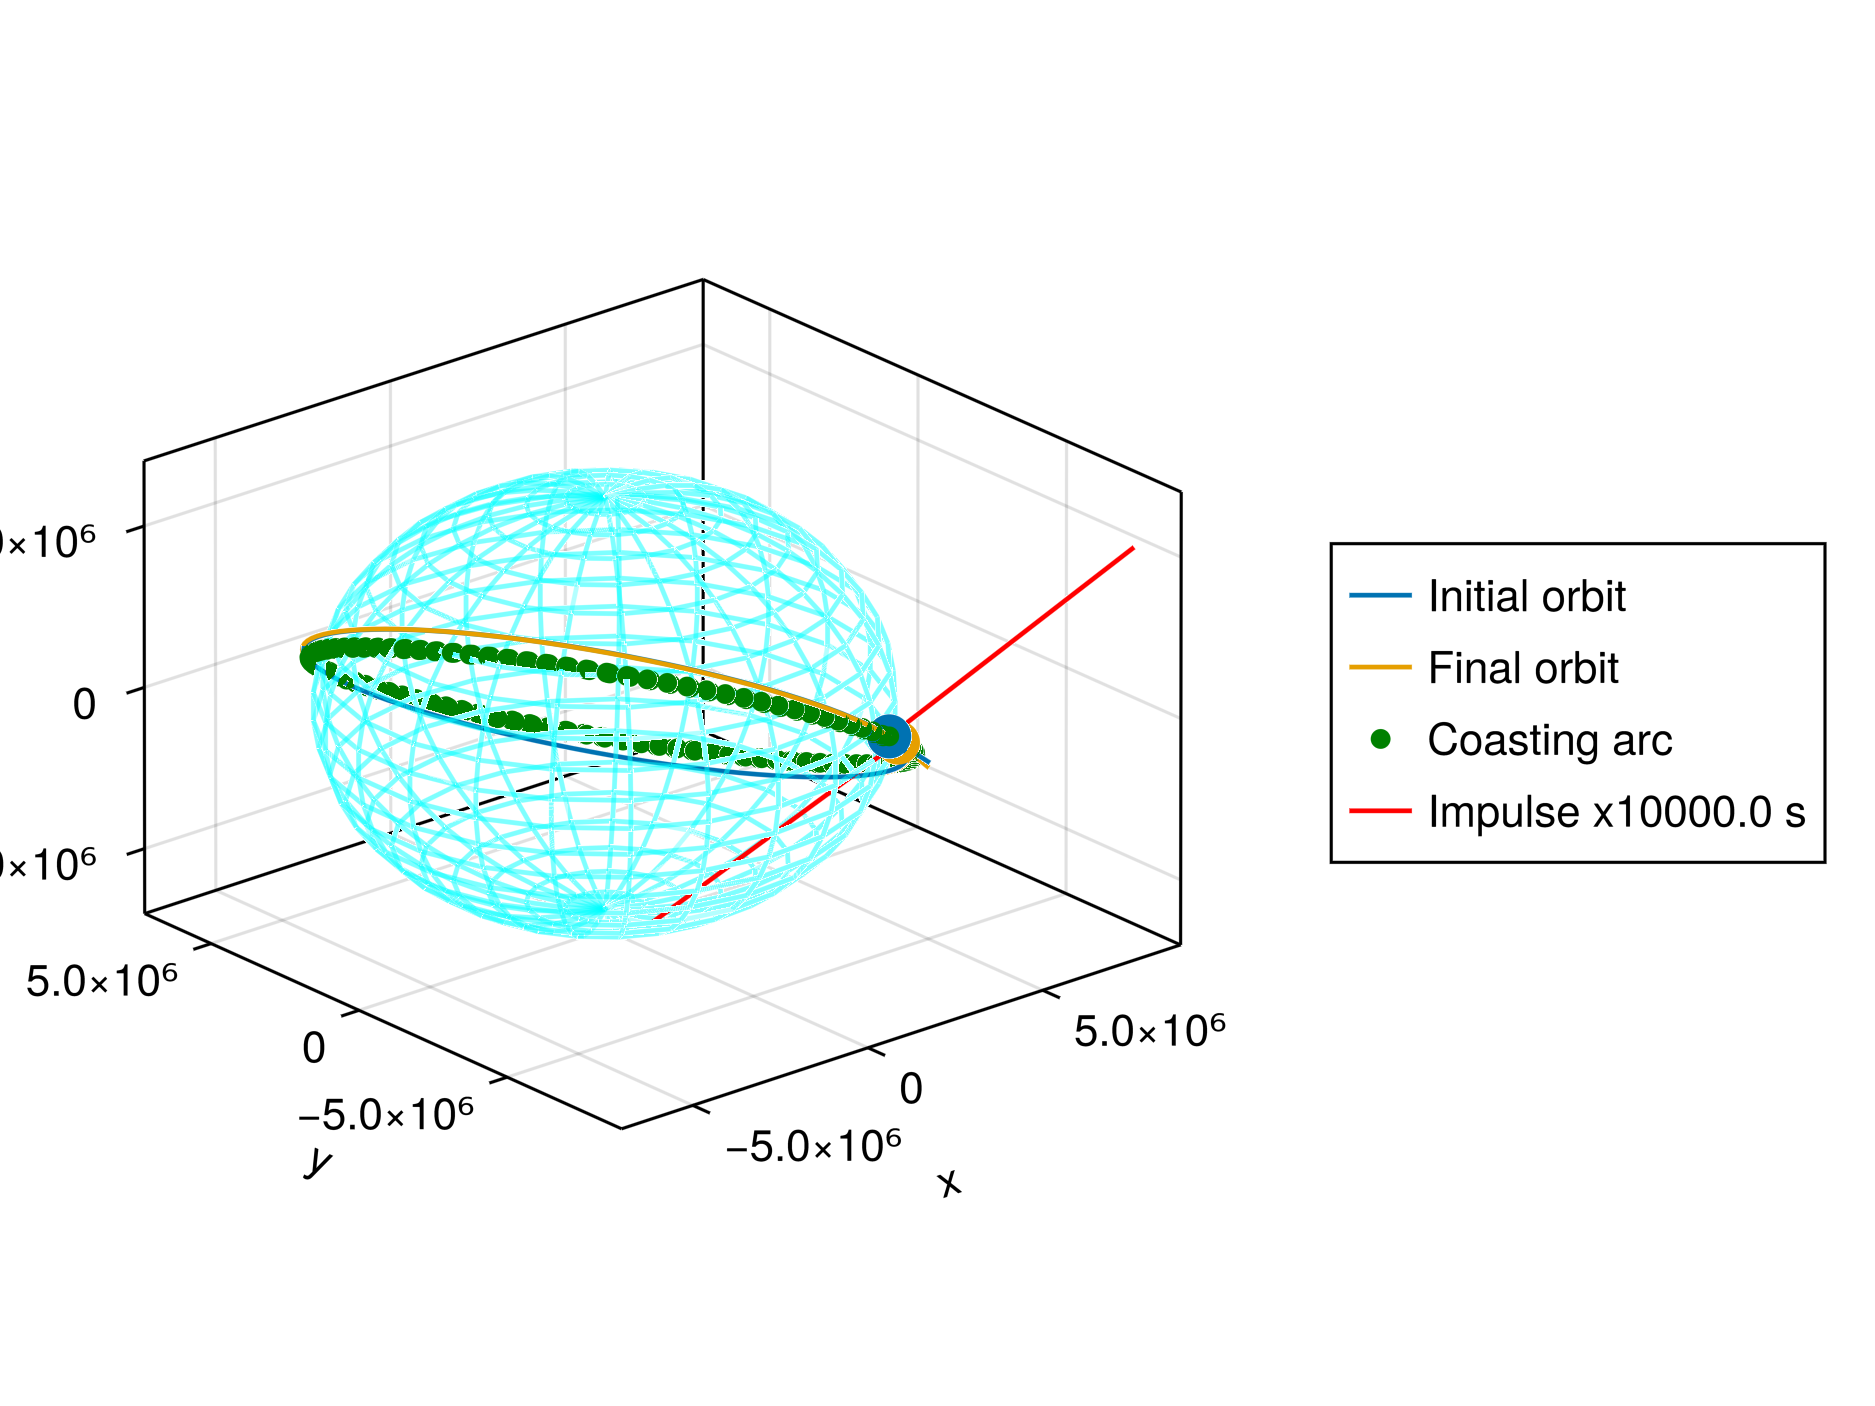
\includegraphics[width=\linewidth]{../results/j2/ipv_noncop/ICI_3d.png}
        \caption{3D view.}
    \end{subfigure}
    \begin{subfigure}{0.49\linewidth}
        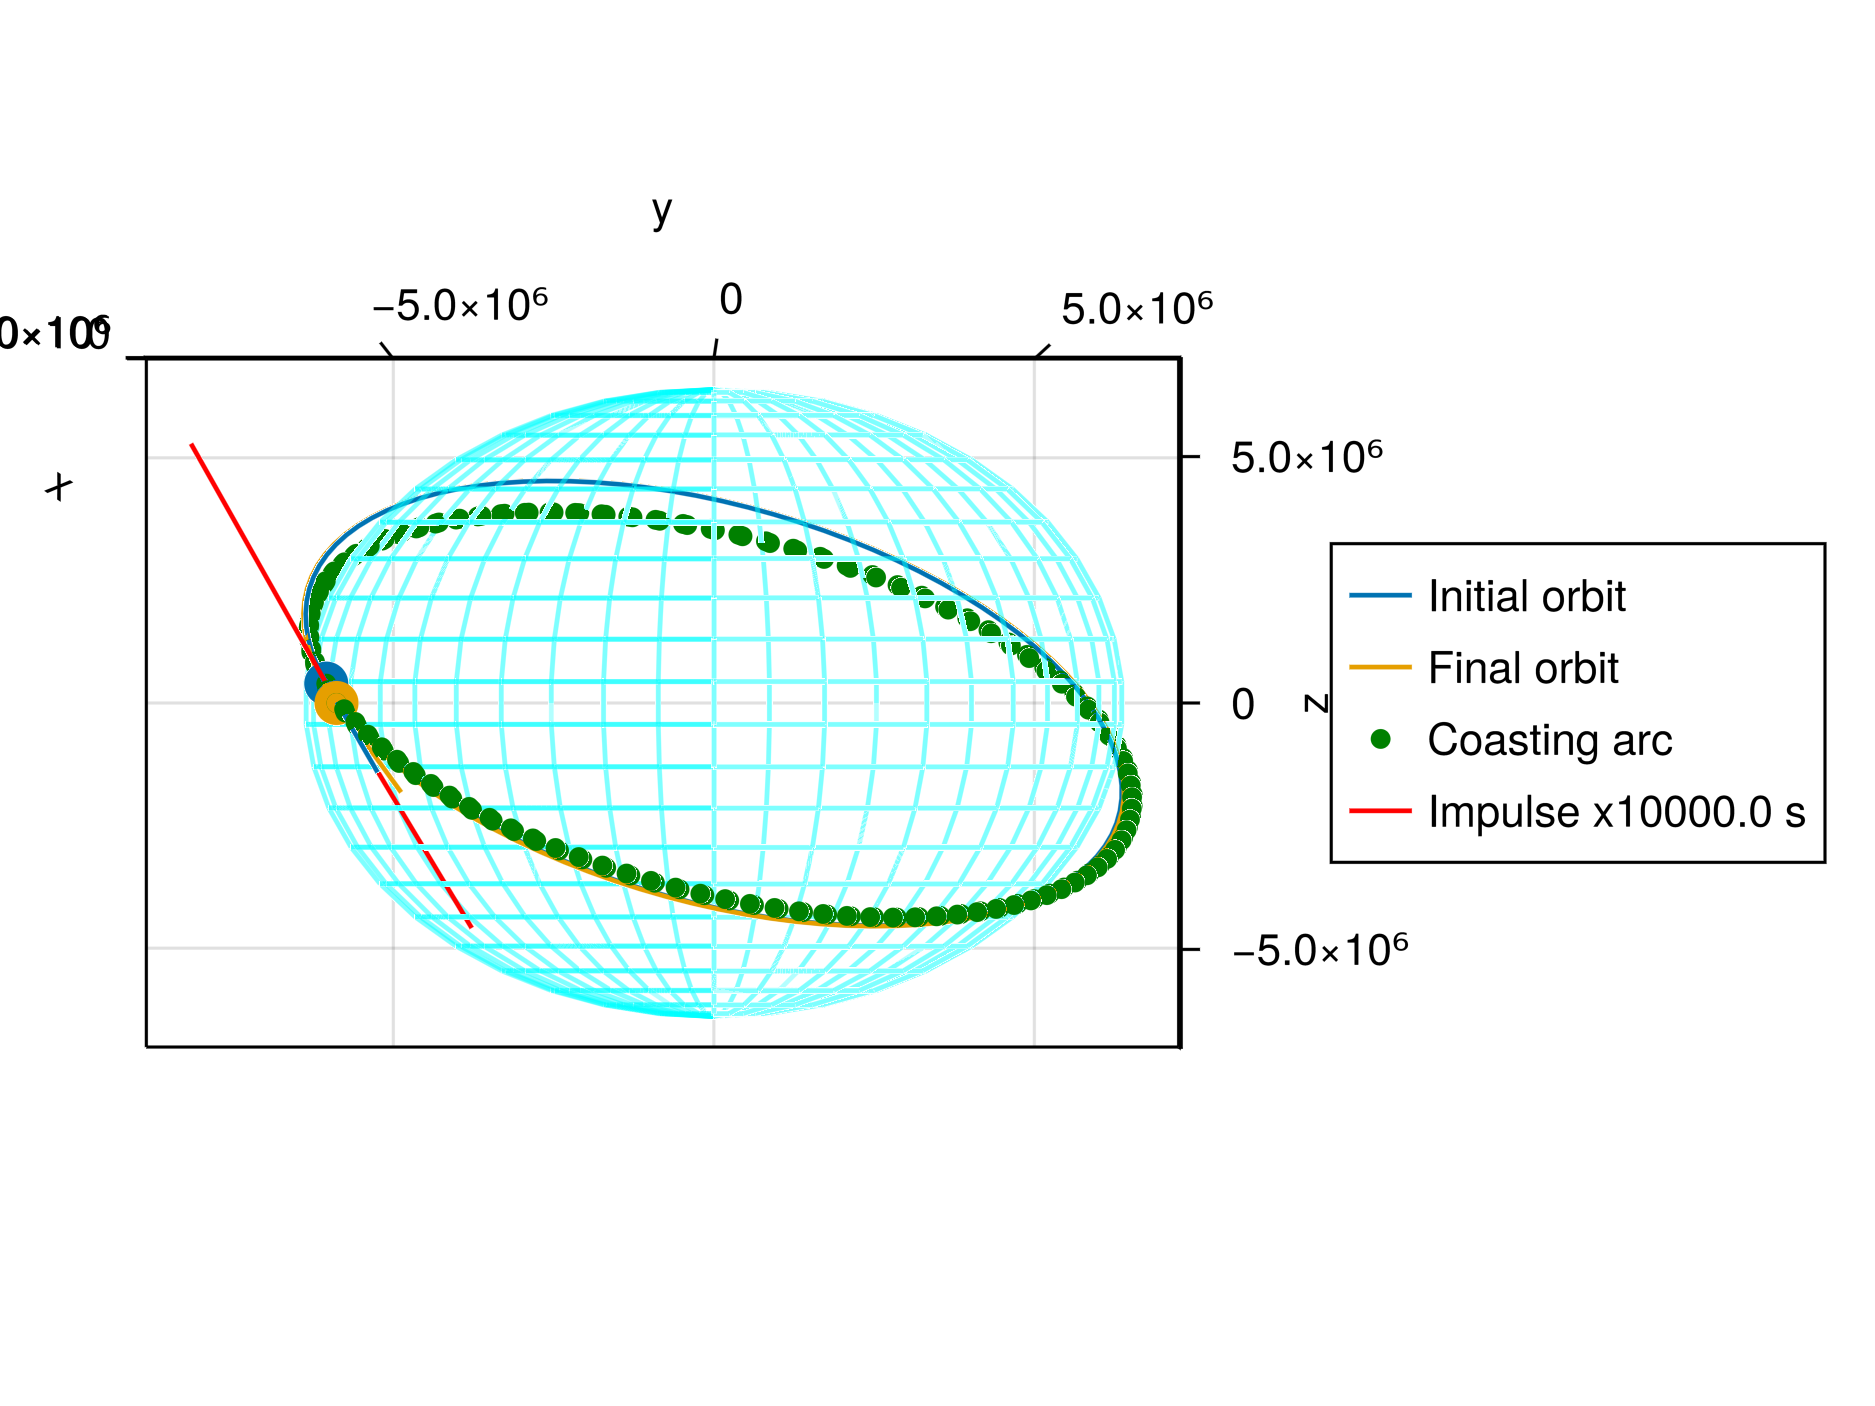
\includegraphics[width=\linewidth]{../results/j2/ipv_noncop/ICI_x+.png}
        \caption{View from x+ axis.}
    \end{subfigure}
    \begin{subfigure}{0.49\linewidth}
        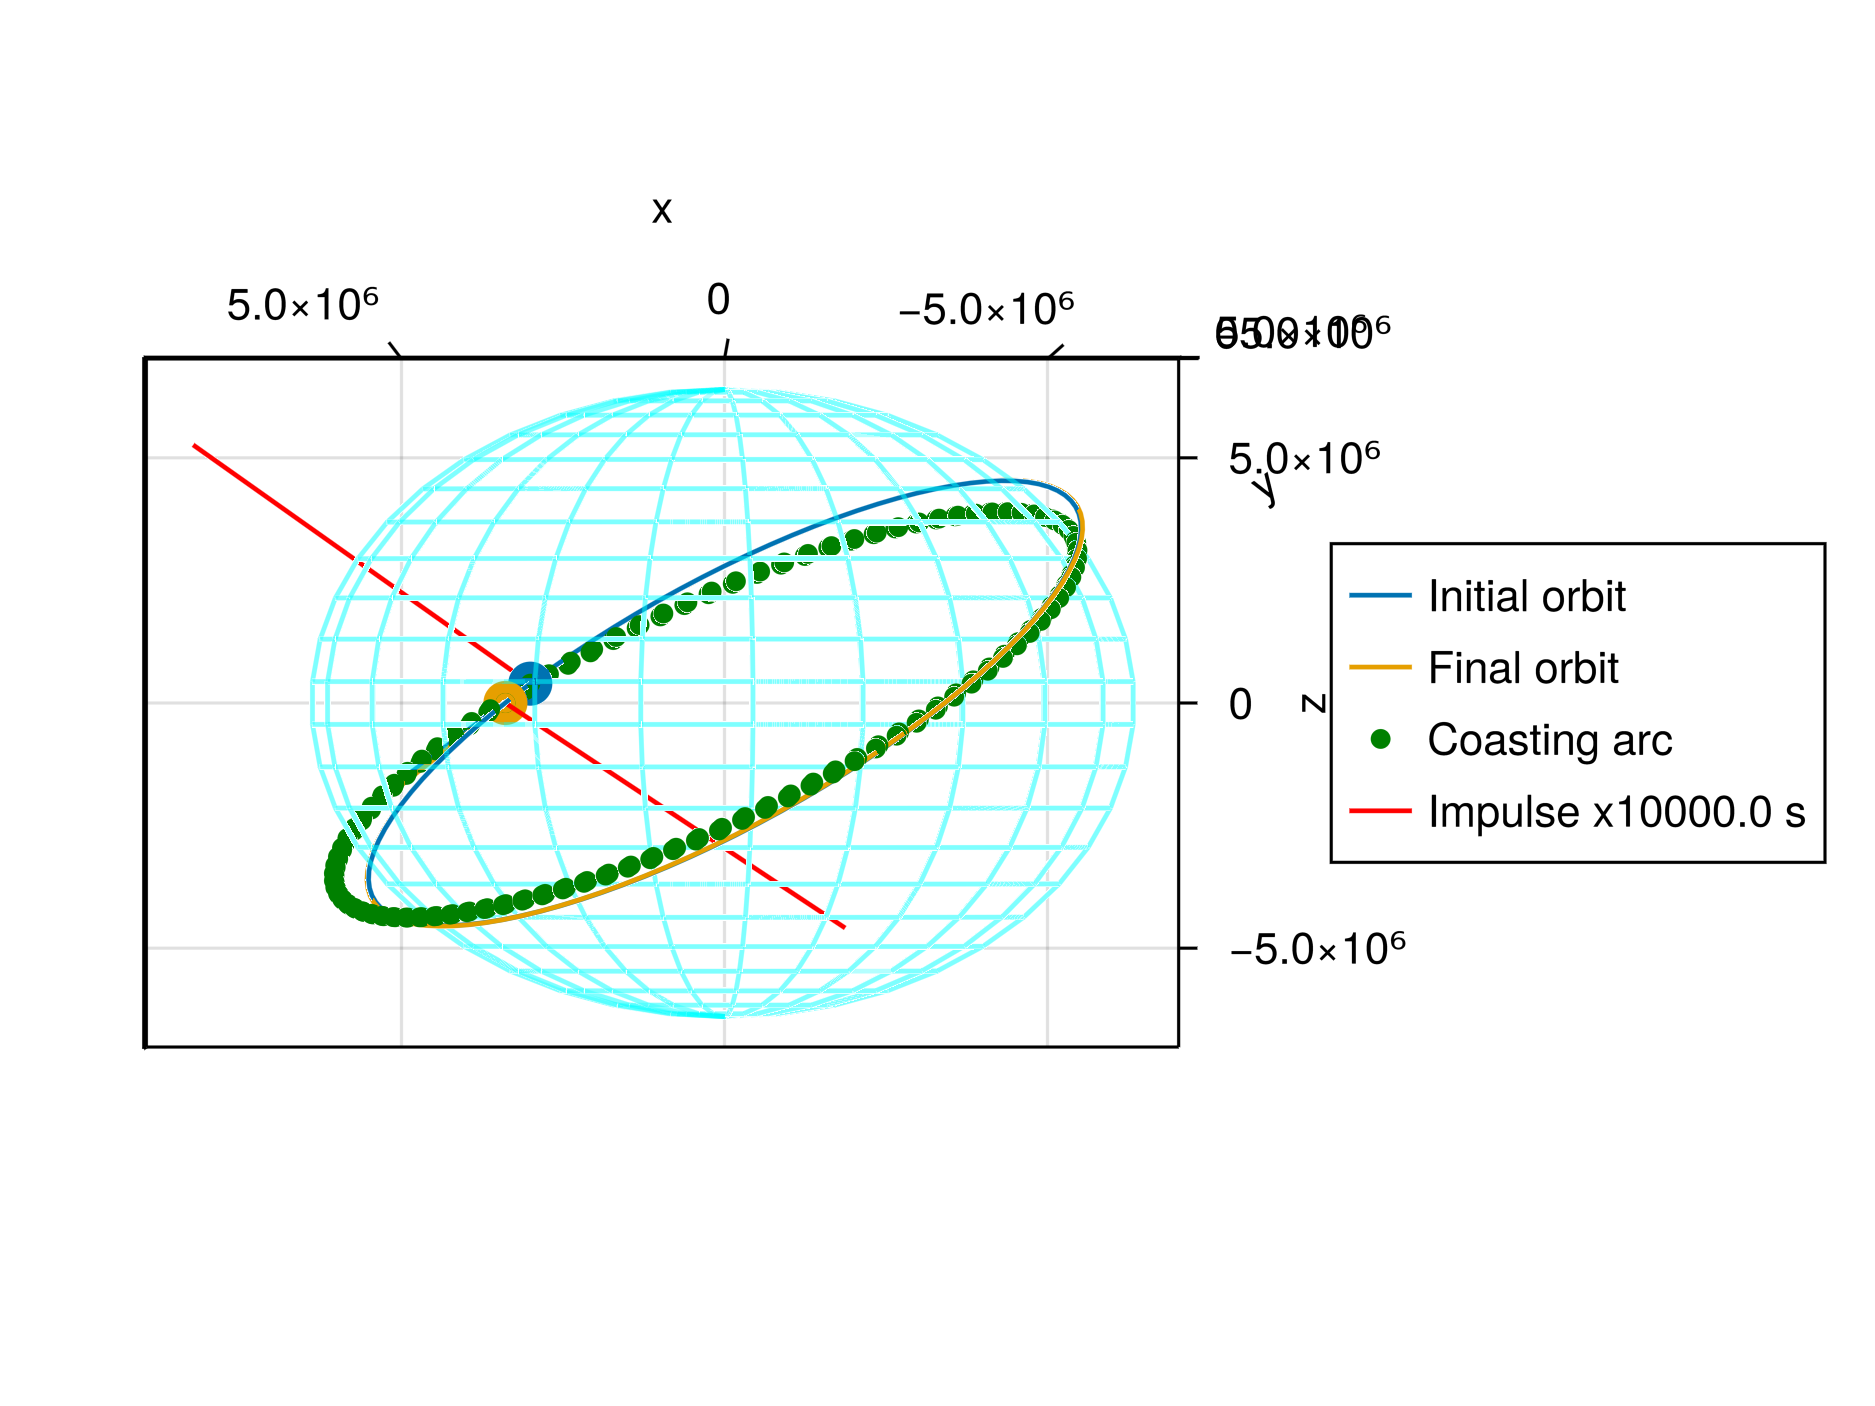
\includegraphics[width=\linewidth]{../results/j2/ipv_noncop/ICI_y+.png}
        \caption{View from y+ axis.}
    \end{subfigure}
    \begin{subfigure}{0.49\linewidth}
        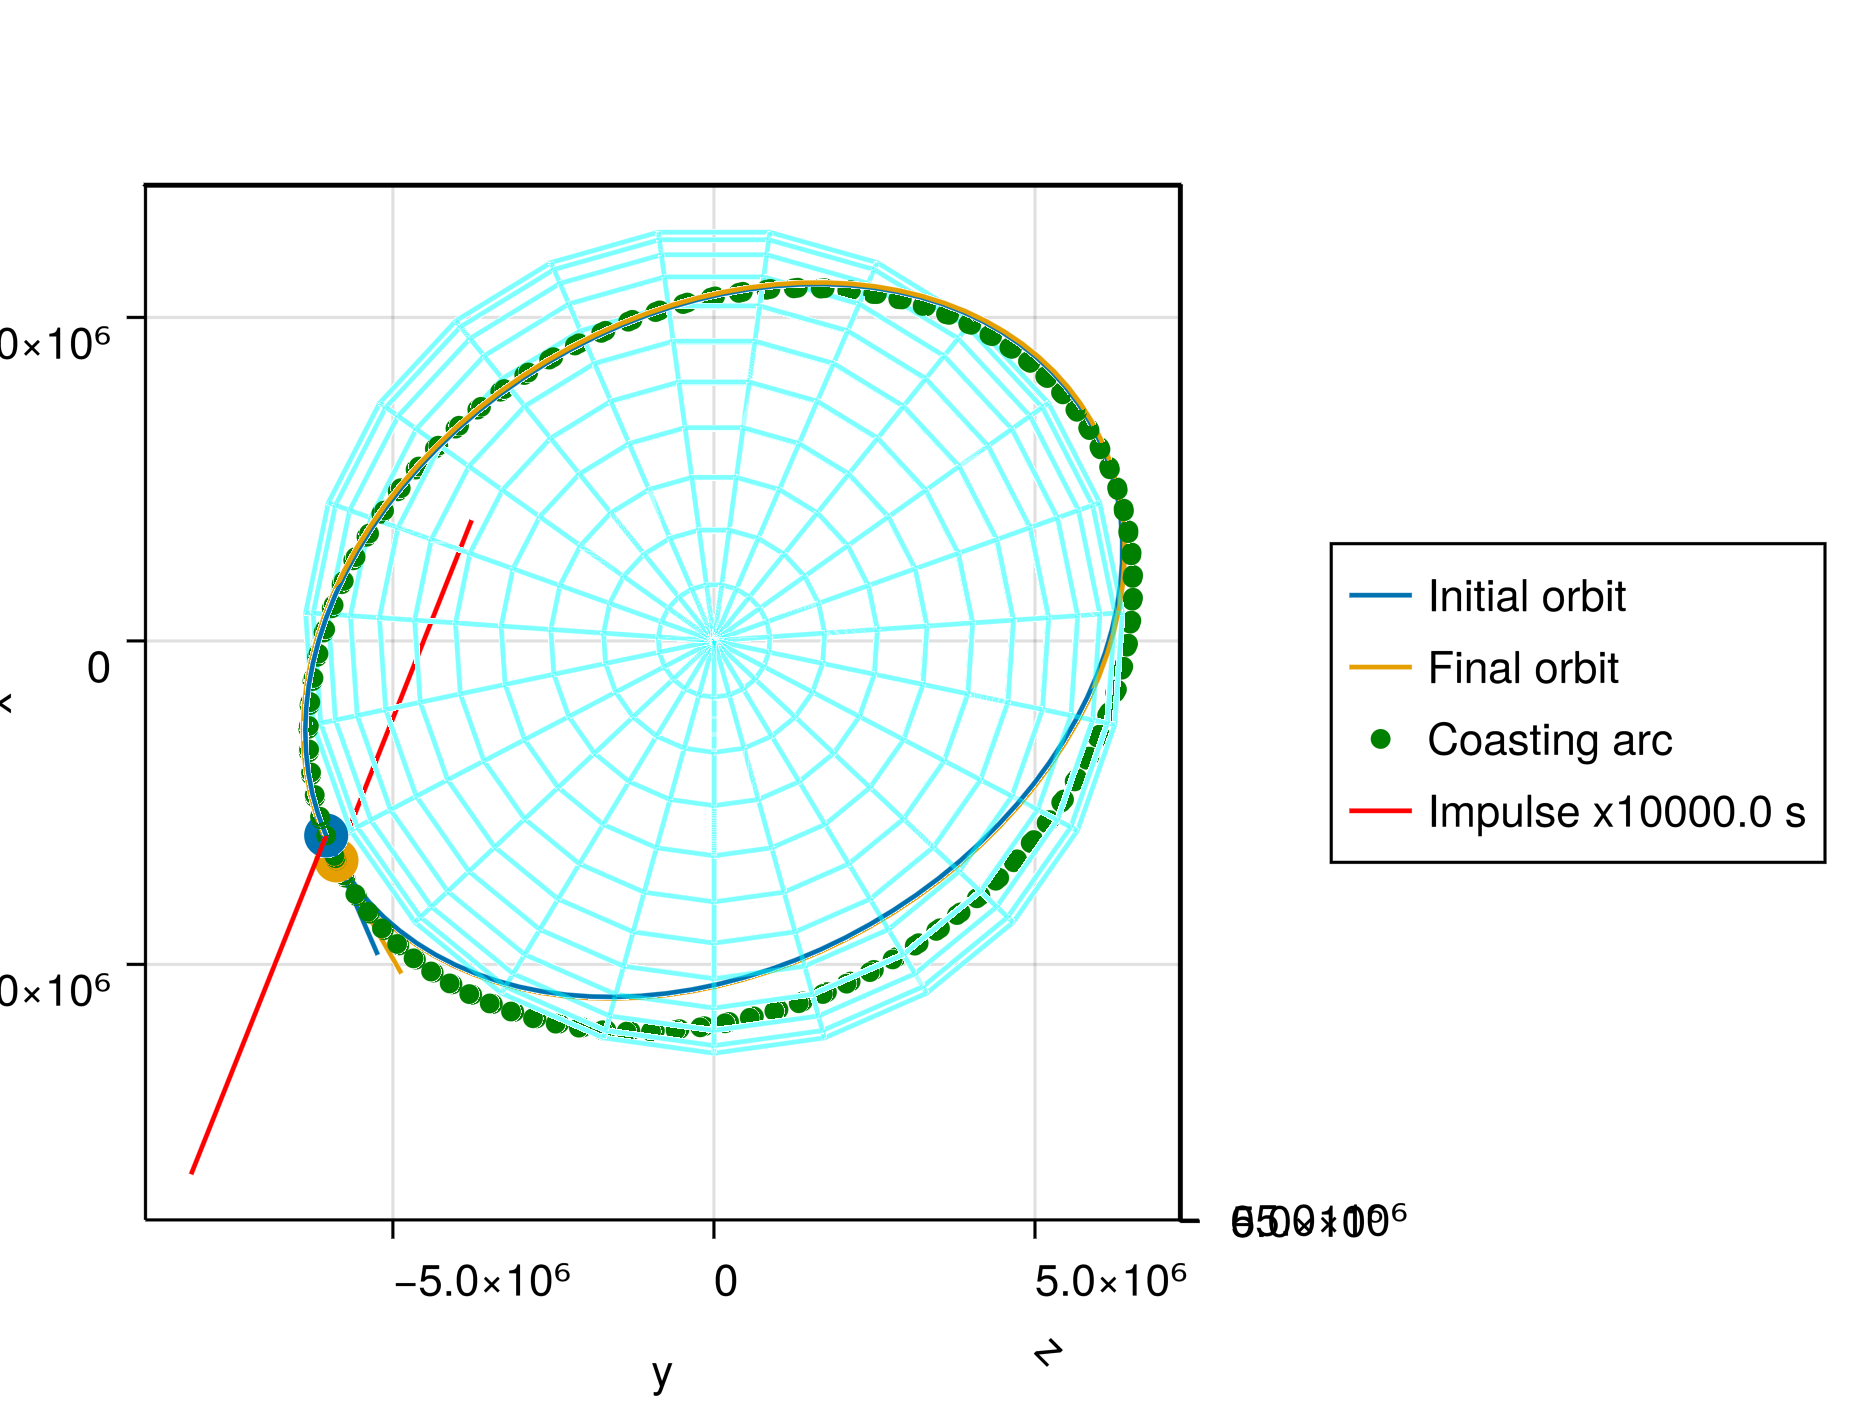
\includegraphics[width=\linewidth]{../results/j2/ipv_noncop/ICI_z+.png}
        \caption{View from z+ axis.}
    \end{subfigure}
    \caption{Circle to circle \texttt{ICI} maneuver 3D view and projections}
    \label{fig:j2_ncop_ICI_figs}
\end{figure}

\begin{figure}[htbp]
    \centering
    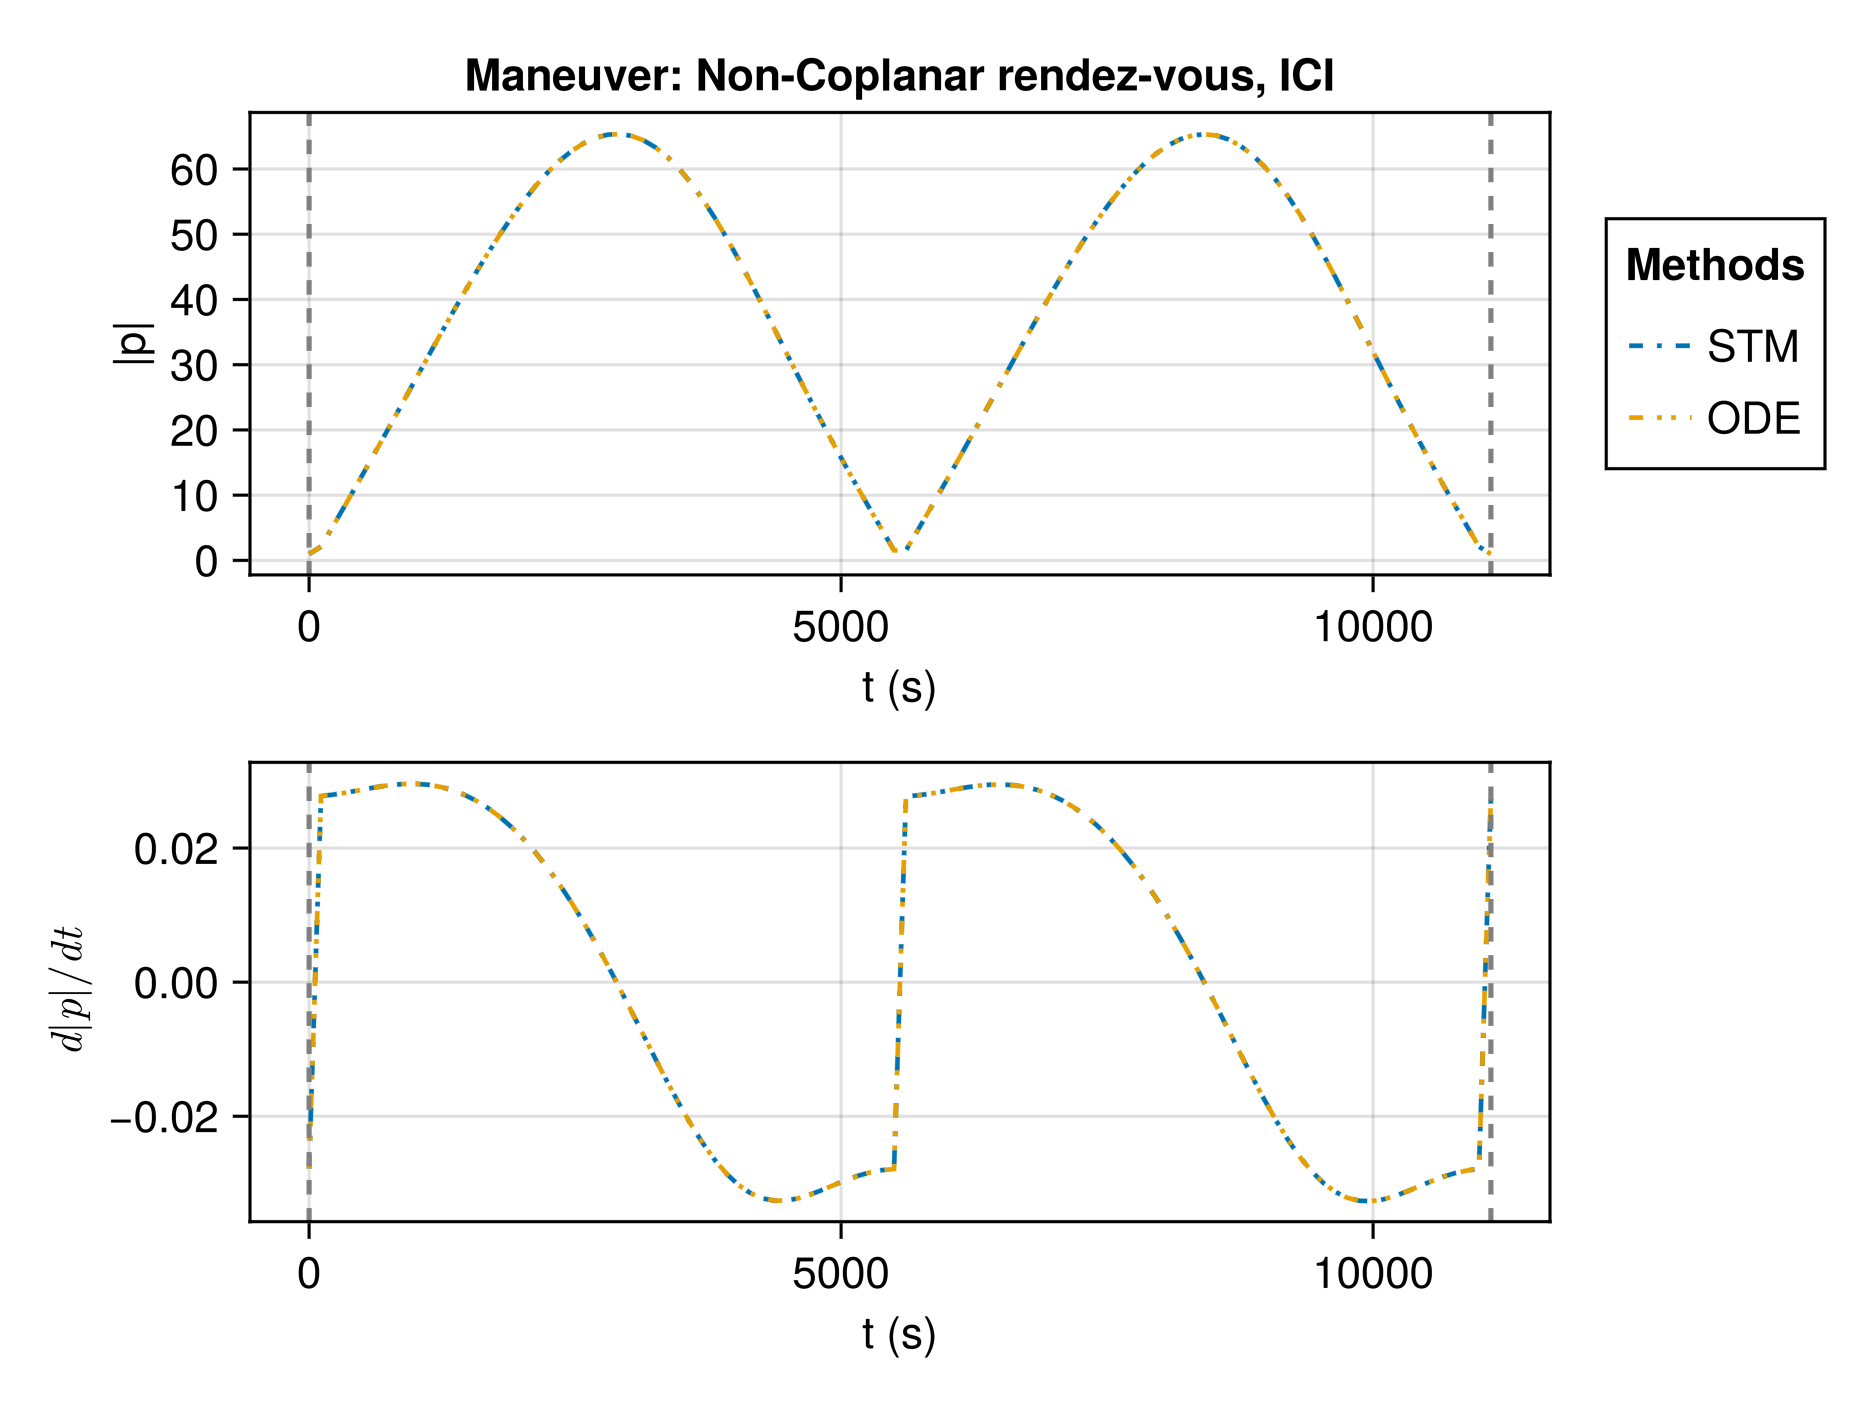
\includegraphics[width=\linewidth]{../results/j2/ipv_noncop/ICI_primer_vector.png}
    \caption{Primer vector trajectory for J2 circle to circle \texttt{ICI} rendez-vous.}
    \label{fig:j2_ncop_ICI_pv}
\end{figure}

The \texttt{CICIC} maneuver is summarized in Table~\ref{tab:j2_ncop_CICIC_tab}, its primer vector trajectory is shown in Figure~\ref{fig:j2_ncop_CICIC_pv}, and its spatial views are shown in Figure~\ref{fig:j2_ncop_CICIC_figs}. Now, this maneuver is only \(5 m/s\) more expensive than its two body counterpart (compare with Table~\ref{tab:tb_ncop_CICIC_tab}), but the impulse magnitudes and times are considerably different. The spatial trajectory does not deviate far from the initial and final orbits, sign of low \(\Delta v\) usage. The primer vector trajectory is now continuous, but still violates the necessary conditions. Now, adding an impulse is necessary.

\begin{table}[htpb]
    \centering
    \begin{tabular}{cccc} \toprule
    \multicolumn{2}{c}{\textbf{Maneuver type}} & \multicolumn{2}{c}{CICIC} \\ \midrule
    \(L\) (m) & \(T\) (s) & \(\varepsilon\) & \(\Delta x_{f}\) (m)    \\ \midrule
    6.7631e6          & 11107.158          & 1.00e-05                & 0.0                        \\ \midrule
    \(\max \lVert p \rVert\) & 3.8353     & \textbf{Diagnostic}   & Add impulse        \\ \midrule
    \textbf{Impulse} & \(t\) (s) & \(\Delta v\) (m/s) & \(1 - p \cdot \hat{u}\) \\ \midrule
    1                 & 7080.30484          & 24.12503             & -0.0                    \\
    2                 & 10011.10872          & 34.14936             & 0.0                    \\\midrule
    \textbf{Total}   & 11107.1576          & 58.27439             &                     \\ \bottomrule   
    \end{tabular}
    \caption{Summary of optimization for J2 noncoplanar \texttt{CICIC} rendez-vous.}
    \label{tab:j2_ncop_CICIC_tab}
\end{table}

\begin{figure}[htbp]
    \centering
    \begin{subfigure}{0.49\linewidth}
        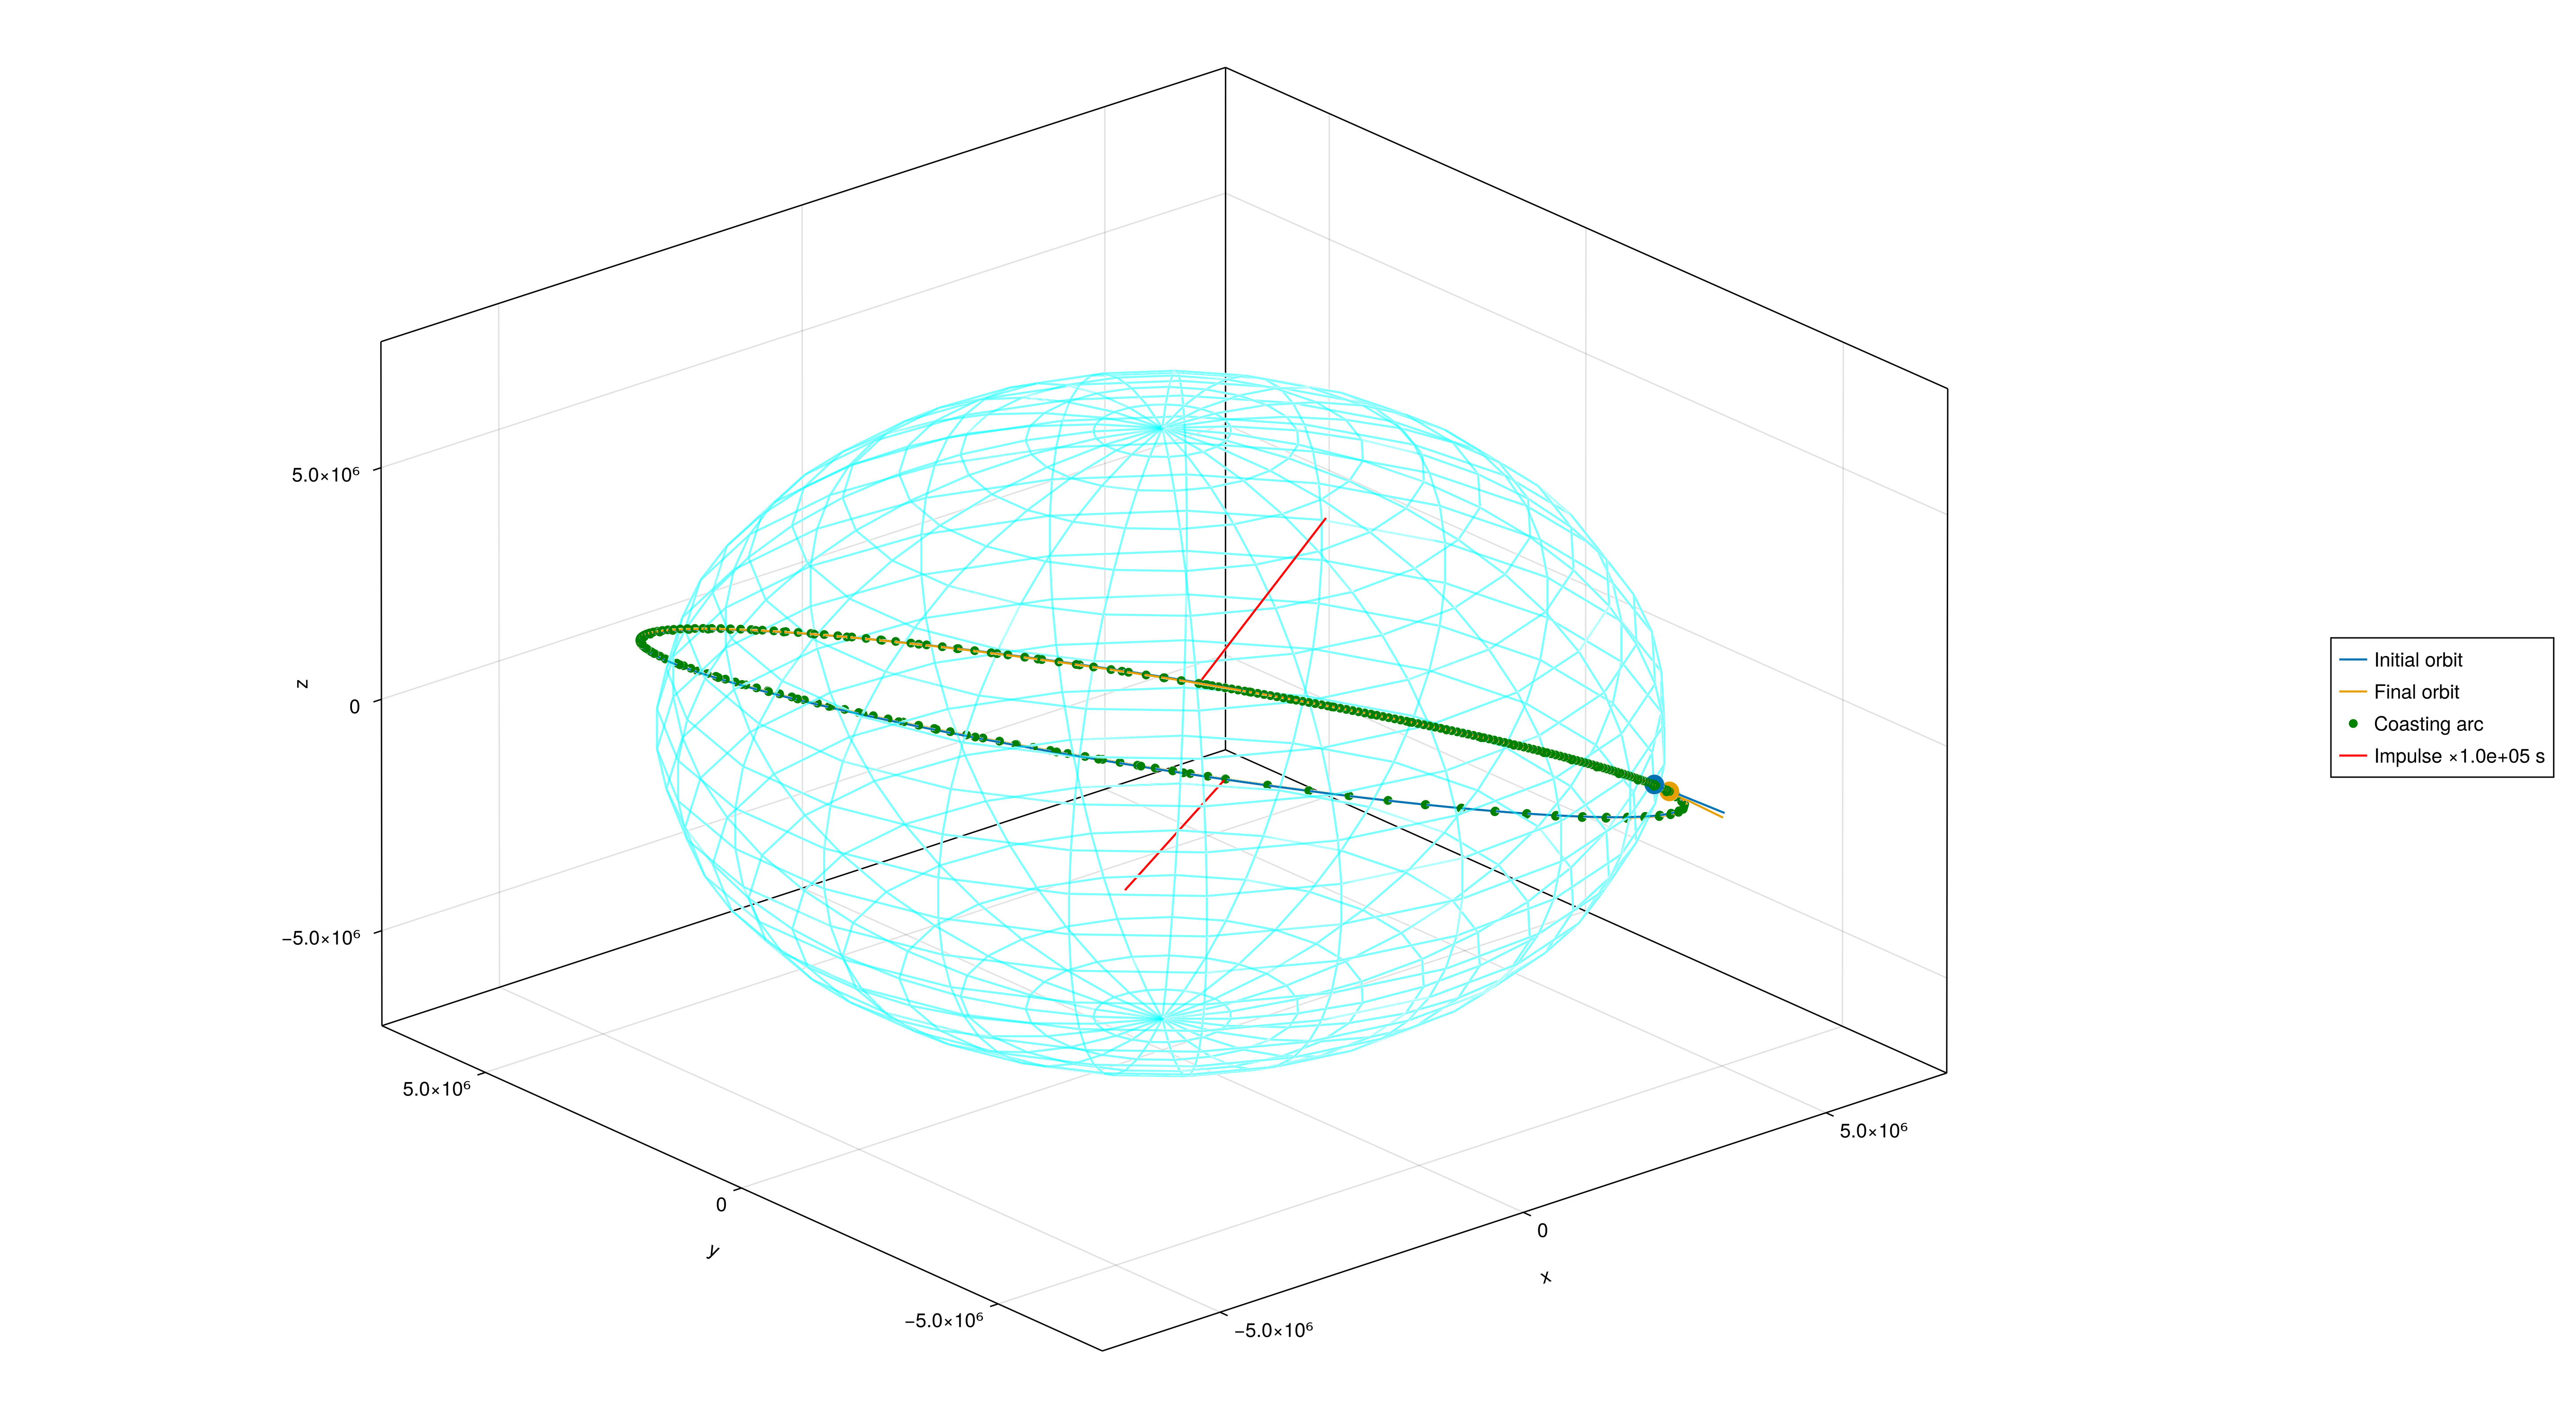
\includegraphics[width=\linewidth]{../results/j2/ipv_noncop/CICIC_3d.png}
        \caption{3D view.}
    \end{subfigure}
    \begin{subfigure}{0.49\linewidth}
        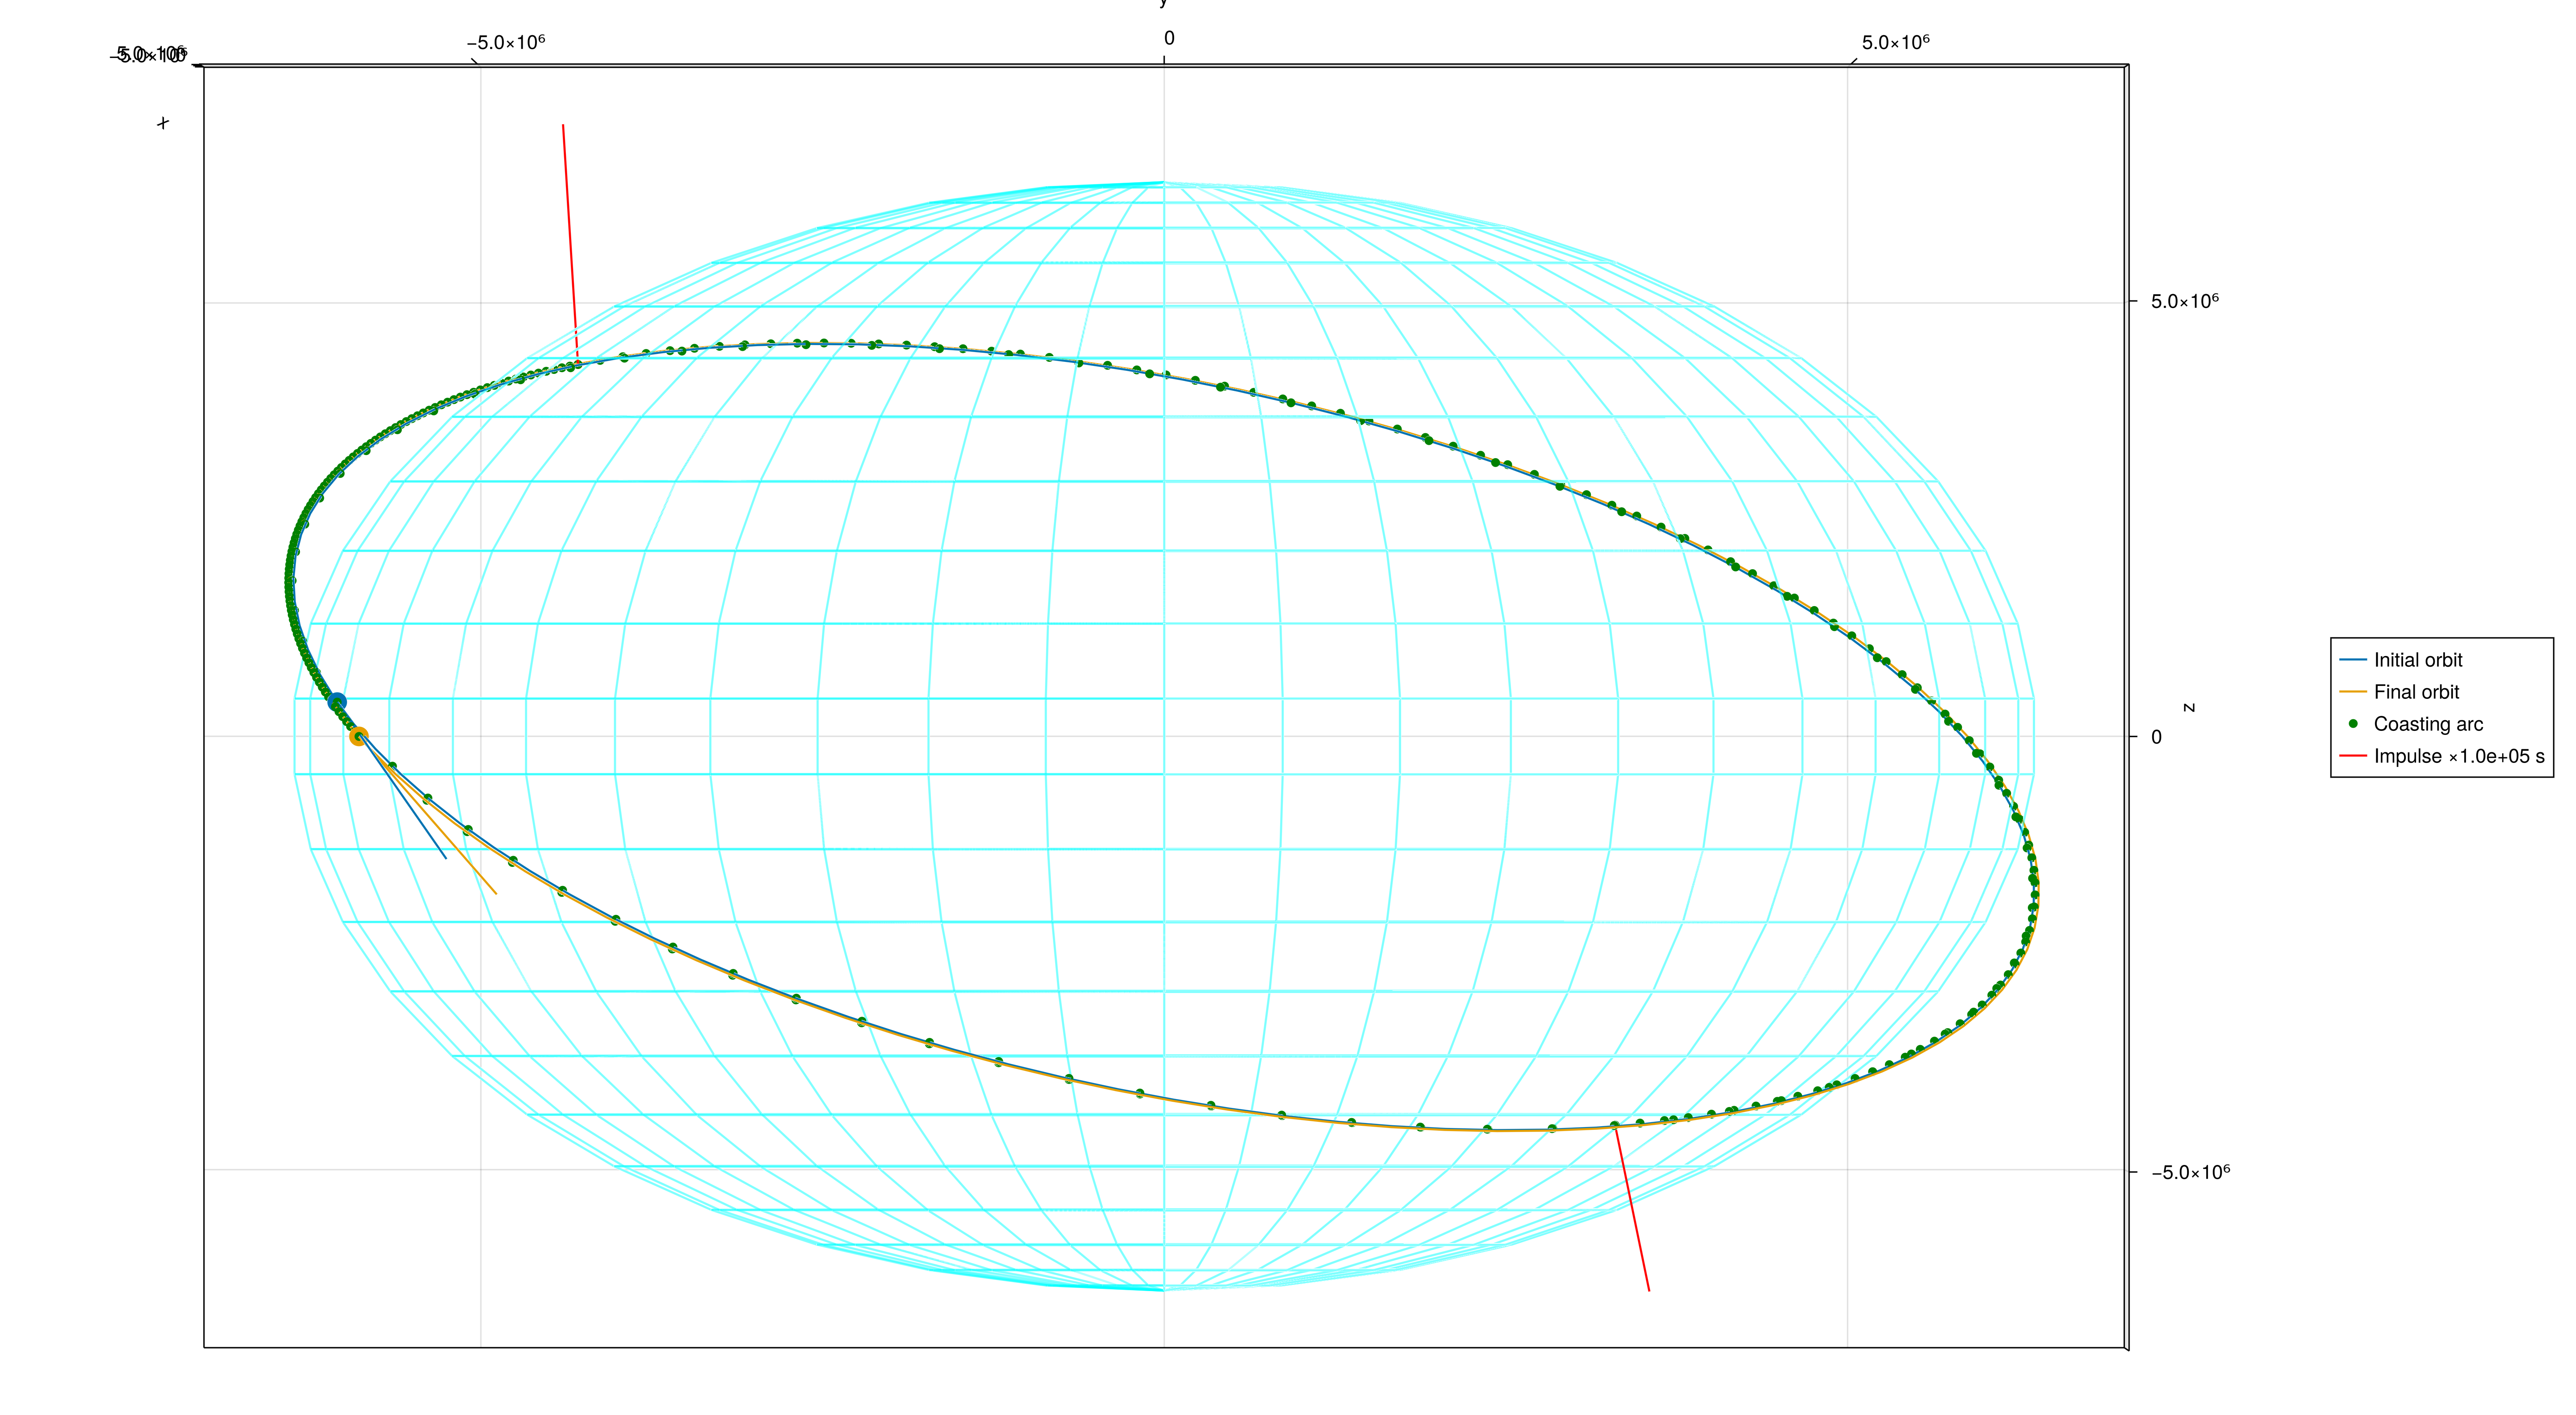
\includegraphics[width=\linewidth]{../results/j2/ipv_noncop/CICIC_x+.png}
        \caption{View from x+ axis.}
    \end{subfigure}
    \begin{subfigure}{0.49\linewidth}
        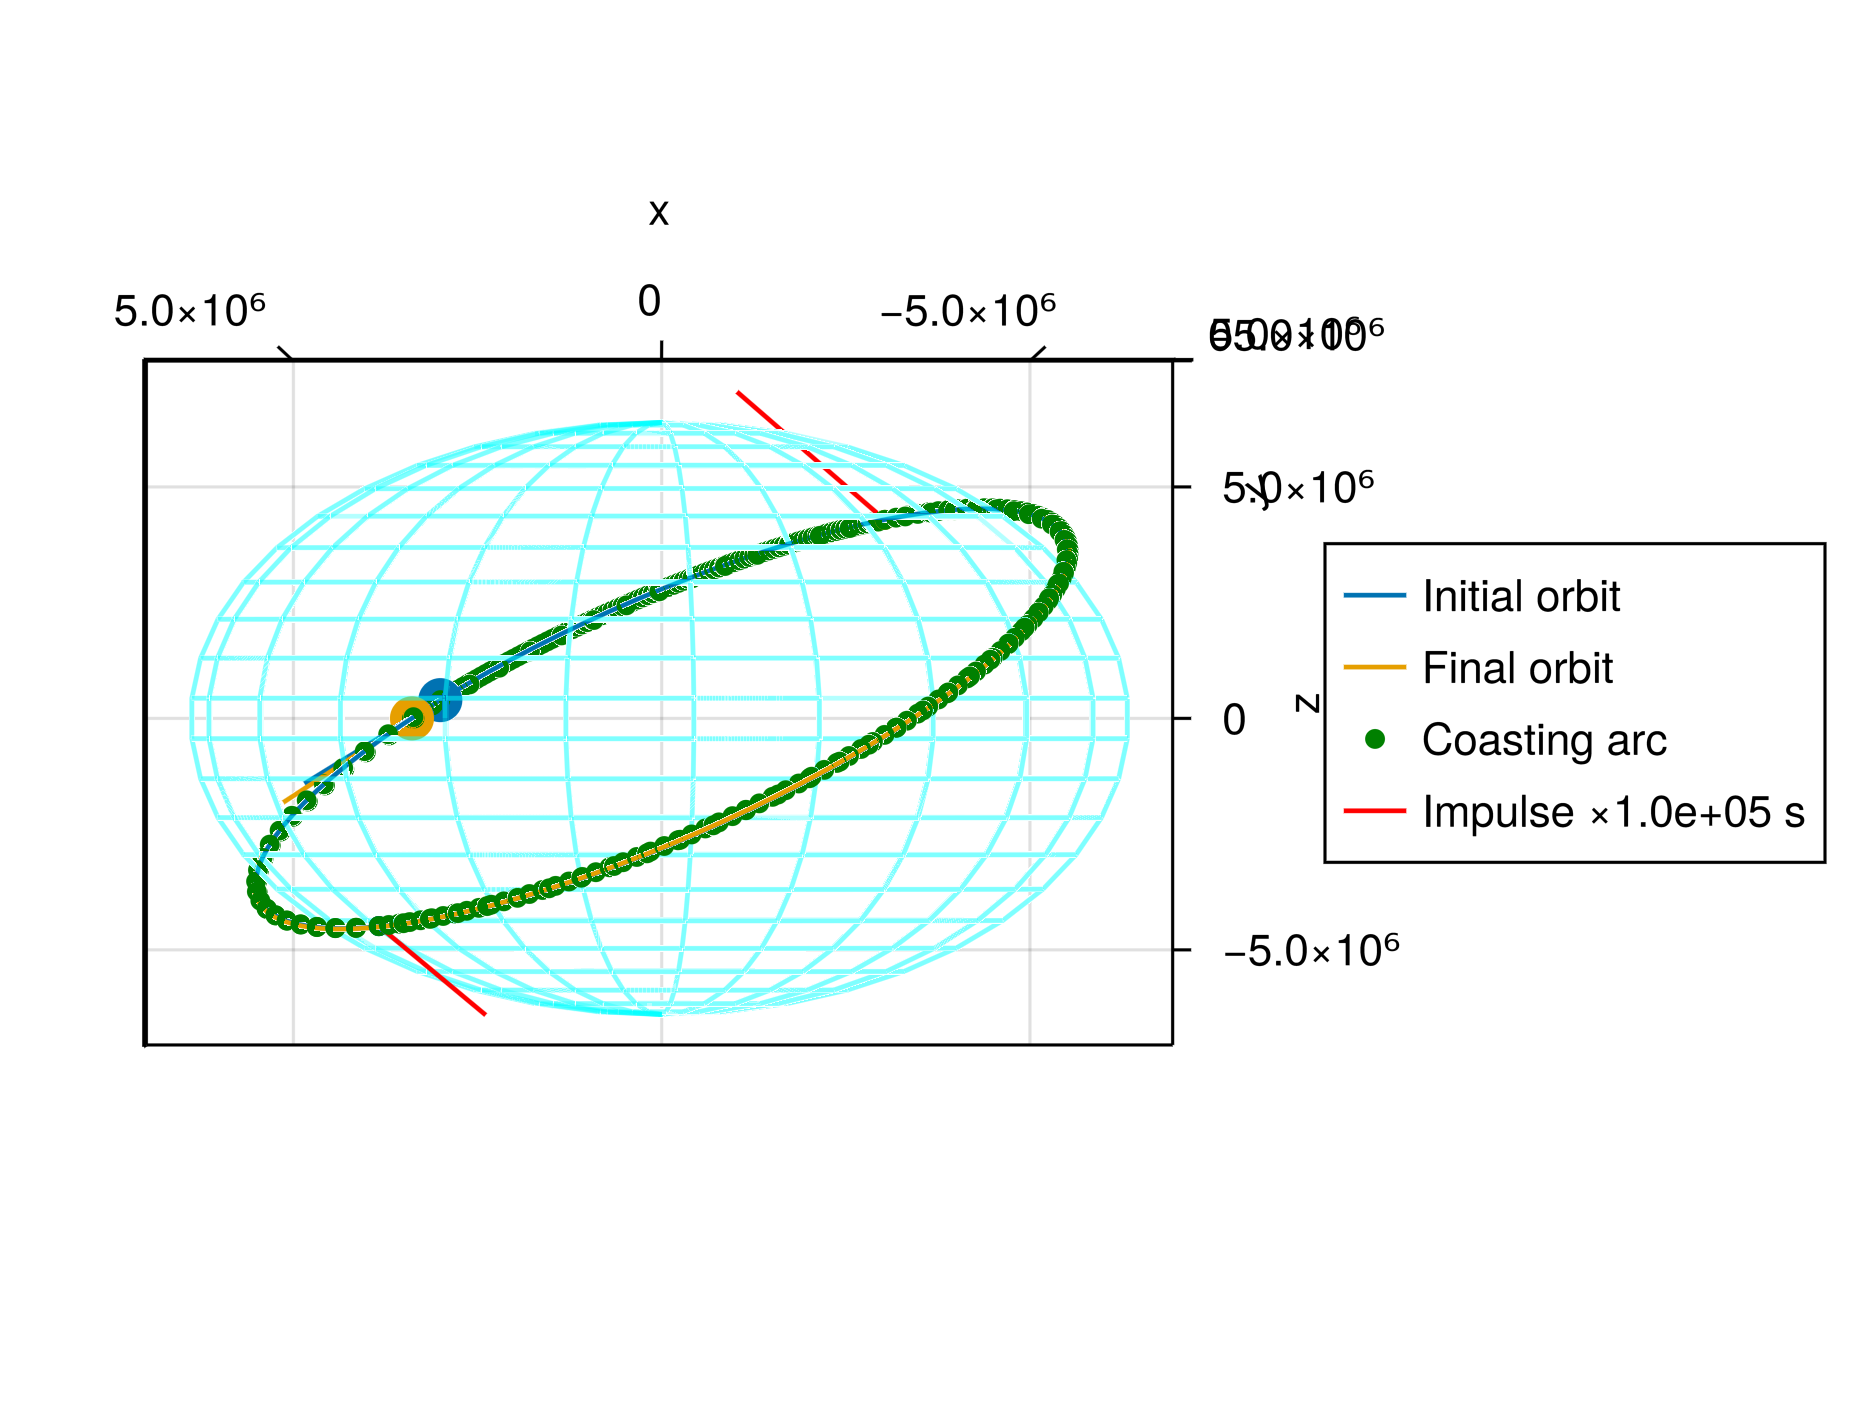
\includegraphics[width=\linewidth]{../results/j2/ipv_noncop/CICIC_y+.png}
        \caption{View from y+ axis.}
    \end{subfigure}
    \begin{subfigure}{0.49\linewidth}
        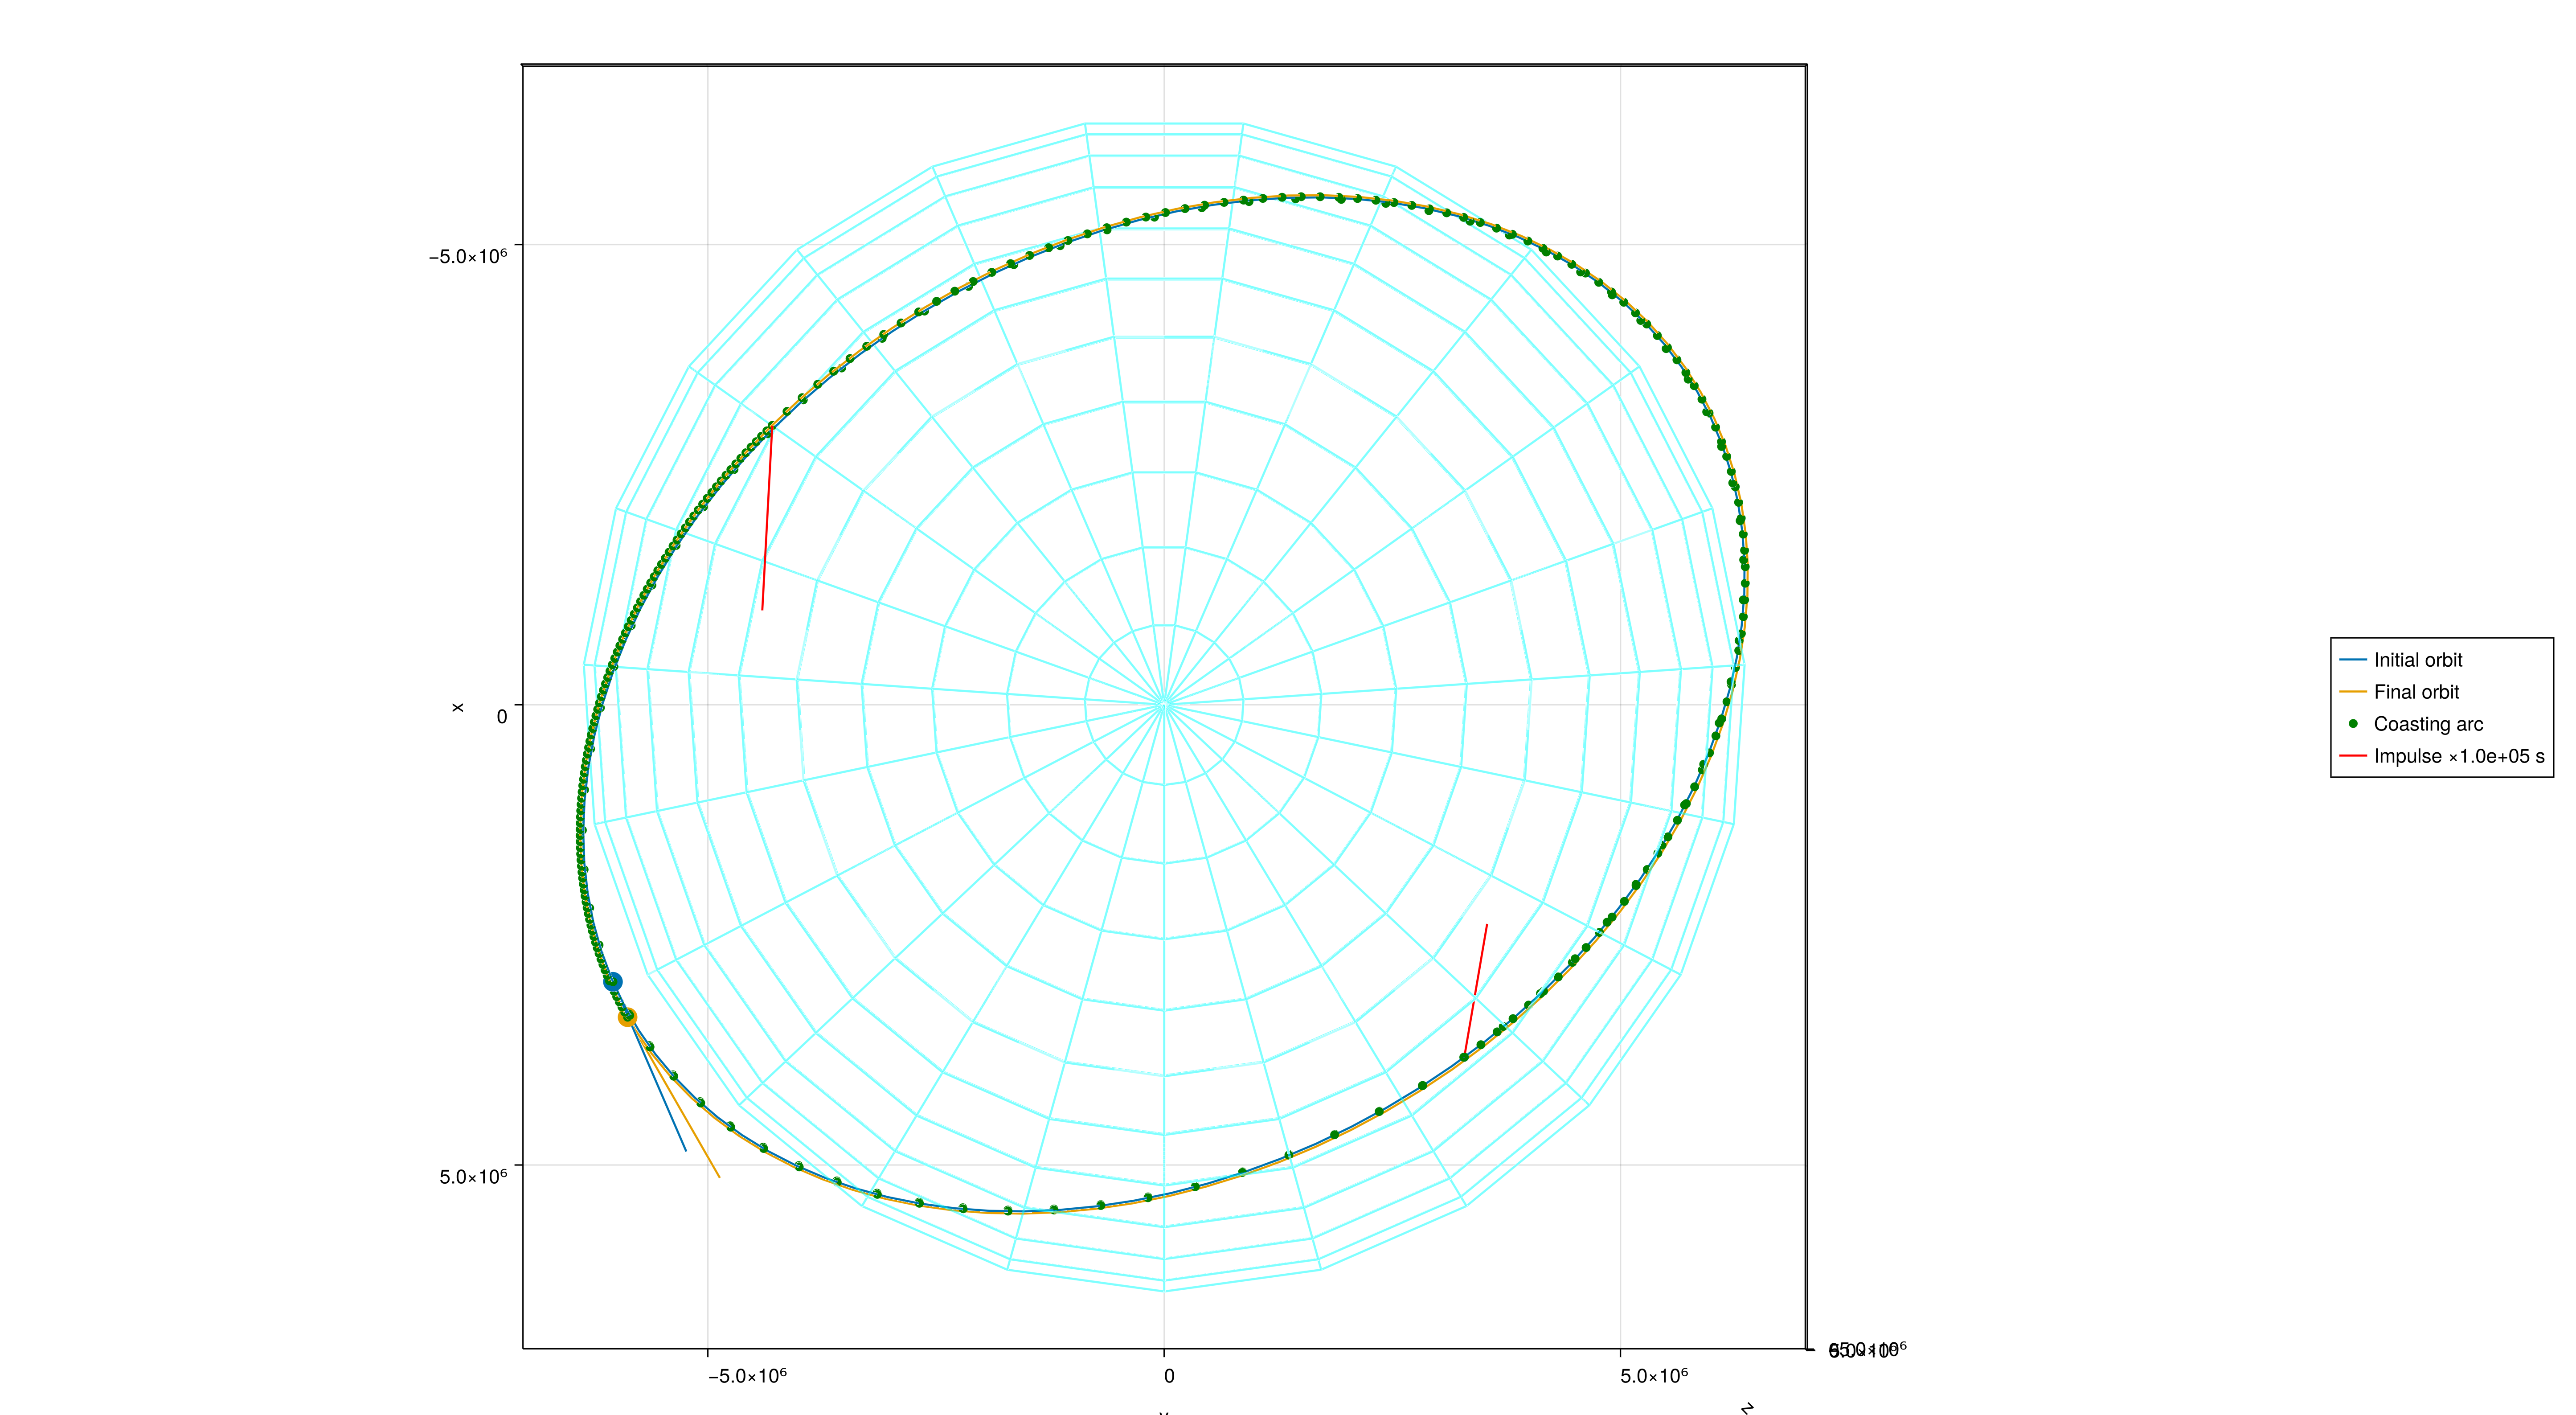
\includegraphics[width=\linewidth]{../results/j2/ipv_noncop/CICIC_z+.png}
        \caption{View from z+ axis.}
    \end{subfigure}
    \caption{Circle to circle \texttt{CICIC} maneuver 3D view and projections}
    \label{fig:j2_ncop_CICIC_figs}
\end{figure}

\begin{figure}[htbp]
    \centering
    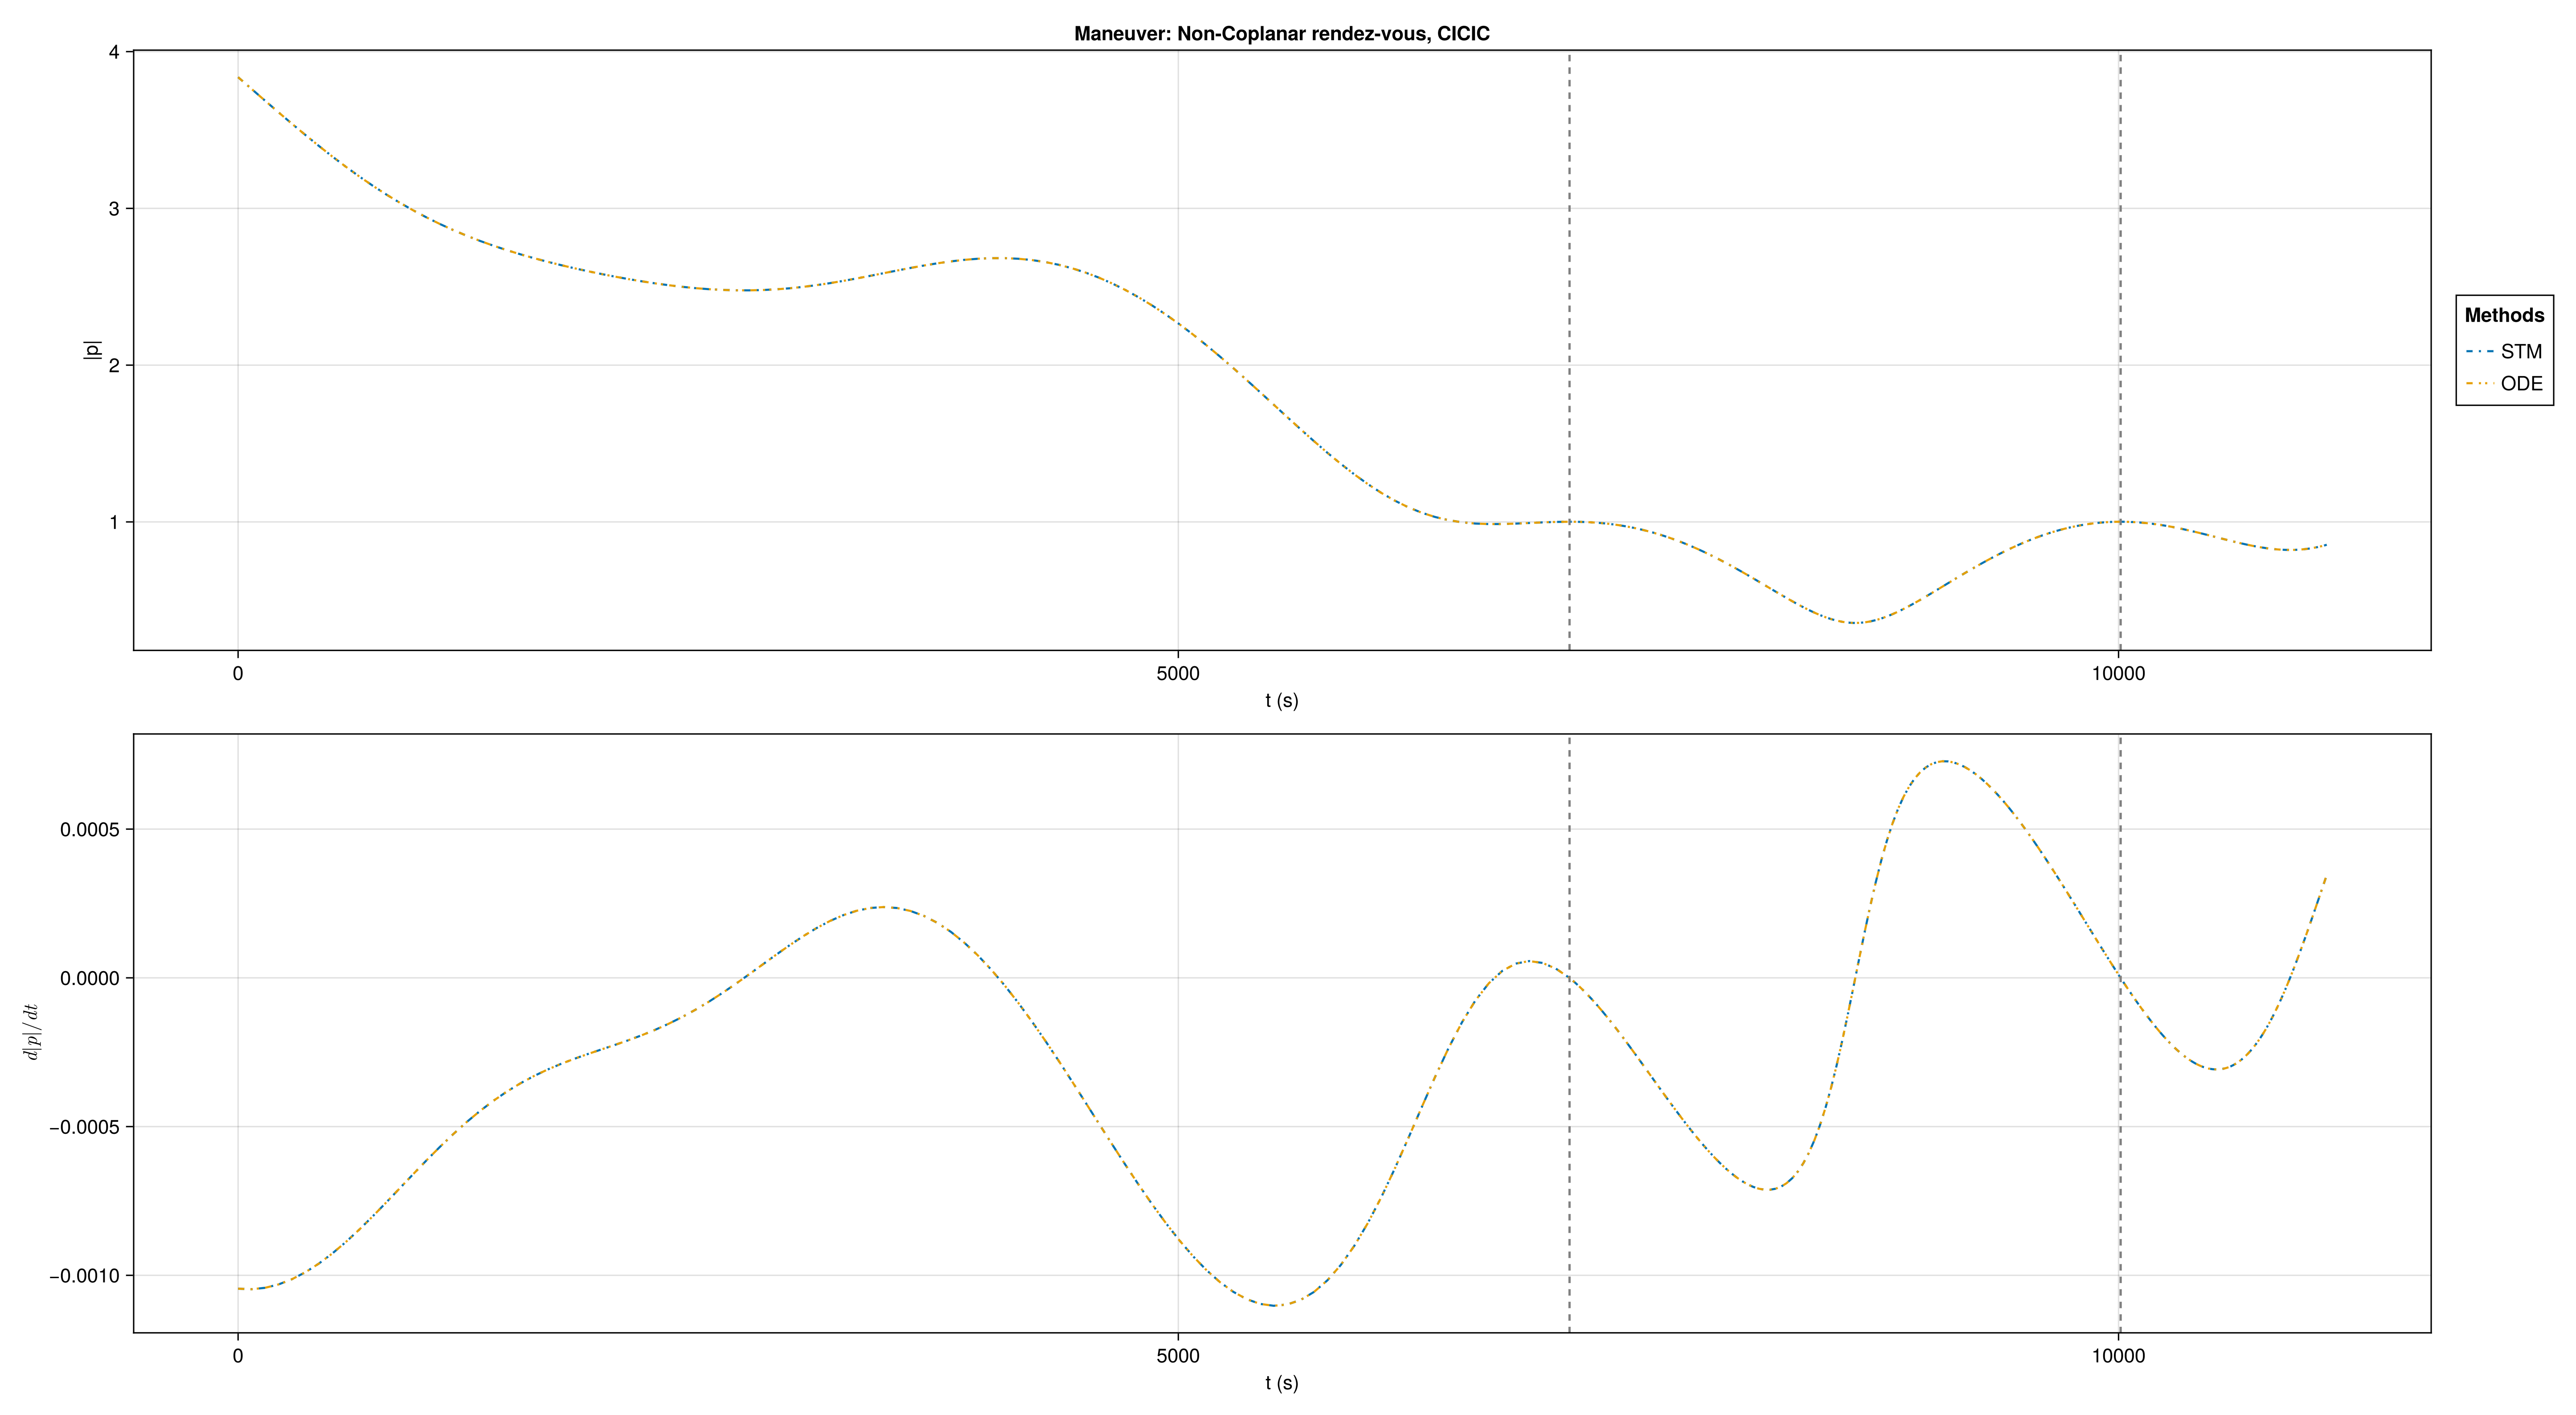
\includegraphics[width=\linewidth]{../results/j2/ipv_noncop/CICIC_primer_vector.png}
    \caption{Primer vector trajectory for J2 circle to circle \texttt{CICIC} rendez-vous.}
    \label{fig:j2_ncop_CICIC_pv}
\end{figure}

A \texttt{CICICIC} maneuver was solved next, with summary in Table~\ref{tab:j2_ncop_CICICIC_tab}, primer vector trajectory in Figure~\ref{fig:j2_ncop_CICICIC_pv} and the spatial views are omitted due to the trajectory being visually indistinct to initial and final orbits. The cost is marginally lower than the previous case, but now the primer vector necessary conditions are satisfied. It is worth clarifying that they require that \(\lVert \mathbf{p} \rVert = 1\) at every impulse time, but this does not mean that unity norm cannot occur outside impulse times, which exactly what happens at around \(4000 s\) in this case. 

\begin{table}[htpb]
    \centering
    \begin{tabular}{cccc} \toprule
    \multicolumn{2}{c}{\textbf{Maneuver type}} & \multicolumn{2}{c}{CICICIC} \\ \midrule
    \(L\) (m) & \(T\) (s) & \(\varepsilon\) & \(\Delta x_{f}\) (m)    \\ \midrule
    6.7631e6          & 11107.158          & 1.00e-05                & 0.0                        \\ \midrule
    \(\max \lVert p \rVert\) & 1.0     & \textbf{Diagnostic}   & Local Optimum        \\ \midrule
    \textbf{Impulse} & \(t\) (s) & \(\Delta v\) (m/s) & \(1 - p \cdot \hat{u}\) \\ \midrule
    1                 & 1676.61473          & 5.84342             & -0.0                    \\
    2                 & 7185.69293          & 20.83452             & -0.0                    \\
    3                 & 9942.01138          & 29.32859             & -0.0                    \\\midrule
    \textbf{Total}   & 11107.1576          & 56.00653             &                     \\ \bottomrule   
    \end{tabular}
    \caption{Summary of optimization for J2 noncoplanar \texttt{CICICIC} rendez-vous.}
    \label{tab:j2_ncop_CICICIC_tab}
\end{table}

\begin{figure}[htbp]
    \centering
    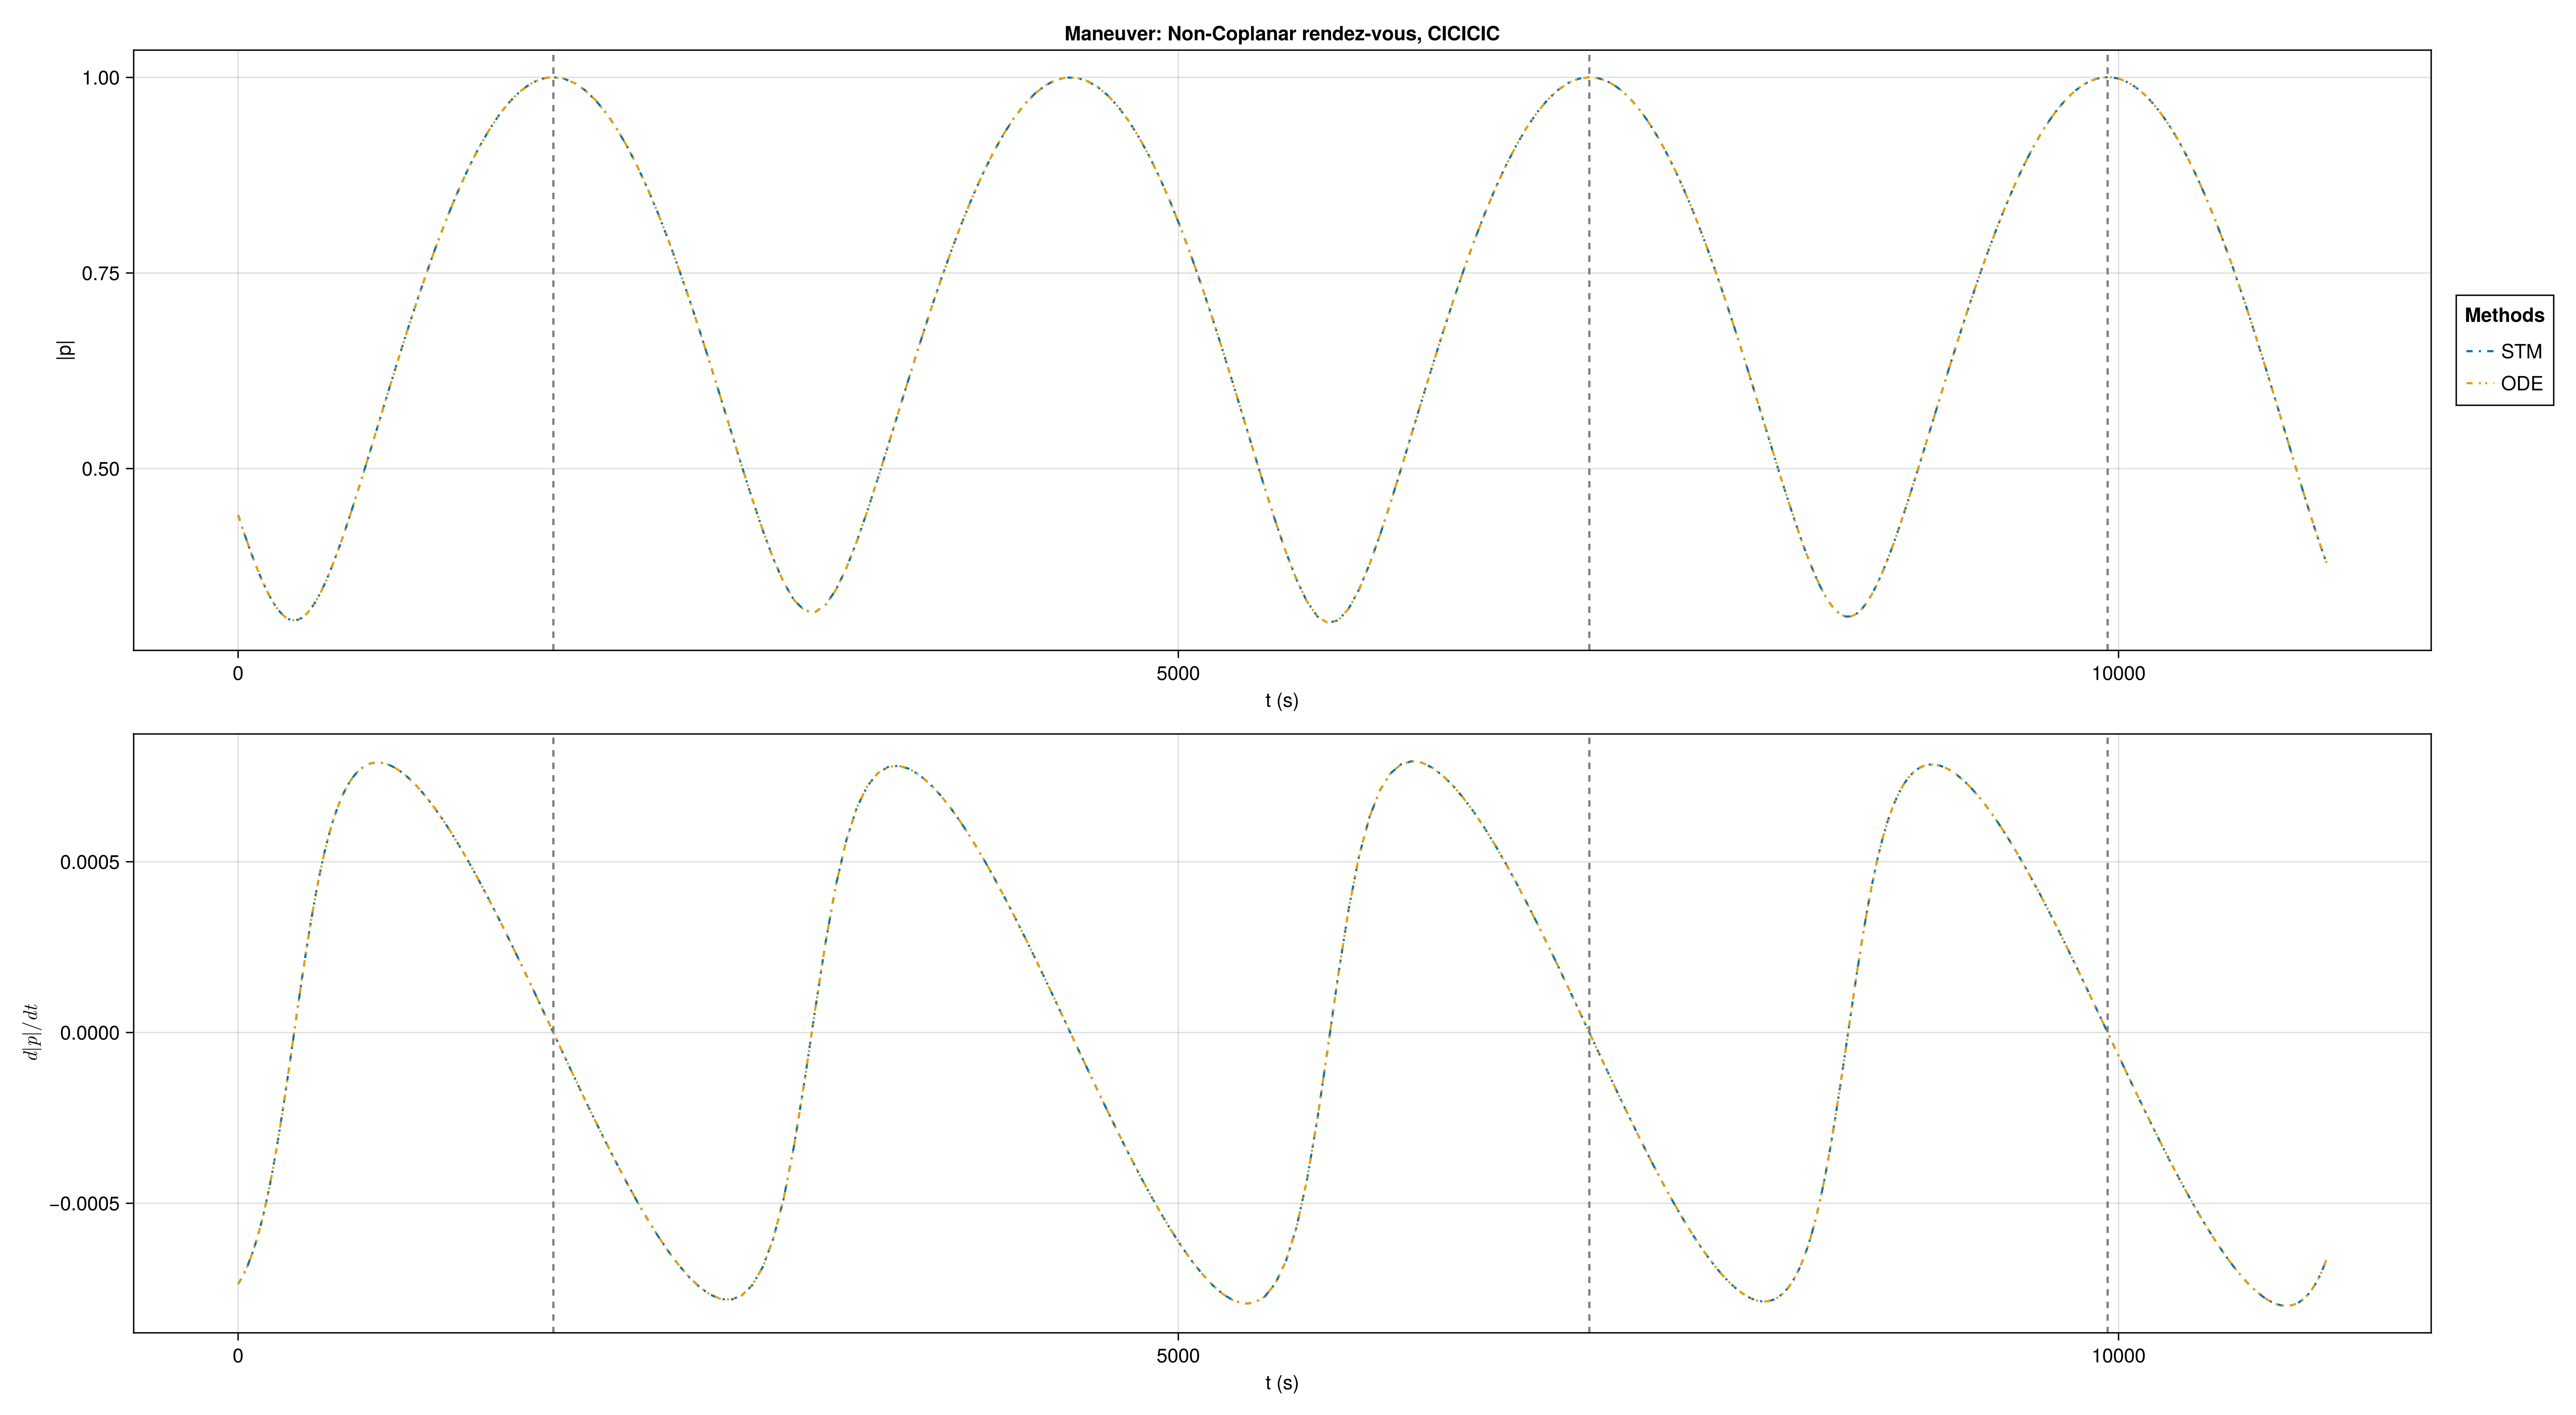
\includegraphics[width=\linewidth]{../results/j2/ipv_noncop/CICICIC_primer_vector.png}
    \caption{Primer vector trajectory for J2 circle to circle \texttt{CICICIC} rendez-vous.}
    \label{fig:j2_ncop_CICICIC_pv}
\end{figure}


\newpage
\FloatBarrier
\section{J2 and Drag}

Finally, the non-conservative model of J2 and drag disturbances is tackled. This model's results will be presented in a summarized fashion, since they were found to be almost identical to J2 results. In addition, although the theory predicts that only the ODE method of primer vector calculation should work for this system, it was found that the STM method gave almost identical trajectories. Both of those findings will be discussed based on the \texttt{ICI} maneuver of the circle-to-circle scenario.

\subsection{Circle to Circle}

The circle to circle case was solved in a \texttt{ICI} maneuver case, summarized in Table~\ref{tab:jd_c2c_ICI_tab}. Straightaway, it is clear that these results are numerically identical to the ones found in the J2 model, given in Table~\ref{tab:j2_c2c_ICI_tab}. This can be easily explained by the fact that the effects of drag are some orders of magnitude weaker than J2 effects and, above all, they do not change the trajectories categorically like J2 does. That is, J2 makes trajectories noncoplanar, but drag does not introduce any particular behavior that is noticeable in short time spans like this.
    
\begin{table}[htpb]
    \centering
    \begin{tabular}{cccc} \toprule
    \multicolumn{2}{c}{\textbf{Maneuver type}} & \multicolumn{2}{c}{ICI} \\ \midrule
    \(L\) (m) & \(T\) (s) & \(\varepsilon\) & \(\Delta x_{f}\) (m)    \\ \midrule
    8.0e6          & 1.0          & 1.00e-05                & 0.49712                        \\ \midrule
    \(\max \lVert p \rVert\) & 563.46     & \textbf{Diagnostic}   & Initial + Final coast        \\ \midrule
    \textbf{Impulse} & \(t\) (s) & \(\Delta v\) (m/s) & \(1 - p \cdot \hat{u}\) \\ \midrule
    1                 & 0.0          & 5209.4779             & -0.0                    \\
    2                 & 3560.54079          & 4318.71793             & -0.0                    \\\midrule
    \textbf{Total}   & 3560.54079          & 9528.19583             &                     \\ \bottomrule   
    \end{tabular}
    \caption{Summary of optimization for J2+Drag circle-to-circle \texttt{ICI} rendez-vous.}
    \label{tab:jd_c2c_ICI_tab}
\end{table}

The primer vector trajectory in Figure~\ref{fig:jd_c2c_ICI_pv} compares the STM and ODE methods for this maneuver. As a reminder, the theory from Section~\ref{sssec:pv_calc_ncon} disallows, in general, the use of the STM method with non-conservative models. However, as can be seen, both methods give almost identical primer vector trajectories.

\begin{figure}[htbp]
    \centering
    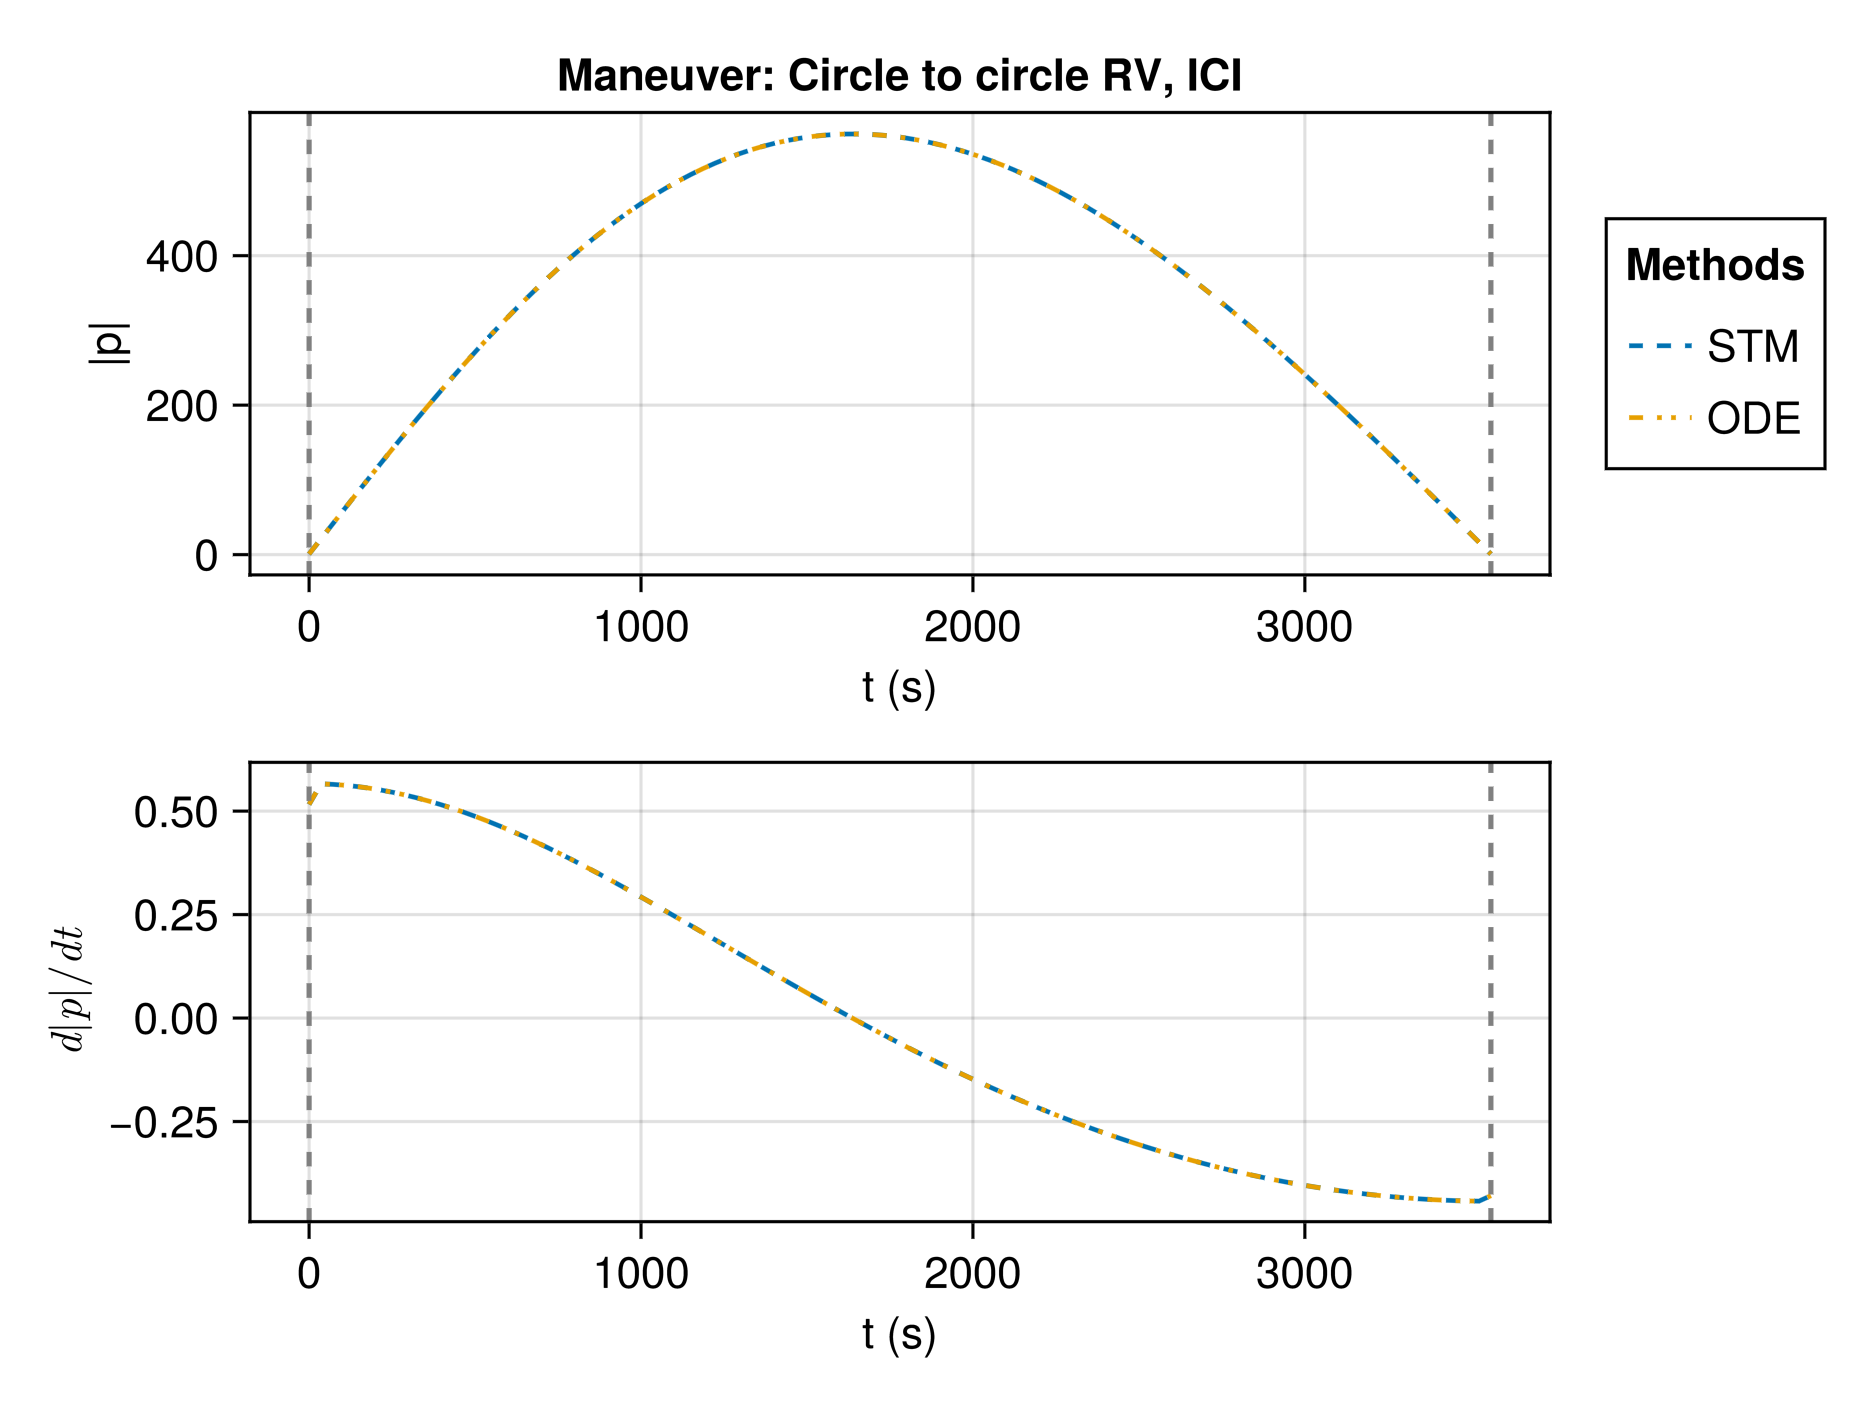
\includegraphics[width=\textwidth]{../results/j2drag/hohmann/ICI_primer_vector.png}
    \caption{Primer vector trajectory for J2+Drag circle to circle \texttt{ICI} rendez-vous.}
    \label{fig:jd_c2c_ICI_pv}
\end{figure}

This can be explained by comparing the matrices \(A_\delta\) and \(A_p\), the coefficients of the ODEs of the STM and ODE transition matrices respectively. They are only expected to differ in the lower right quadrant:
\begin{align}
    (A_\delta)_{4\leq i \leq 6, 4 \leq j \leq 6} &= \begin{bmatrix}
        -5.56731-12 & 0.0 & 0.0 \\
        0.0 & -7.77221e-12    & -2.72282e-12 \\
        0.0 & -2.72282e-12    & -8.92972e-12 \\
    \end{bmatrix} \\
    (A_p)_{4\leq i \leq 6, 4 \leq j \leq 6} &= \begin{bmatrix}
        5.56731e-12 & 0.0 & 0.0 \\
        0.0 & 7.77221e-12 & 2.72282e-12 \\
        0.0 & 2.72282e-12 & 8.92972e-12 \\
    \end{bmatrix}
\end{align}

Indeed, the matrices satisfy \(A_\delta = - A_p^T\), as predicted, but due to the low intensity of drag forces, they are both close to \(\mathbf{0}_{3\times 3}\), which is the lower right quadrant of \(A_{p, J2}\), the primer vector ODE coefficient matrix in the J2 model. This shows that maneuvers where drag is weak, either by virtue of the short timespan or high altitude, the effects of drag may be neglected. An open question is whether or not there exists a realistic maneuver scenario where drag effects cause sufficient differences w.r.t.\ to the J2 case.